\documentclass[conference]{IEEEtran}
\IEEEoverridecommandlockouts

\usepackage{cite}
\usepackage{amsmath,amssymb,amsfonts}
\numberwithin{figure}{subsection}
\usepackage{graphicx}
\usepackage{textcomp}
\usepackage{xcolor}
\usepackage[utf8]{inputenc}
\usepackage[labelfont=bf]{caption}
\captionsetup[table]{labelsep=space, 
         justification=raggedright, singlelinecheck=off, labelformat=empty}
\usepackage{kotex}
\usepackage{wrapfig} 
\usepackage{enumitem}
\usepackage{algorithm}
\usepackage{verbatim}
\usepackage{algpseudocode} 
\usepackage{hyperref}
\usepackage{listings}
\usepackage{cleveref, array, booktabs, threeparttable}
\lstset{
   breaklines=true,
   basicstyle=\ttfamily
   }
\def\BibTeX{{\rm B\kern-.05em{\sc i\kern-.025em b}\kern-.08em
    T\kern-.1667em\lower.7ex\hbox{E}\kern-.125emX}}


\title{Smart Wine Cellar – Cave de Vin(Label D)\\ \LARGE DIOnyoS}

\author{\IEEEauthorblockN{Yujin Do}
\IEEEauthorblockA{\textit{College of Engineering}\\ 
\textit{Hanyang University}\\
\textit{Dept. of Information System}\\
Seoul, Korea\\
yujindo9@gmail.com}
\and
\IEEEauthorblockN{Yerin Cho}
\IEEEauthorblockA{\textit{College of Engineering}\\ 
\textit{Hanyang University}\\
\textit{Dept. of Information System}\\
Seoul, Korea\\
forjustice9839@gmail.com}
\and
\IEEEauthorblockN{Jungi Kim}
\IEEEauthorblockA{\textit{College of Engineering}\\ 
\textit{Hanyang University}\\
\textit{Dept. of Information System}\\
Seoul, Korea\\
damnum3@hanyang.ac.kr}
\and
\IEEEauthorblockN{Hyungseo Han}
\IEEEauthorblockA{\textit{College of Engineering}\\ 
\textit{Hanyang University}\\
\textit{Dept. of Information System}\\
Seoul, Korea\\
shorelinesquere@gmail.com}
}


\begin{document}

\maketitle
\thispagestyle{empty}
\pagestyle{empty}
\begin{abstract}
Our team is trying to develop User-Friendly wine cellar by appending additional functions to “LG wine cellar". By capturing and registering wines in "Cave de Vin(label D)", users can effectively manage their wines and wine cellar. Using wine recommendation and purchasing function can promote additional consumptions to wine and wine cellar. Also, by sharing the scene that enjoying wine on the social media, people can enjoy the marketing effect of LG wine cellar.
\end{abstract}

\begin{table}[h!]
\caption{Role Assignments}
\def\arraystretch{1.24} \small
    \begin{tabular}{|p{1.8cm}|p{1.4cm}|p{4.4cm}|}
        \hline
        Roles & Name & Task description and etc. \\ \hline
        Quality\par Assurance Manager&  Hyungseo Han & They understand demand and requirement of application. They test the overall application from customers’ point of view and report error and bug. They strive to maximize user experience by considering UI / UX. \\ \hline
        
        Software \par Developer & Yerin Cho \par Jungi Kim  & Software developers think about the software in general. They design and implement the requirements of application. They also strive to satisfy users and customers. \\ \hline
        
        Development \par manager & Yujin Do & Development manager manages the overall project. They strive to meet the needs of customers. They collect the feedback from users. After collecting feedback, they advise software developers to improve application quality. \\ \hline
    \end{tabular}
\end{table}

\section{Introduction} 
\noindent\textit{Motivation}\\
\indent Due to the COVID-19, the number of people who drink at home has increased significantly. Wine is one of the most popular drinks for people who drink alone, and wine imports rose 110\% year-on-year in the first half of last year. Thus, the demand for wine cellars also increased. However, there are too much information to enjoy wine, such as the way to store wine, or detailed information of the wines. But services that support people who try to get information of in the wine in Korea are poor. Therefore, our team felt the needs for a service that effectively records and manages the wine that I drink and drank, and further recommends and induces to user to purchase the wine.\\

\noindent\textit{Problem Statement}\\
\indent There are many wine applications such as Vivino. However, there is a limitation that the service is based in a foreign country other than Korea. Currently, it is difficult to find information to better enjoy wine in Korea. Accordingly, the necessity of providing various wine information, wine purchase service, SNS sharing service, etc. to enjoy wine better by linking with the wine cellar to facilitate humidity and temperature control was recognized.\\ 

\noindent\textit{Solution}
\begin{enumerate}
    \item Available to manage wine and wine cellar effectively. 
    It is possible to manage users' wines and wine cellar in one
    application. Effective wine management is possible by recommending
    appropriate wine storage methods to users. Once the wine is registered, detailed information can be
    easily offered.
    \item Available to create additional consumption of wine cellar. By recommending new wines based on registered wines, new wines can be made, and even wine cellars can be consumed. B2B business development through collaboration with wine sellers is also possible. By providing a user-friendly SNS sharing service, the promotional effect of LG Wine Cellar can also be expected.\\
\end{enumerate}

\noindent \textit{Research on Related Software}
\subsection{Vivino}
Vivino is the world’s largest wine application, which helps users discover the perfect wine. When users scan wine label, it shows ratings, reviews, and prices of the wine. Users can easily click to purchase bottles on web or mobile in application. And it keeps track of wines which users like and recommend other wine for user.
  
\subsection{My Own Refrigerator (from GS25 convenience store)}
My Own Refrigerator is a convenience store shopping service that allows user to discount, earn, pay directly from mobile. And user can store products purchased at the store. One of key features is ‘Storage Box’. Users can check the storage history of purchased products and can use them later.

\subsection{CellWine}
CellWine is an application which provides mobile wine collection. When users scan wine labels, application keeps track of cellars and log the cost and quantity of collections anytime, anywhere. And it helps users to record own rating score and flavors. It also helps users to explore different wine by giving recommendations. 

\subsection{ThinQ}
ThinQ is an application which connects washer, air conditioner, TV and other LG appliances and mobile phones. It automatically accesses the current state of products and get immediate notifications of products. Existing LG wine cellar only supports few functions. Users can control temperature of wine upper, wine lower and fridge drawer by ThinQ. And if users say, ‘Hi LG, open the refrigerator door’, or put your foot close to the product, the door open automatically.

\section{Requirements}
\subsection {\textbf{Wine cellar registration screen}}
\begin{enumerate}
    \item Select the LG wine cellar that the customer purchased.
    \item Enter and register the serial number of the purchased product.
    \item After authenticating the information (serial number, model), the application automatically creates the shape of wine cellar that user purchased and an empty floor of wine cellar.
\end{enumerate}

\subsection {\textbf{Wine cellar screen - default screen after registered model}}
\begin{enumerate}
    \item Floors management menu
    \begin{enumerate}
        \item Wine add – on
        \begin{enumerate}
            \item Customers take a photograph of the label of the wine
            \item The application analyzes the label that from user-taken
        	photograph.
            	\begin{enumerate}
                	\item Application analyzes wine name, and date of 
                    manufacture.
                    \item Customers enter the purchase date.
                    \item Application shows information related to the 
                    registered wine - tasting notes, average price, country,
                    grape variety, food pairing, winery, vintage,
                    comparison, management method, recommended
                    glass, etc.
            	\end{enumerate}
        	\item After judging whether the temperature and humidity of the floor selected by the user is suitable, the application can recommend another floor.
        \end{enumerate}
        \item Temperature, Humidity management of each floor of model
        \begin{enumerate}
            \item Inside the app, the temperature of each floor and the humidity of the model can be monitored on the left or right side of the virtual model.
            \item If the customers want to adjust the temperature and 	humidity, then customers can modify these by pressing 	the mark in the application.
        \end{enumerate}
        \item Wine cellar lock function
        \begin{enumerate}
            \item Customers can activate lock function to full floor or 	floor by-floor via application.
            \item To prevent theft and damage to wine cellar, customers 	can set alarms on locked floors.
        \end{enumerate}
    \end{enumerate}
    \item Individual wine screen
    \begin{enumerate}
        \item Detailed information about selected wine
        \begin{enumerate}
            \item Customers choose one of the wines in their own wine
            cellar model.
            \item The application displays detailed information about 	the selected wine, such as manufacture date, expiration 	date, purchase date, alcohol percentage, etc.
            \item When customers drink a bottle of wine, user can delete the wine from wine cellar by clicking 'empty?' button.
        \end{enumerate}
    \end{enumerate}
    \item Wine history screen
    \begin{enumerate}
        \item Show the whole of wines that customer has drank so far.
        \begin{enumerate}
            \item Display the drank wines using wine corks.
            \item Recommends of wines that are likely to suit
        	customers’ taste based on the history of wine customers	have drunk.
        	\item Recommendations are based on price, grape variety, taste and smell, and customers’ nationality.
        \end{enumerate}
    \end{enumerate}
\end{enumerate}

\subsection{\textbf{Social media quick link function}}
\begin{enumerate}
    \item This function helps user to share wine and wine cellar which he has on social media such as ‘Instagram’, ‘Twitter’, ‘Facebook’ and so on.
    \item Auto complete hashtag\\
    When user uses ‘social media quick link’, user can get ‘auto complete hashtag’ function. Hashtag is made based on the name of wine cellar, and the name, type, taste of the wine, which helps users upload the post easily on social media.
    \item Share my Wine Cellar\\
    User can share the image of wine cellar. By capturing the image of virtual wine cellar, user can save the image into jpg file format or share it on social media.
    \item Share my Wine History
    \begin{enumerate}
        \item User can share ‘my wine history’
        \item The wine he has drunk can be shown into the cork icon. The more he drinks wine, the more cork stamps will be collected.
        \item The price of wine is shown in the image of receipt, which shows each name of wines and each price and total price.
    \end{enumerate}
    \item Make my Wine Topster\\
    User can make ‘wine topster’, which means collage of favorite wine.
    \begin{enumerate}
        \item First, user sets the layout of topster. User can set the rows, columns (n*n) and background image of collage.
        \item Second, user makes the collage based on the images
        of wine label which were saved in application before.
        \item Third, user can download wine topster into jpg/png
        file format or can share it on social media directly.
    \end{enumerate}
\end{enumerate}

\subsection {\textbf{Wine Recommendation function}}
\begin{enumerate}
    \item Wine promotion nearby to me\\
    When there are discounts on wine near to user, application gives push alarm to user. It helps user to make a reservation or to buy wine at reasonable price.
    \item Wine Reservation\\
    If user is looking for rare wine, user can register wine alarm which relates to wine shop. When wine is stocked, alarm goes off and lets user know that wine is available to buy. Then user can make a reservation or buy wine.
    \item Calendar Sync\\
    When user synchronizes google calendar with application, it recommends wine which fits in with schedule. Recommendation can be made based on wine which user already has. If there isn't any suitable wine, application recommends user to purchase wine from wine shop nearby.
\end{enumerate}

\section{Development Environment}
\subsection{Choice of software development platform}
Our team will develop application in the environment of Mac operating system. And our application will run on the iOS environment. We'll use the React-Native framework that can develop Android and IOS applications simultaneously. Therefore, it'll make it easier to develop Android OS applications in the future. Therefore, our team will use to create applications based on the ios platform, and usage of the languages will be React-Native, Java Spring, and MariaDB.
\begin{enumerate}
    \item React-Native\\
    React Native is an open source mobile application framework developed by Facebook. It is used to develop applications for Android, iOS, Web, and UWP, allowing developers to use React in addition to native platform features. React Native has the biggest advantage of being able to create native UI for Android and iOS using JavaScript, and create high-quality UI faster than using XML/Java/Kotlin. In addition, we can quickly check changes or modifications with our eyes, making QA or feedback easier to proceed. 
    \item Spring - JAVA Framework\\
    The Spring Framework is an open source application framework for the Java platform. It is used as a foundation technology for the e-government standard framework recommended for use in the development of web services by public institutions in Korea.
    \item MariaDB\\
    It is necessary to store and manage information about wine cellars, users of wine cellars, wine stored in wine cellars. For this, MariaDB is used. MariaDB is an open-source relational database management system (RDBMS). It is based on the same source code as for MySQL and follows the GPL v2 license. It also supports the latest SQL functions such as common table expressions (CTE), window functions, temporary data tables, and JSON functions.
\end{enumerate}

\subsection{Software in use}
There are already two existing popular apps that manage and record purchased wine. Vivino was launched in 2010 and has recorded more than 50 million downloads so far and maintains a 4.6 rating in the Google Play Store. As it has been a long time since it was released, it has many users' evaluations and reviews. Cellwine was launched in 2016, recording more than 50,000 downloads, and has a rating of 4.0 points in the Play Store. Both Vivino and CellWine can register wine by taking wine labels and record wine that users have been drinking so far. And users can search for a variety of wines around the world, check the ratings and information of each wine, reviews from other tasters, prices, and recommended foods that goes well with wine. And based on the wines that have been drunk and recorded so far, those two apps also recommend new wines that suit the user. Vivino also has the function to purchase wine from the application.

\subsection{Task Distribution}
\begin{table}[h!]
    \begin{center}
        \begin{tabular}{|c|c|}
        \hline
        Name & Task\\
        \hline
         Cho Yerin & App backend\\
         \hline
        Do Yujin & App frontend, UI/UX\\
        \hline
        Han Hyungseo & App backend, App frontend\\
        \hline
        Kim Jungi & App frontend, Infra\\
        \hline
        \end{tabular}
    \end{center}
\end{table}

\section{Specification}
\subsection{Welcome Page [Fig. IV-A.1 $\sim$ 2]}
\begin{figure}[htb!]
    \centerline{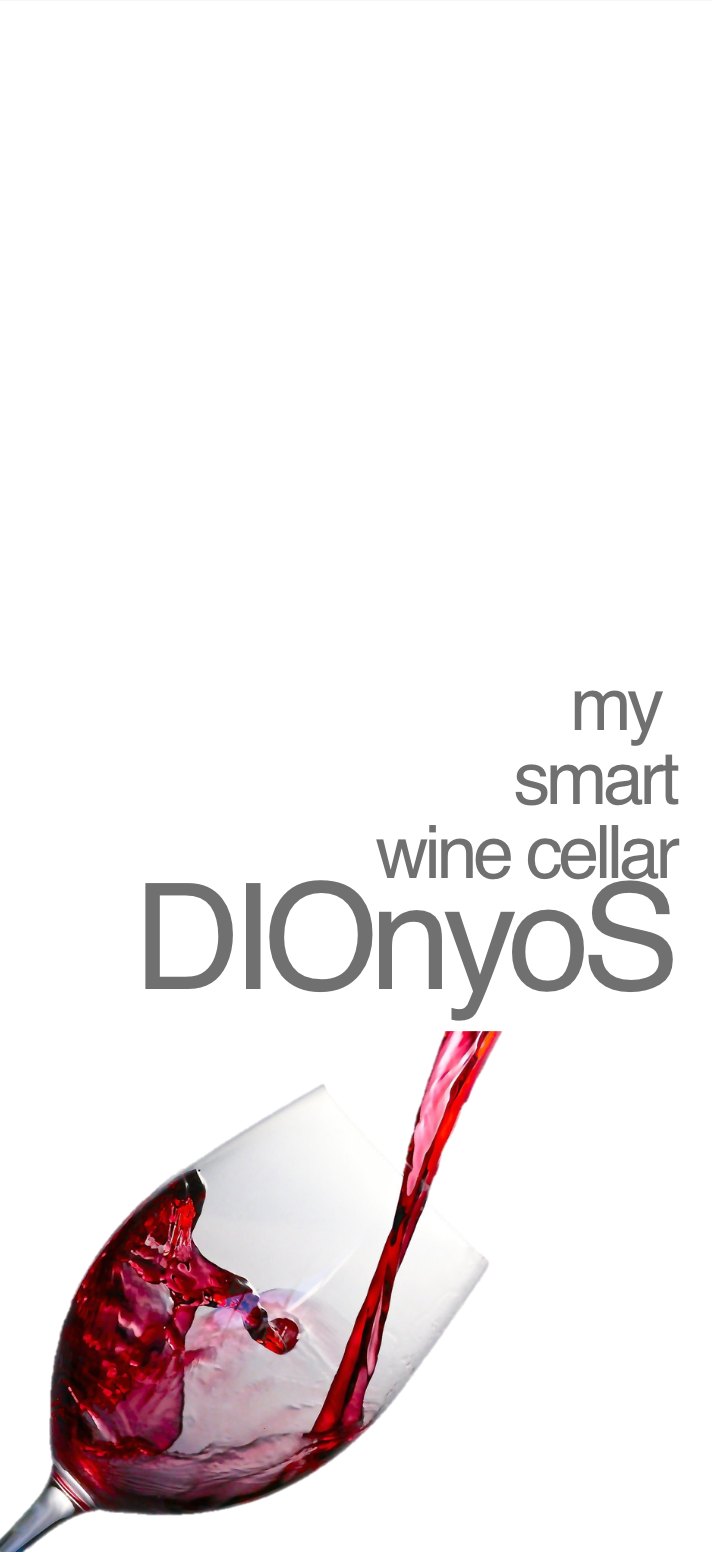
\includegraphics[width=4cm]{firstpage.png}}
    \caption{Welcome Page}
    \centerline{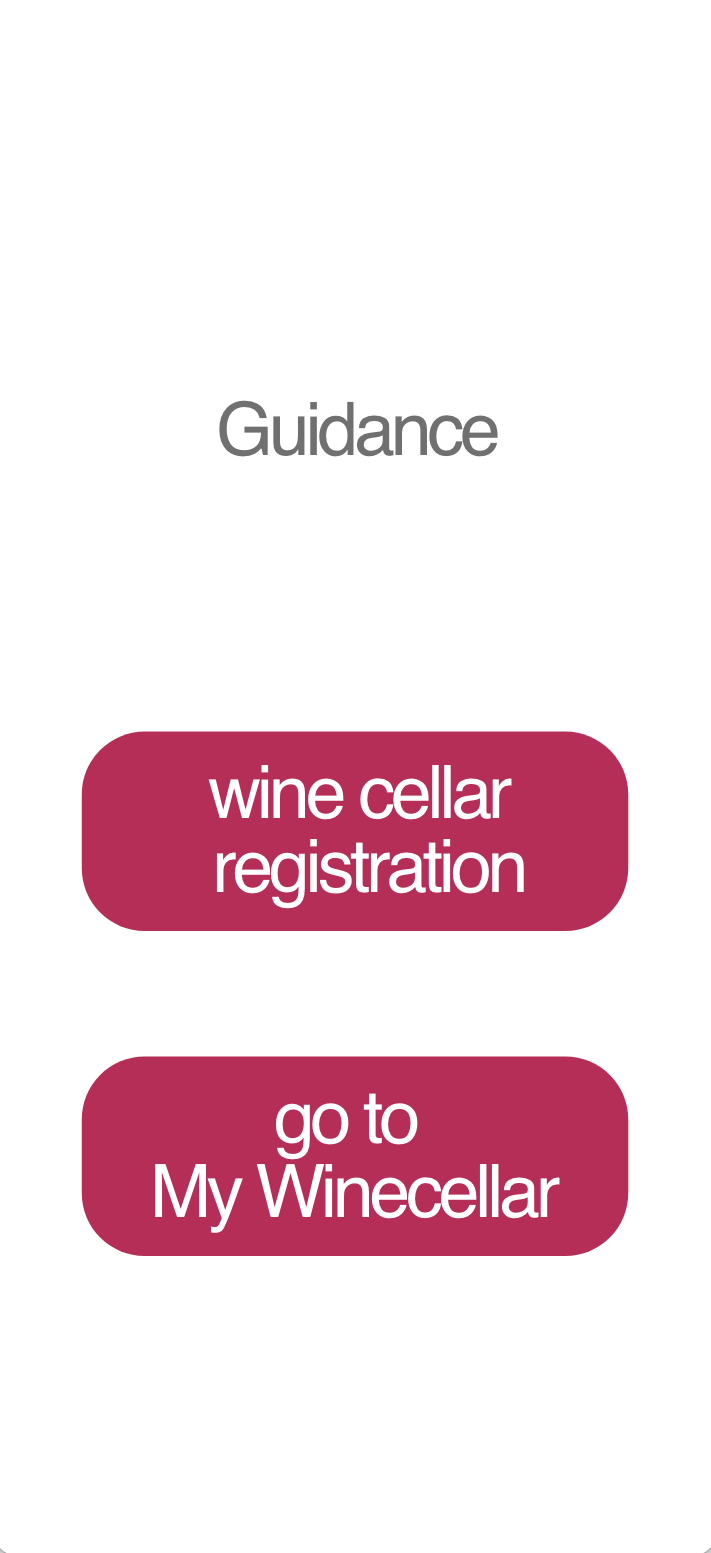
\includegraphics[width=4cm]{guidance.png}}
    \caption{Guidance Page}
\end{figure}
Welcome page is the first screen when downloading this application. If user runs the application, welcome page, which is consisted of ‘Wine cellar registration’ button and ‘go to My Wine cellar’ button.
\begin{enumerate}
    \item \textit{\textbf{Wine cellar registration [Fig.IV-A.3 $\sim$ 4]}}\\
    \begin{figure}[htb!]
        \centerline{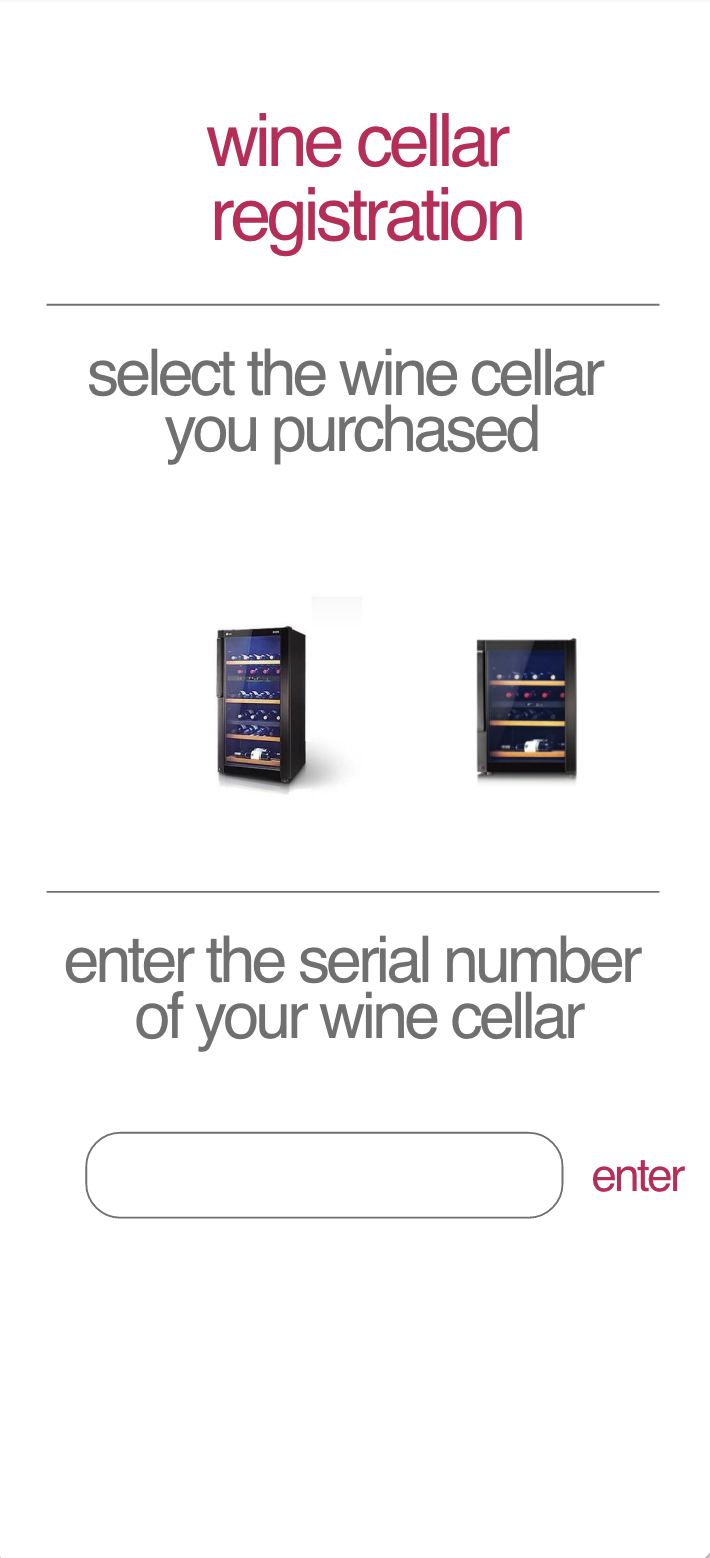
\includegraphics[width=4cm]{winecellarregi.png}}
        \caption{Wine Cellar Registration}
    \end{figure}
    Wine cellar registration button is for user who is first in ‘DIOnyoS’ application and who wants to register another wine cellar in ‘DIOnyoS’. When user press this button, user has to select the wine cellar which he purchased from horizontal scroll. And then user has to enter the serial number of the wine cellar. [Fig.IV-A.3]\\
    \begin{figure}[htb!]
        \centerline{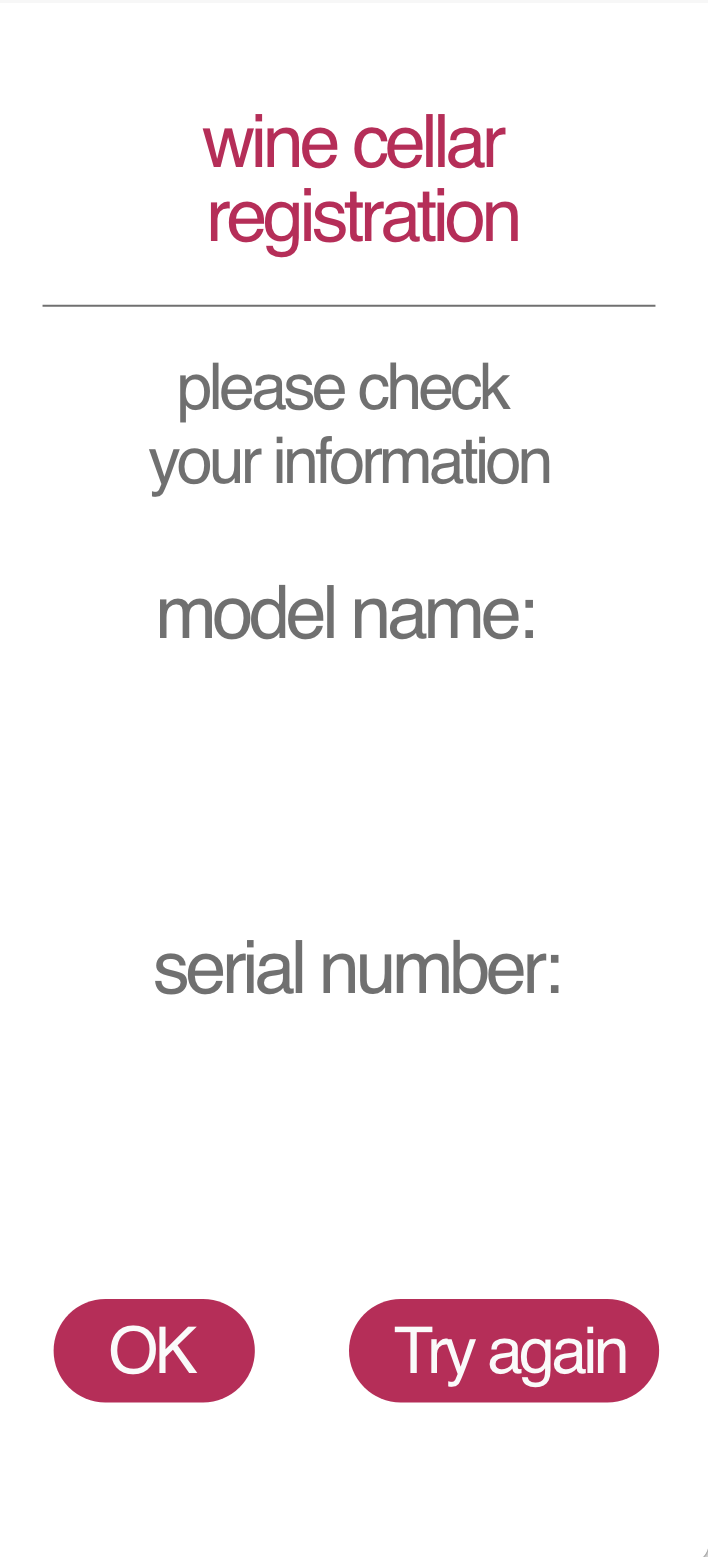
\includegraphics[width=4cm]{regicheck.png}}
        \caption{Registration Check}
    \end{figure}
    After user ends two steps for wine cellar registration, there will be a page for check. If there isn’t any error in registered information, user will push ‘ok’ button to go to ‘My Wine cellar’, which is main page. Or else, user will push ‘try again’ button to re-enter information for wine cellar registration. [Fig.IV-A.4]
    \item \textit{\textbf{Go to my Wine cellar}}\\
    If user presses this button, user can go to ‘My Wine cellar’, which is main page of application.
\end{enumerate}

\subsection{My Wine cellar (Main page) [Fig.IV-B.1]}
\begin{figure}[htb!]
    \centerline{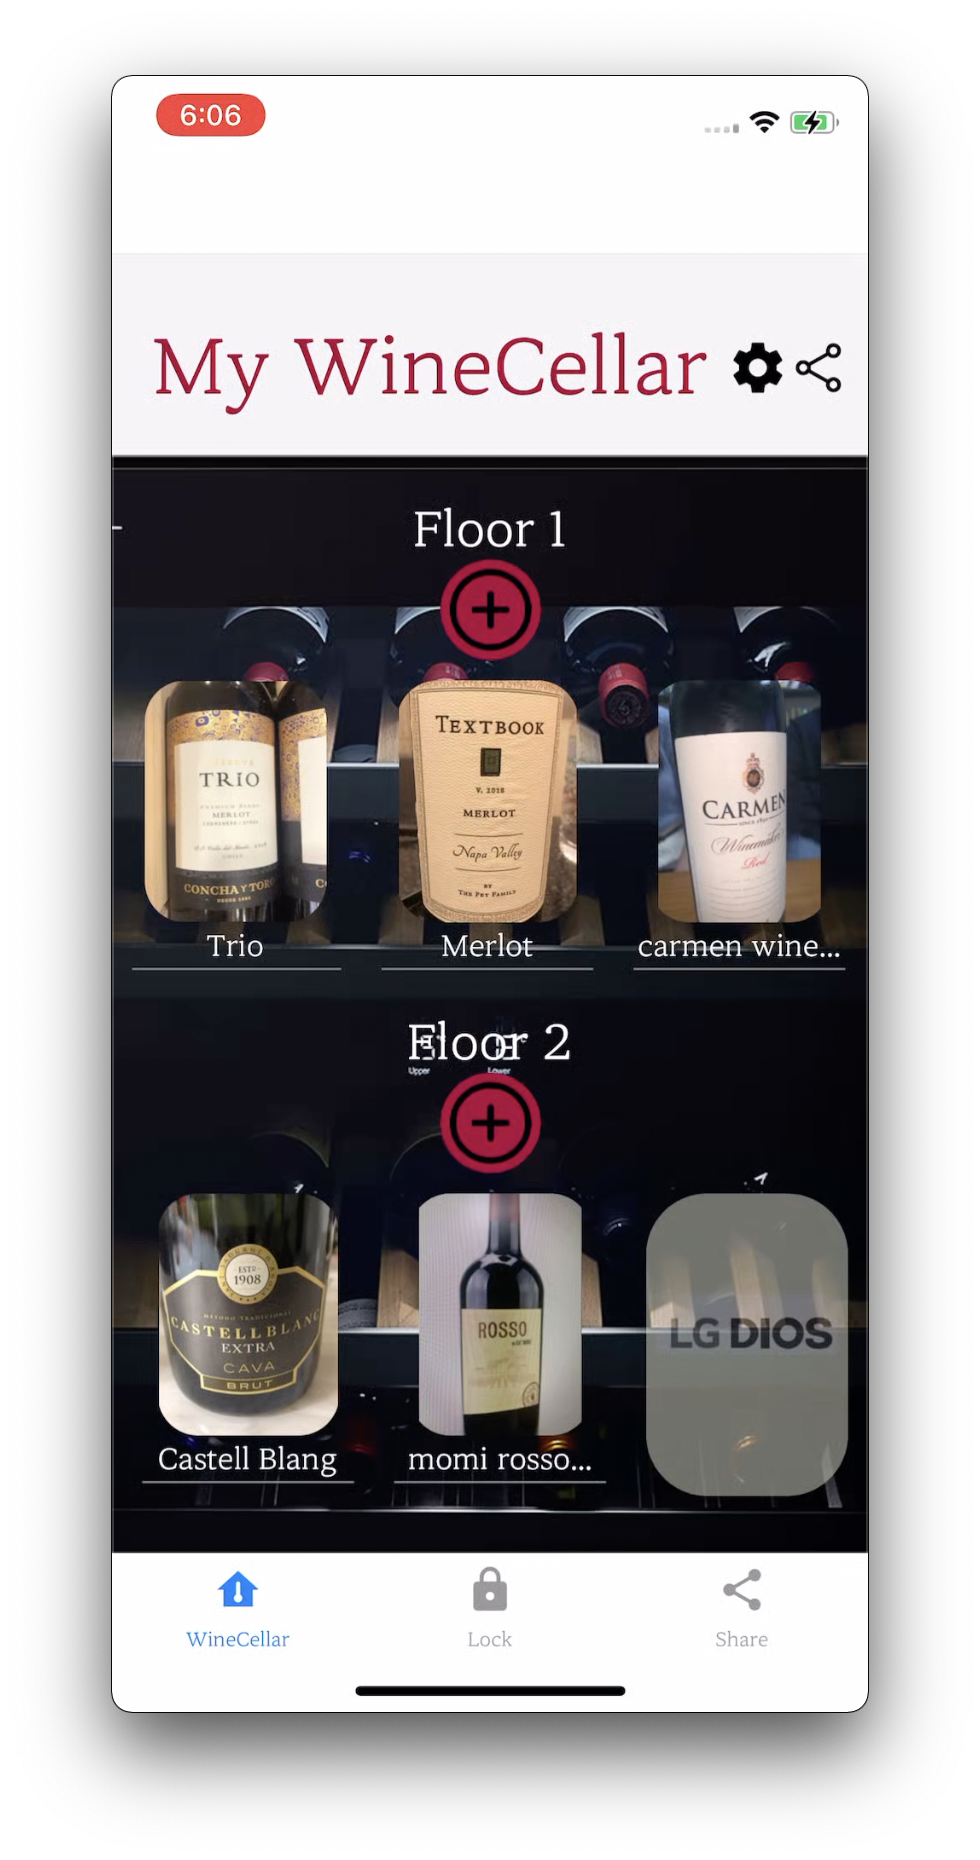
\includegraphics[width=4cm]{mywinece.png}}
    \caption{My Wine Cellar (Main Page)}
\end{figure}
My Wine cellar is the main page of application. My Wine cellar is virtual wine cellar, which shows image of registered wine label in application. Wine cellar is consisted of 4 floors. As there is difference in the size of wine cellar, main page lets user to see wine by scrolling rows.

\begin{enumerate}
    \item \textit{Navigation bar}\\
    Navigation bar is consisted of 4 icons, plus, lock, alarm and share.
    \begin{enumerate}
        \item \textit{\textbf{Wine registration} (Plus icon) [Fig.IV-B.2 $\sim$ 6]}\\  
        When user presses Plus icon, user starts wine registration step.
        \begin{enumerate}
            \begin{figure}[htb!]
                \centerline{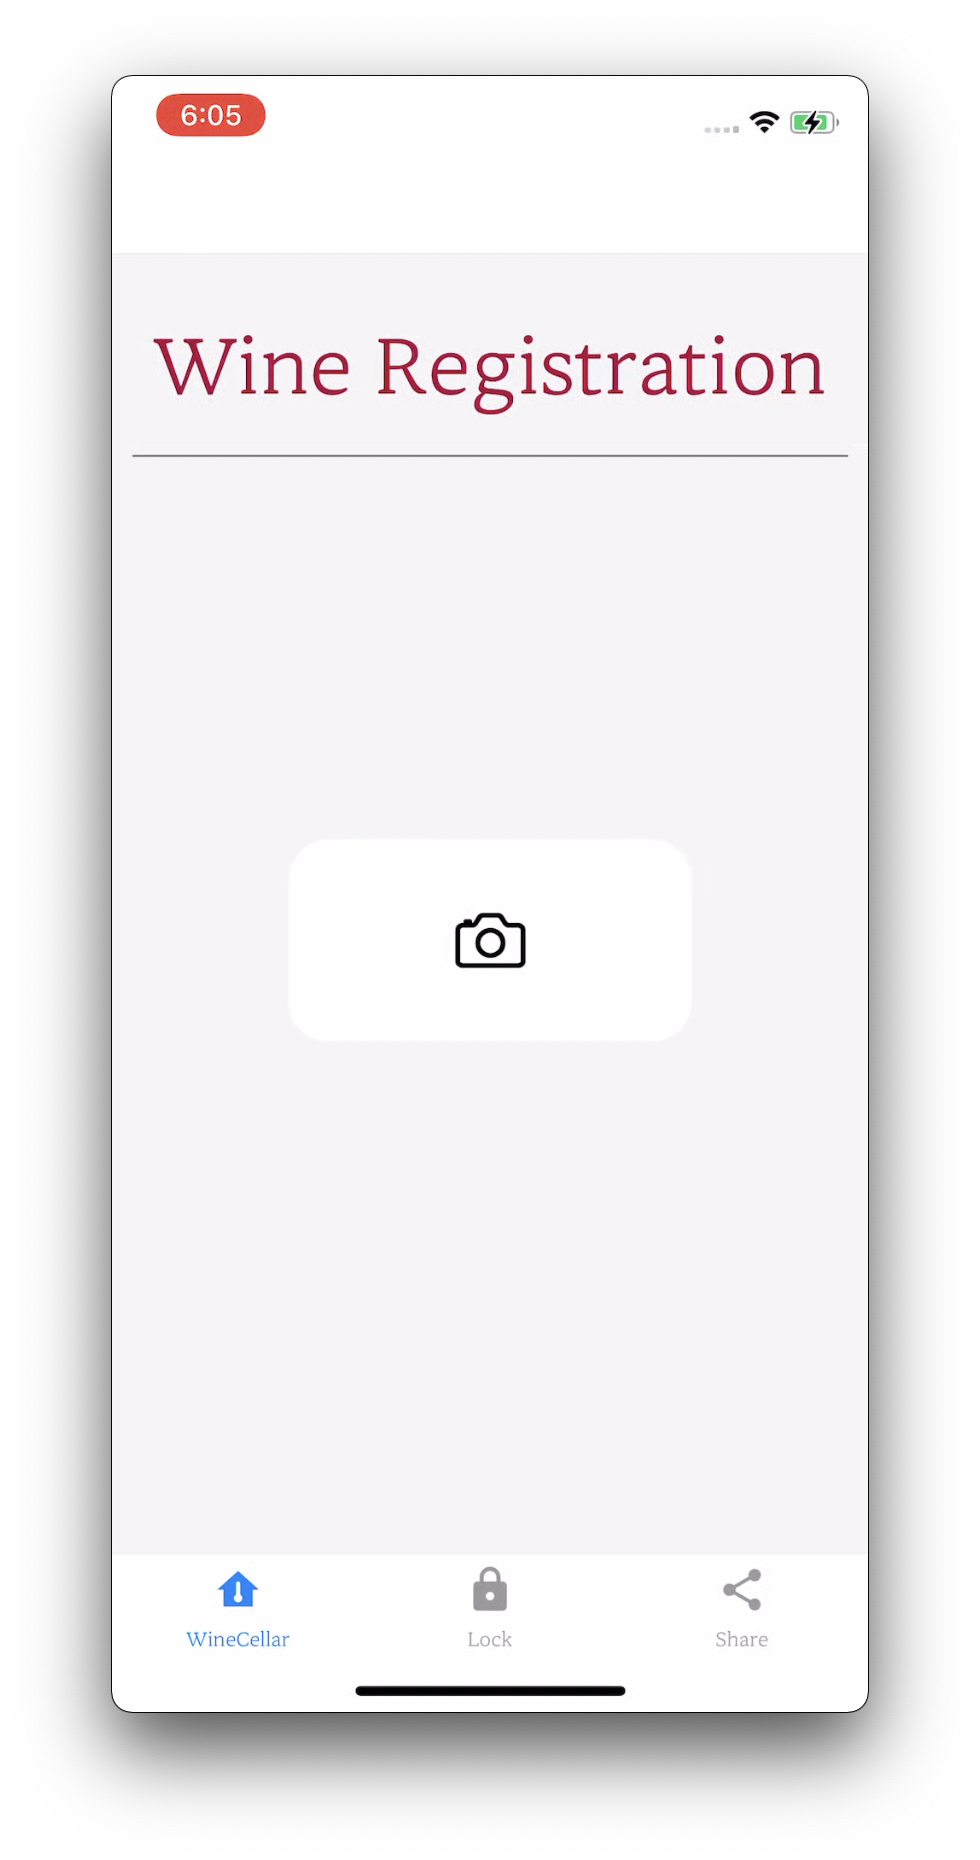
\includegraphics[width=4cm]{camera.png}}
                \caption{Wine Registration using Camera}
                \centerline{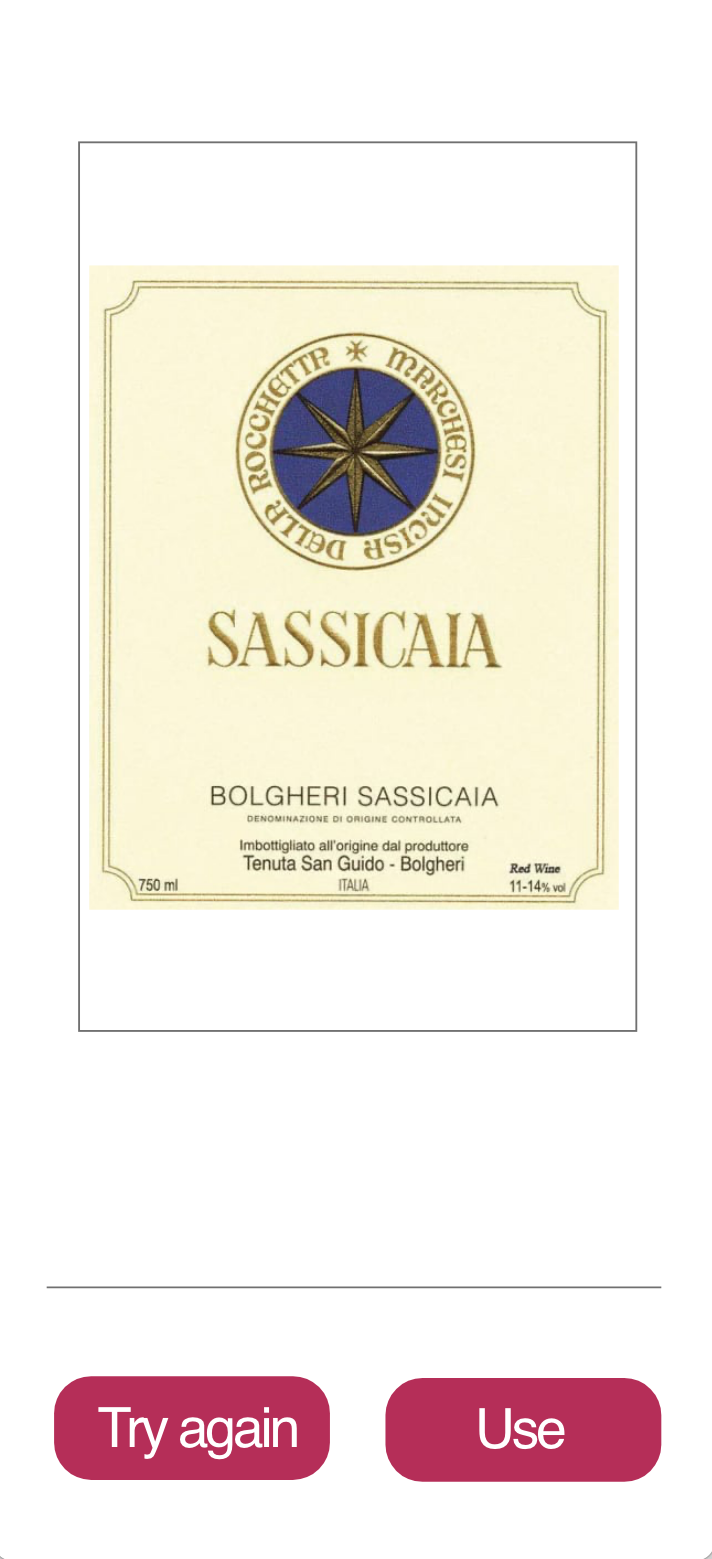
\includegraphics[width=4cm]{photo.png}}
                \caption{Wine Label taken by Camera}
            \end{figure}
            \item User has to open camera application. After taking photo of wine label, user needs to determine whether to use the photo. If user presses ‘try again’ button, user goes to camera application again. Or else, user presses ‘use’ button, user starts wine registration step. [Fig.IV-B.2 \& 3]
            \begin{figure}[htb!]
                \centerline{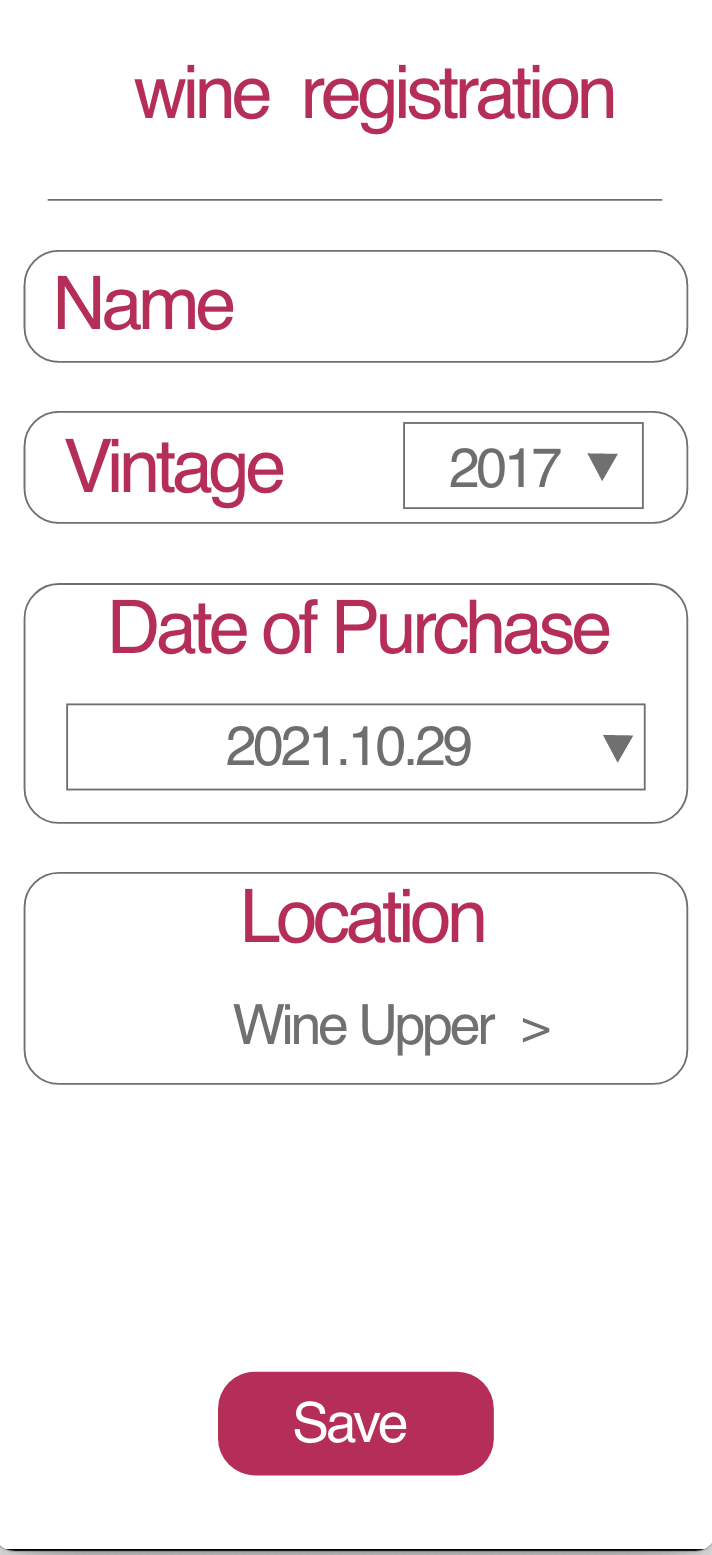
\includegraphics[width=4cm]{regiinfo.png}}
                \caption{Information of Wine taken by Camera}
                \centerline{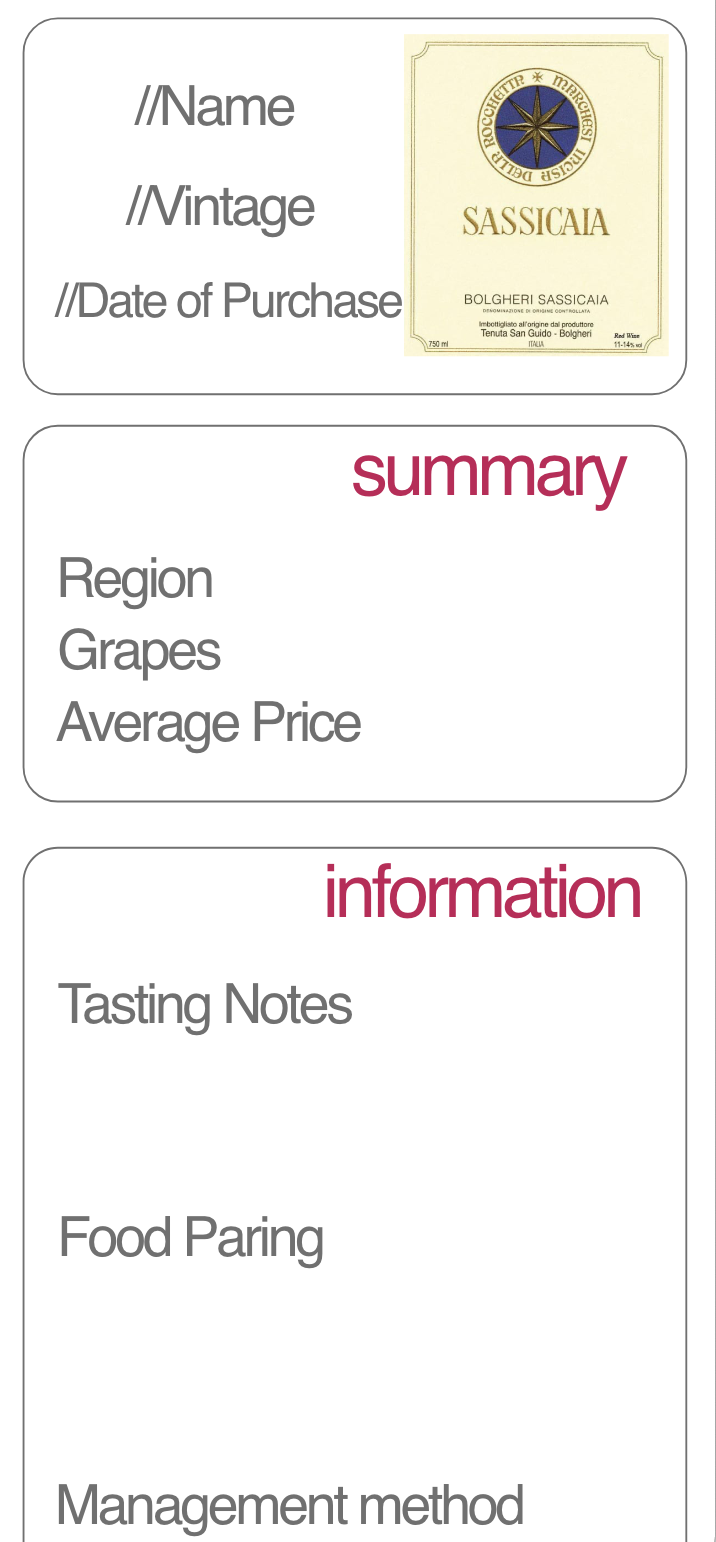
\includegraphics[width=4cm]{wineinfo.png}}
                \caption{Information of Wine}
            \end{figure}
            \item User starts wine registration step by step. Name of wine will be automatically completed by getting name from scanned-wine label database. But user needs to save vintage and date of purchase. Also, user needs to save location of wine, such as wine upper, wine lower. [Fig.IV-B.4 \& 5]
            \begin{figure}[htb!]
                \centerline{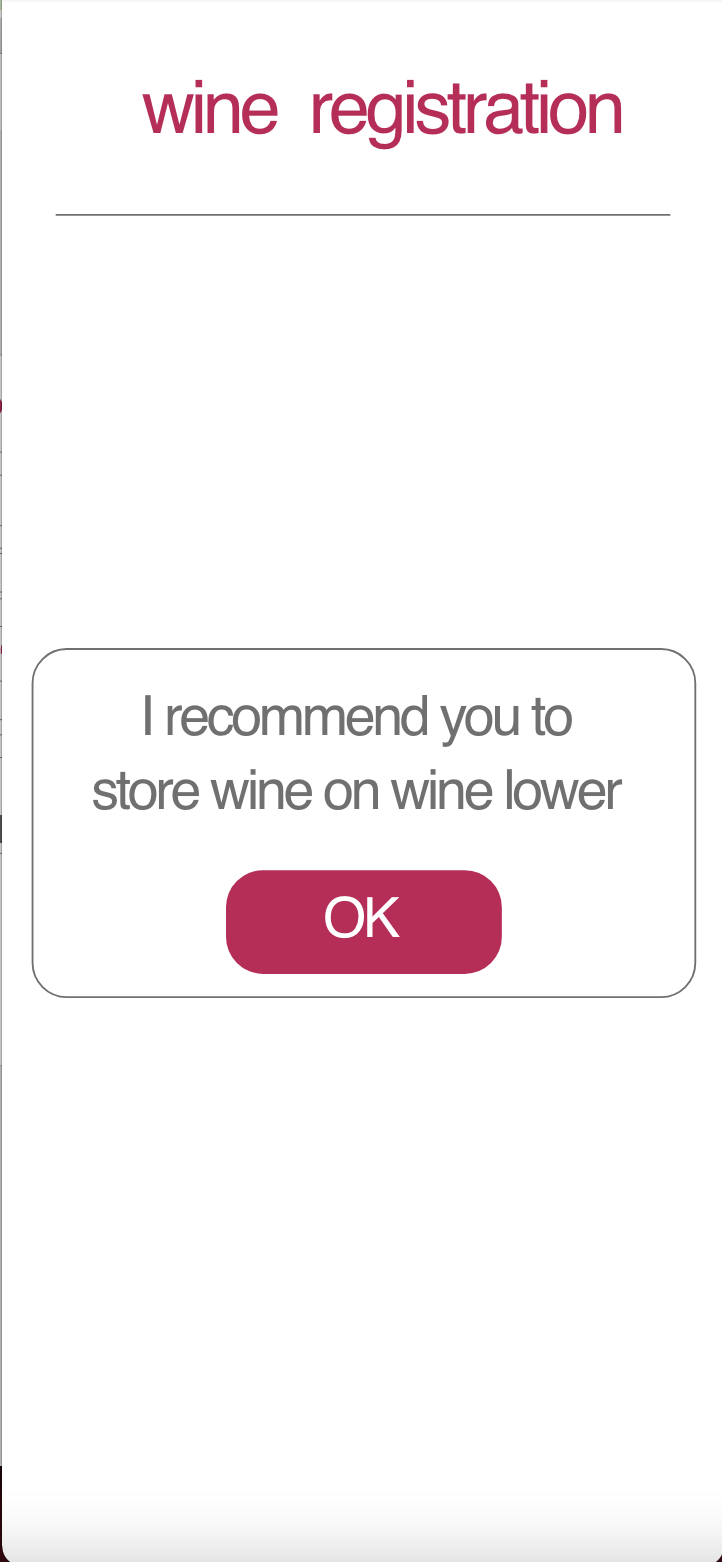
\includegraphics[width=4cm]{infocheck.png}}
                \caption{Checking Information}
            \end{figure}
            \item When user saves these information, pop up window may appear to user. If user saves wine in appropriate floor. [Fig.IV-B.6] \\
        \end{enumerate}
        
        \item \textit{\textbf{Wine cellar Lock} (Lock icon) [Fig.IV-B.7]}\\
        \begin{figure}[htb!]
            \centerline{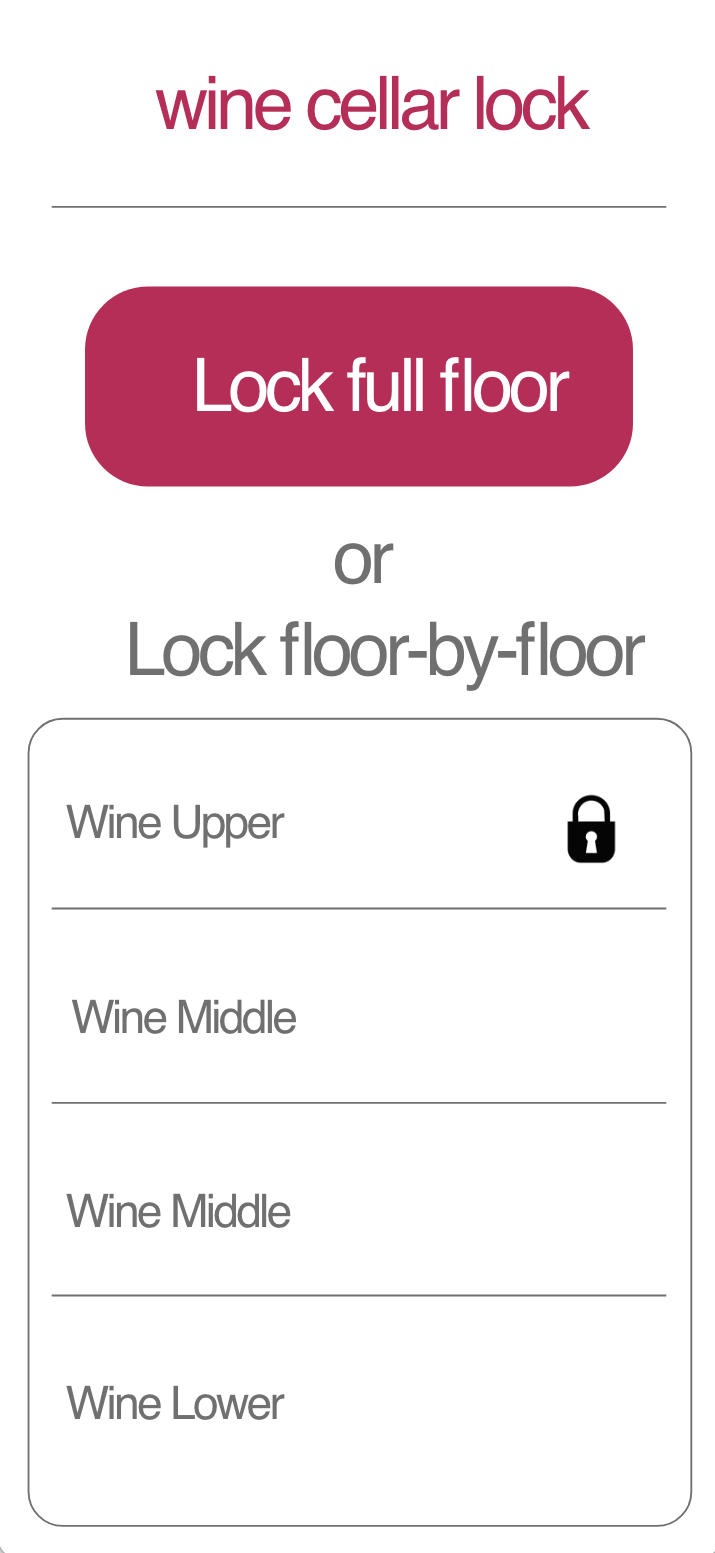
\includegraphics[width=4cm]{lock.png}}
            \caption{Wine Cellar Lock}
        \end{figure}
        When user clicks lock icon, user goes to ‘wine cellar lock’. If user wants to lock full floor, user can click ‘lock full floor button’. Or else, user can lock floor by floor by clicking each lock button.\\
        
        \item \textit{\textbf{Wine Recommendation} (Alarm icon) [Fig.IV-B.8 $\sim$ 16]}\\
        \begin{figure}[htb!]
            \centerline{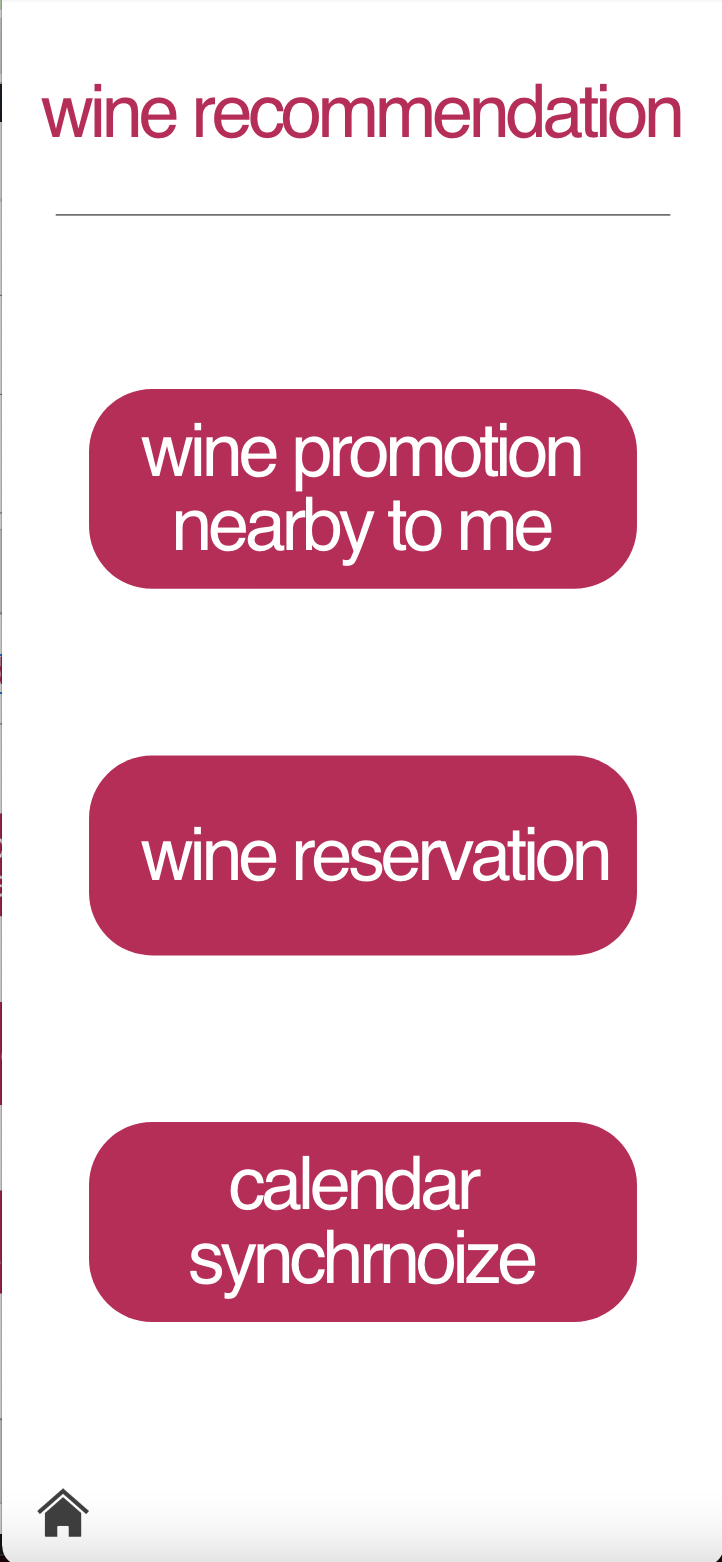
\includegraphics[width=4cm]{winerec.png}}
            \caption{Wine Recommendation}
        \end{figure}
        On the wine recommendation page, users can go to pages that check nearby wine-related events (e.g., discounts), get information about 'nearby wine shops', 'buy wine or make reservations', and 'recommend wine which fits in with their schedules'. 
        \begin{enumerate}
            \item \textit{Wine promotion nearby to me [Fig.IV-B.9 \& 10]}
            \begin{enumerate}
                \begin{figure}[htb!]
                    \centerline{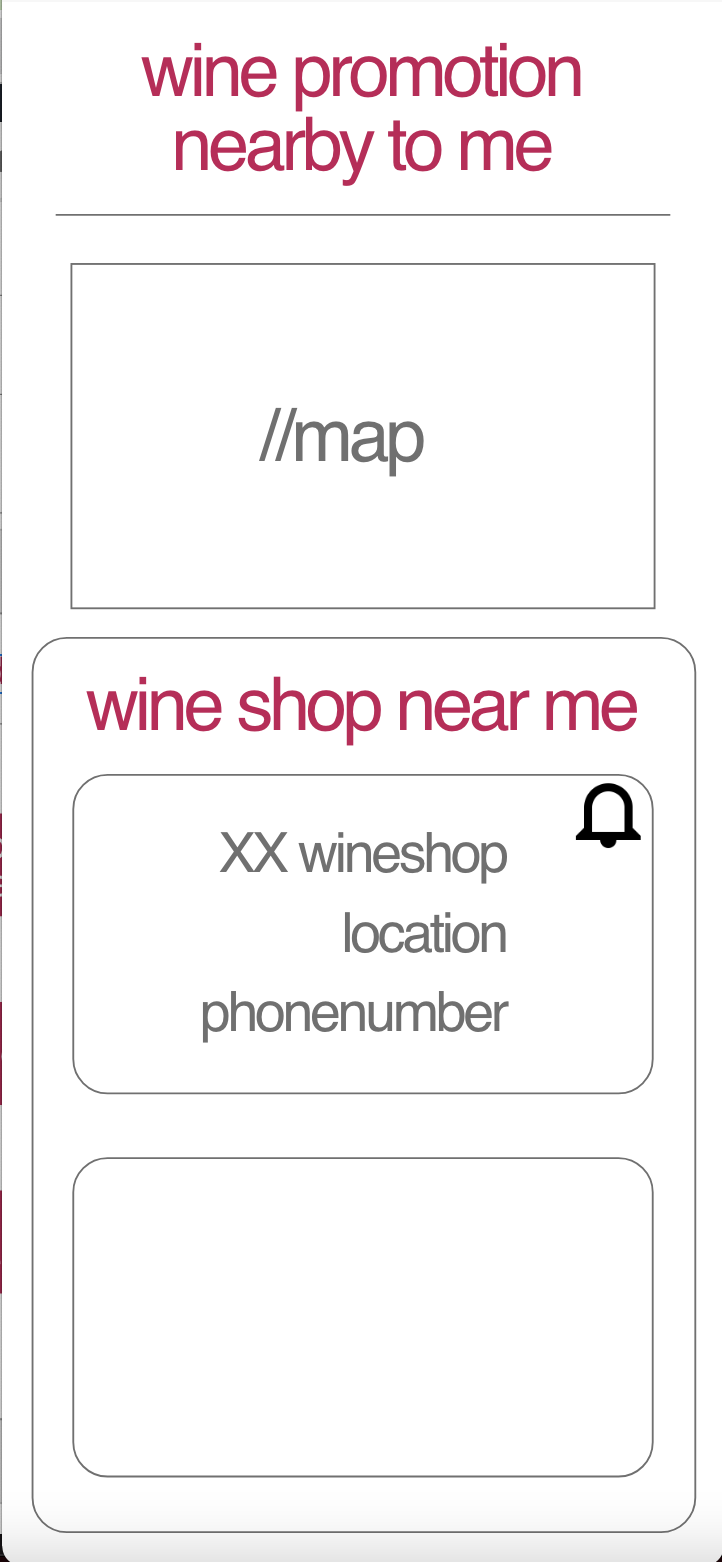
\includegraphics[width=4cm]{winepromo.png}}
                    \caption{Wine Promotion}
                \end{figure}
                \item The application requests the user's location information. If the user allows the request, the map displays wine promotion around the user. 
                \item The 'wine shop nearby to me' view under the 'map' view displays wine shops around the user. Users can set alarms for each wine shop by clicking the bell icon on the top right. If an event or promotion is held at a wine shop with an alarm set, the application sends a notification to the user. 
                \begin{figure}[htb!]
                    \centerline{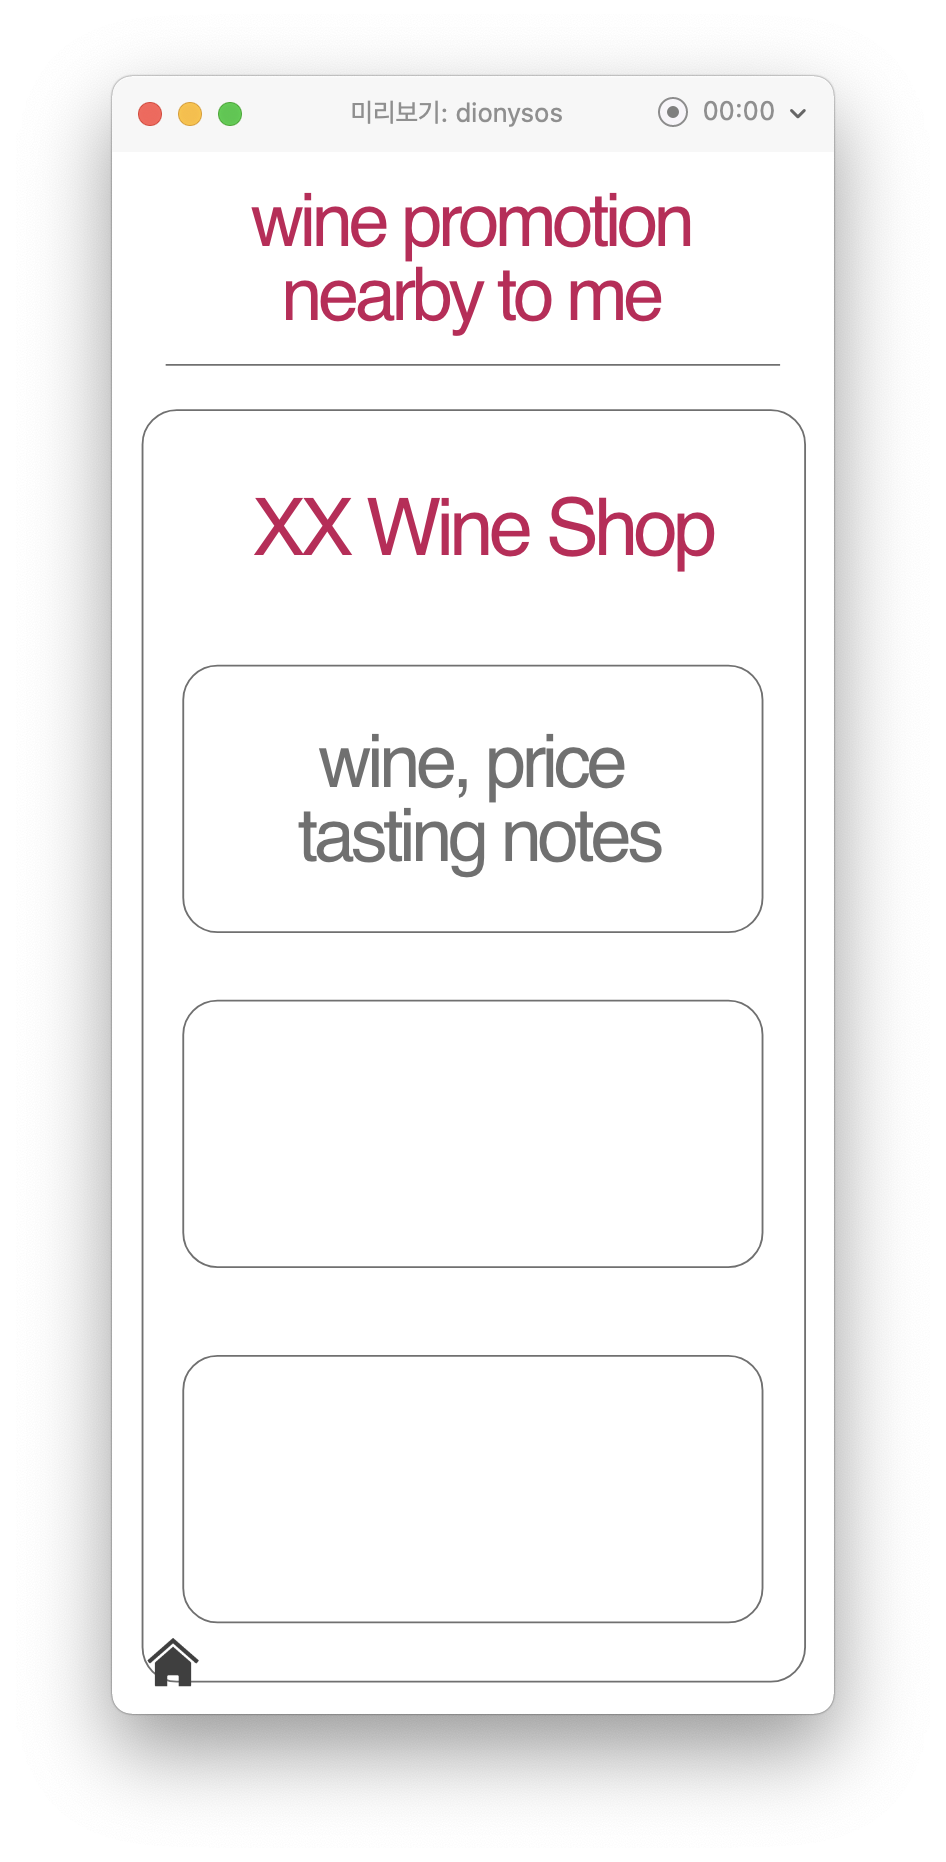
\includegraphics[width=4cm]{winepromoalarm.png}}
                    \caption{Alarm of Wine Promotion}
                \end{figure}
                \item When the user clicks the notification, wines corresponding to the event at the wine shop are displayed. The app shows the name, price, and testing notes of the wine.
            \end{enumerate}
            
            \item \textit{Wine reservation [Fig.IV-B 11 $sim$ 13]}\\
            On the Wine Reservation page, users can search for and reserve the wine they want to purchase. 
            \begin{enumerate}
                \begin{figure}[htb!]
                    \centerline{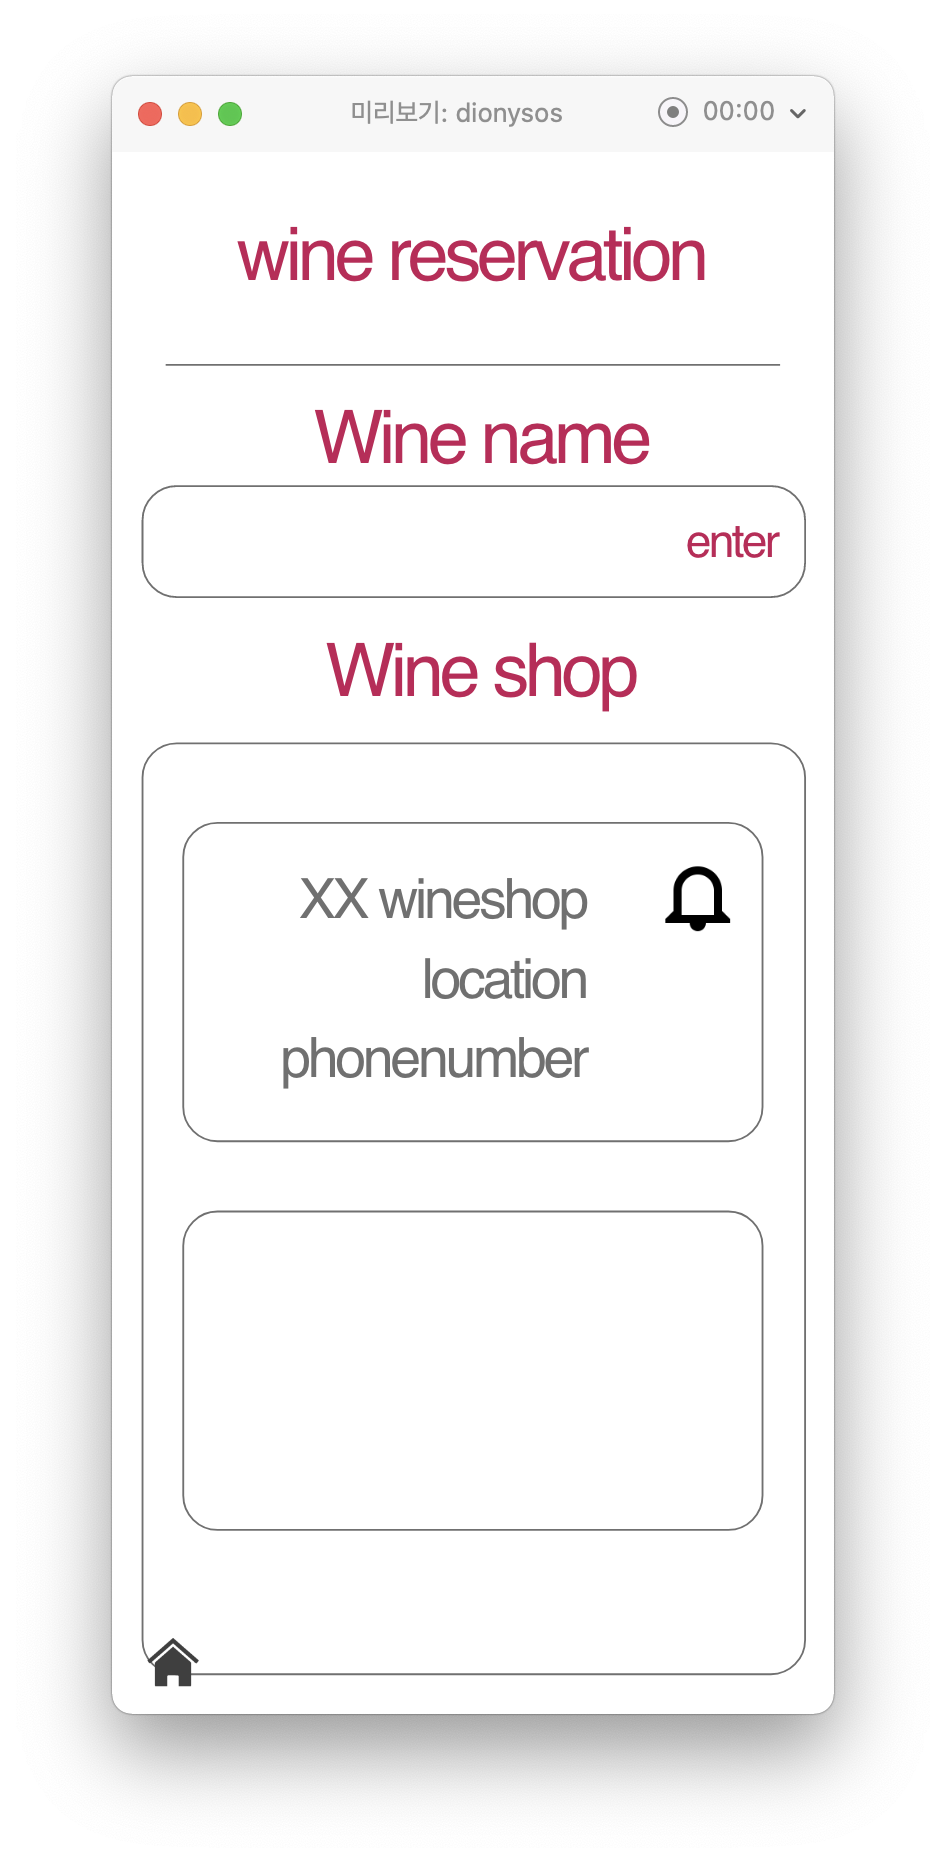
\includegraphics[width=4cm]{wineres.png}}
                    \caption{Wine Reservation}
                \end{figure}
                \item The user can search for wine by entering the name of the wine. When the user writes the name of the wine and presses the enter button, the app shows several shops where wine entered by the user can be purchased.\\
                The user can press the bell button on the upper right in each wine shop view to receive a notification whenever the wine he or she wants becomes available for purchase. App sends notification if the wine user wants has arrived at the wine shop. [Fig.IV-B.11]
                \item Alarm [Fig.IV-B.12]\\
                \begin{figure}[htb!]
                    \centerline{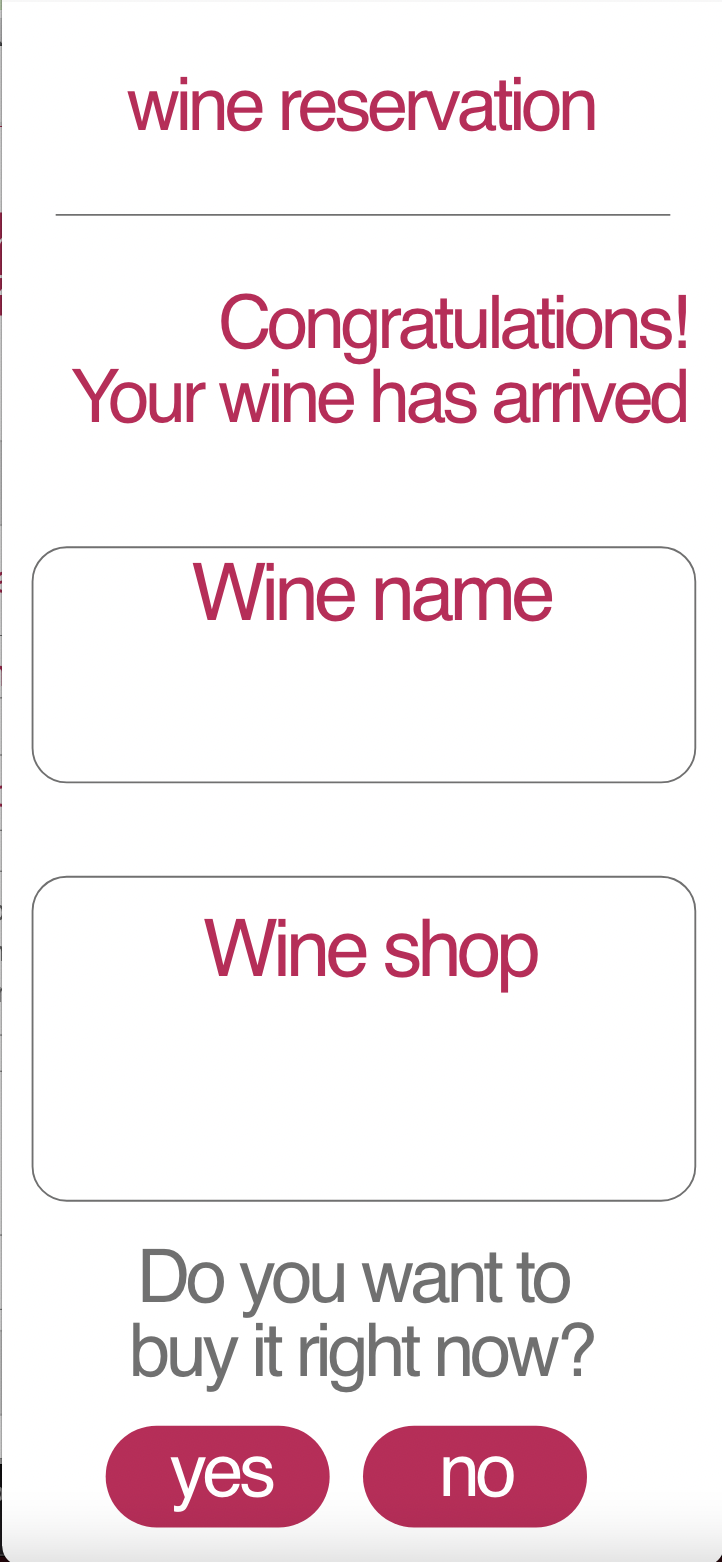
\includegraphics[width=4cm]{winearrive.png}}
                    \caption{Arrival of Wine}
                \end{figure}
                When wine that user wants arrives at the wine shop where the user presses the bell button and becomes available, the app sends a notification to the user. When the user clicks the notification, it goes to the Congratulation page. On the Congratulation page, users can see the name of the wine and the store they reserved, and the question of whether to purchase it 'right now'.\\
                \item Reservation [Fig.IV-B.13]\\
                \begin{figure}[htb!]
                    \centerline{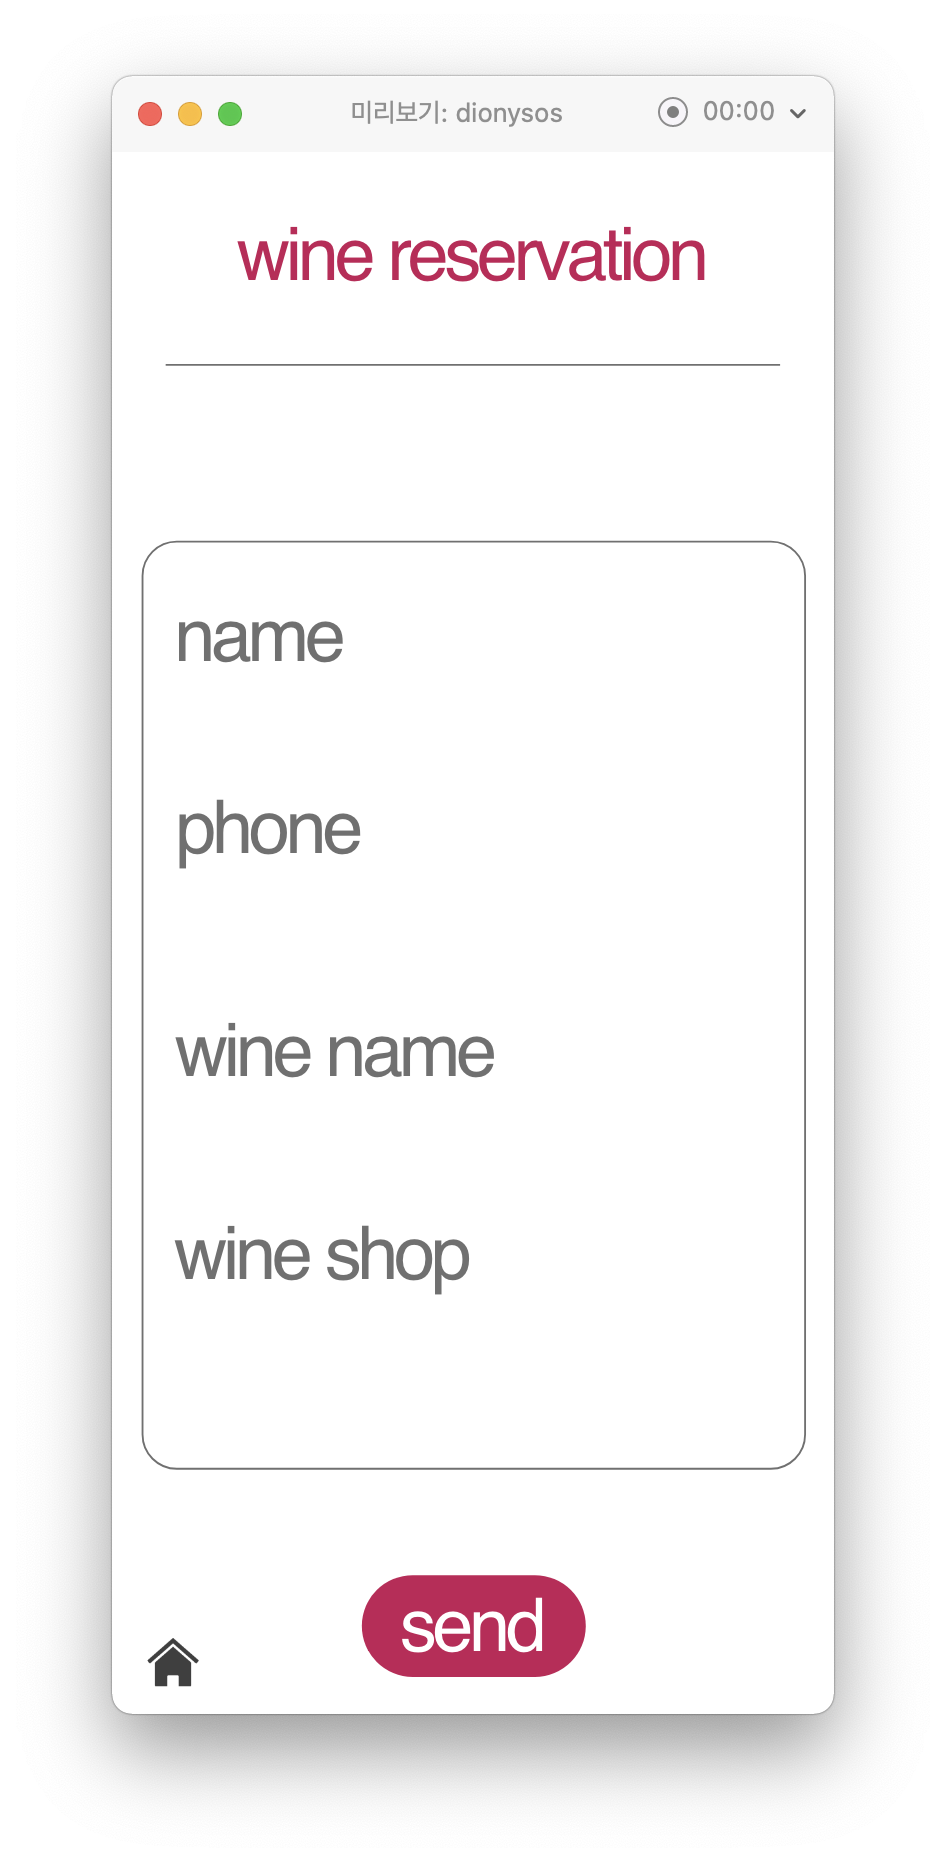
\includegraphics[width=4cm]{winebuy.png}}
                    \caption{Purchasing Wine}
                \end{figure}
                If the user presses yes to show his intention to purchase it right now, go to the 'wine reservation' page. On the 'wine reservation' page, the user writes down his name, phone number, name of wine to purchase, and name of the store to purchase wine and presses the send button. The information pressed here is sent to the corresponding wine store. \\
            \end{enumerate}
            
            \item \textit{Calendar synchronize [Fig.IV-B.14 \& 15]}\\
            \begin{figure}[htb!]
                \centerline{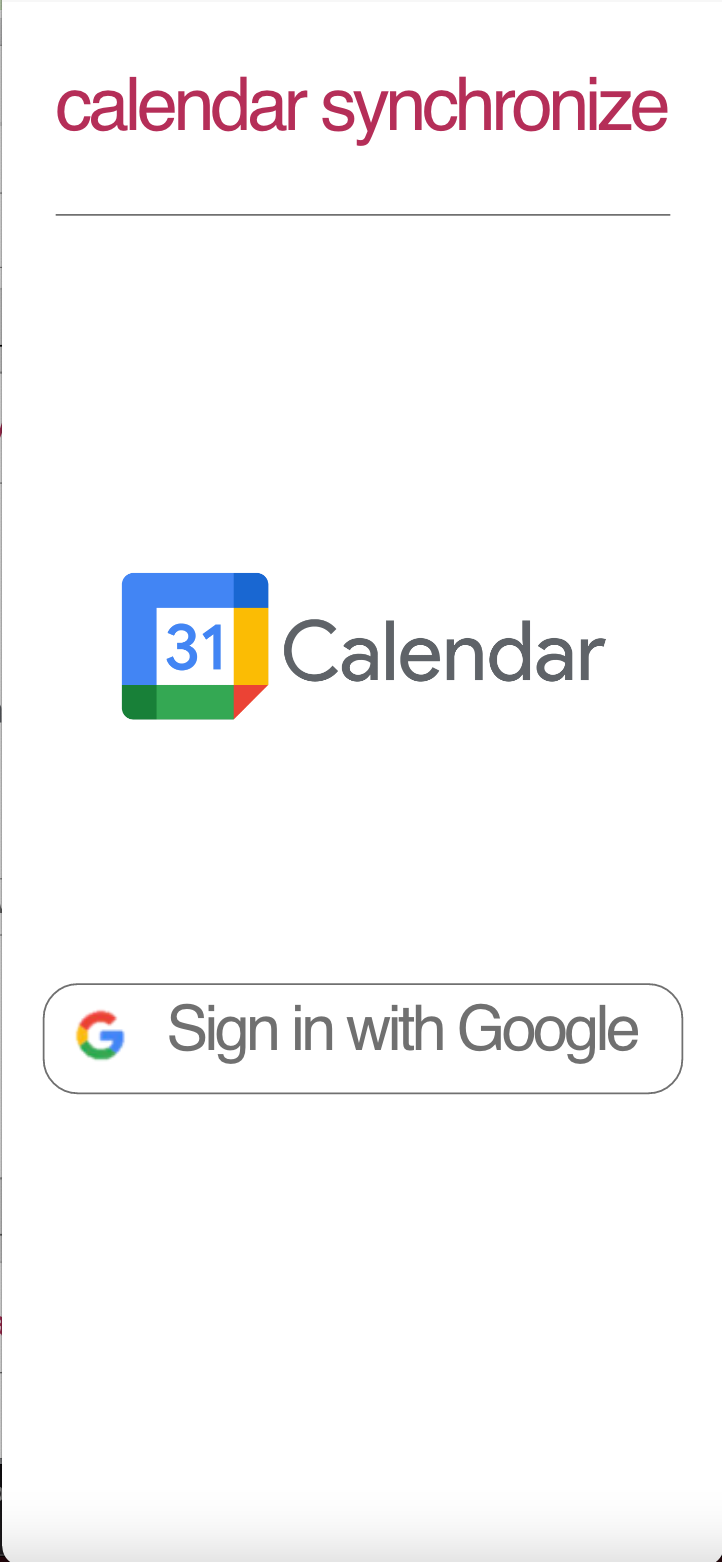
\includegraphics[width=4cm]{calendar.png}}
                \caption{Google Calendar}
                \centerline{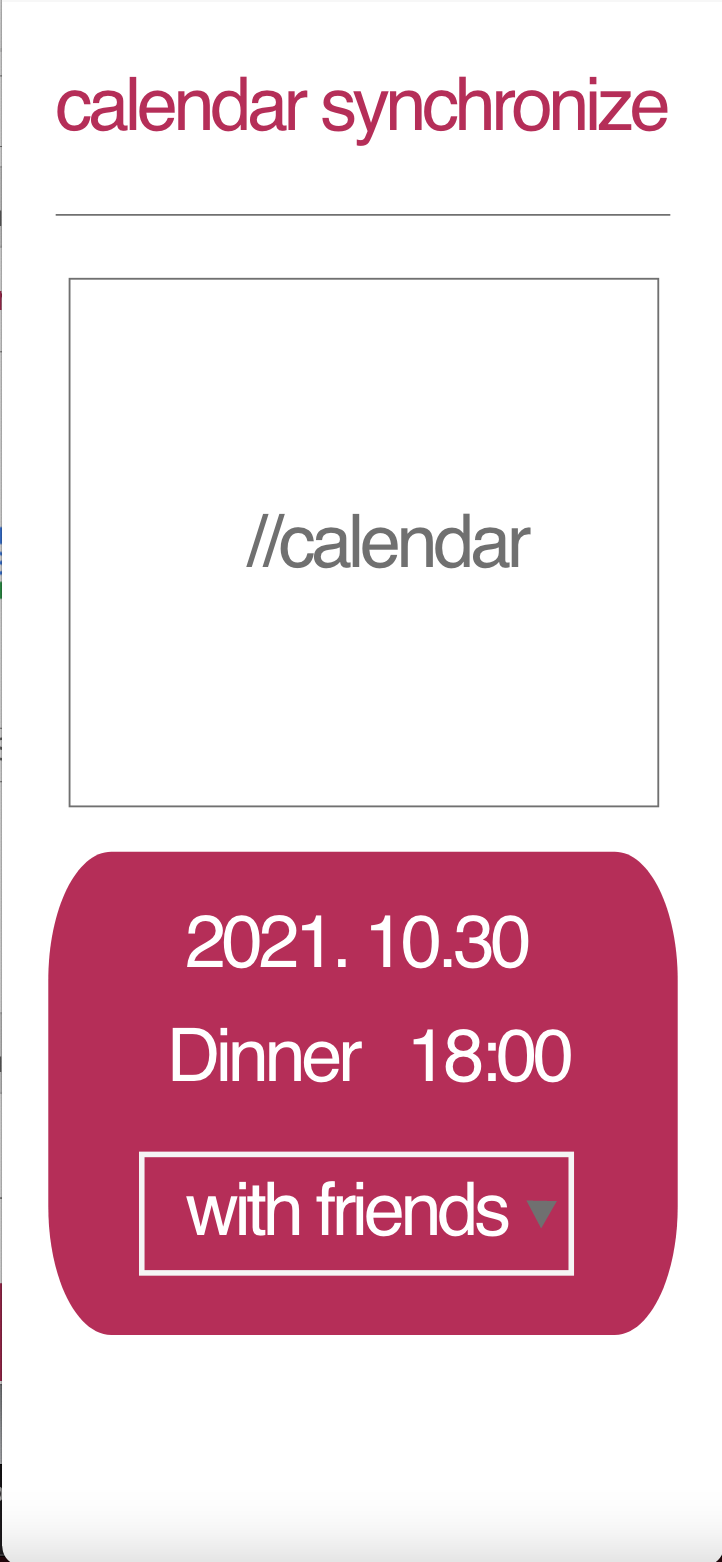
\includegraphics[width=4cm]{calendar2.png}}
                \caption{Calendar}
            \end{figure}
            By logging in with their Google account, users can link this app with their Google Calendar.\\
            Using Google-Calendar-api, the application displays the calendar of current month. When the user clicks on the day with schedule, the schedule of the day is displayed in the view under the calendar. The daily schedule indicates the date and time, the purpose of the schedule (e.g., evening, party), and who users are meeting with.\\
            The app focuses on 'people' who are together that day. The recommended wine depends on who the users are with that day. People who share schedule with users are highlighted with white lines. If the user presses the highlighted part (button), the app goes to the 'wine information' page of the recommended wine.\\
        \end{enumerate}
        
        \item \textit{\textbf{Share} (Share icon) [Fig.IV-B.16 $\sim$ 22]}\\
        \begin{figure}[htb!]
            \centerline{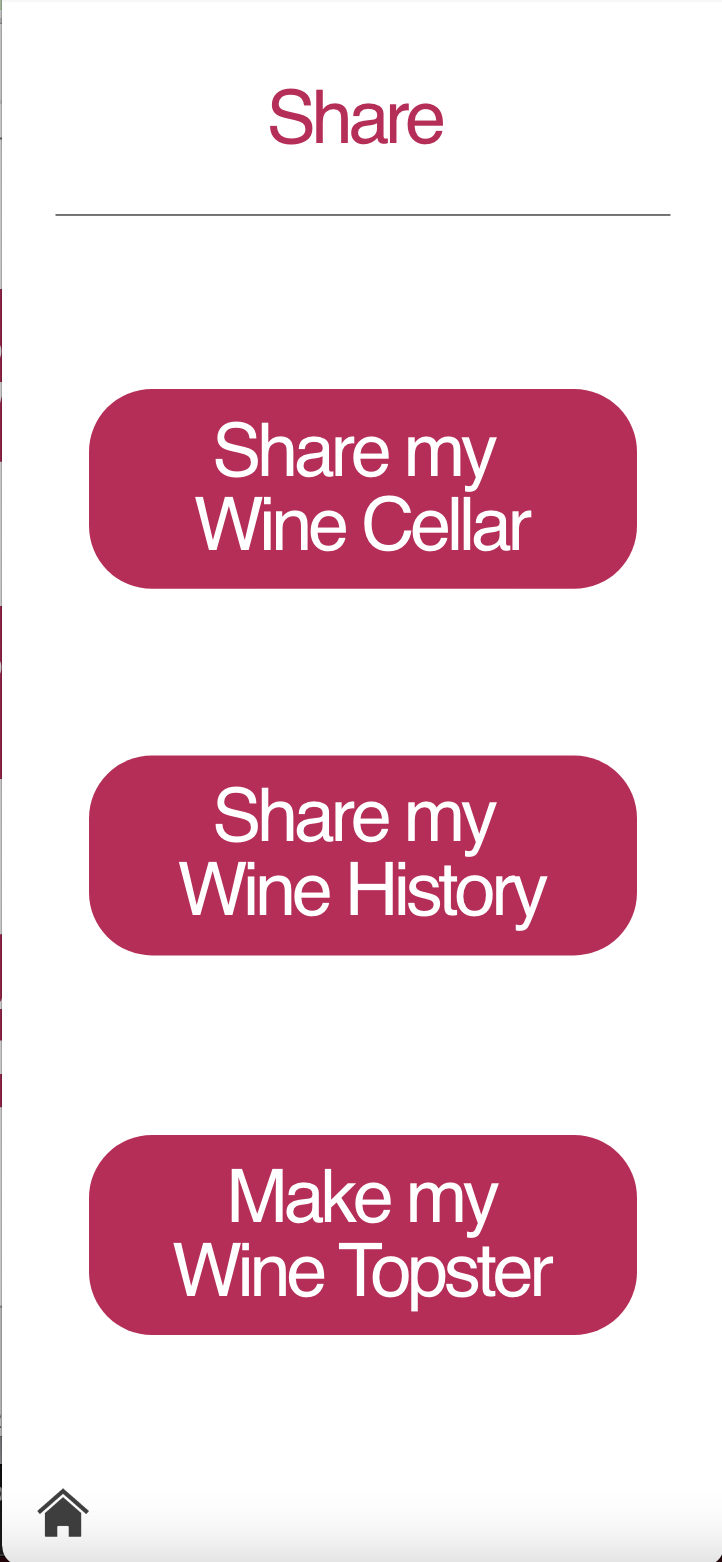
\includegraphics[width=4cm]{share.png}}
            \caption{Share}
        \end{figure}
        Share, which is consisted of ‘Share my Wine cellar’, ‘Share my Wine history’, and ‘Make my Wine Topster’, lets user to share wine-related images in Instagram, Facebook, Twitter and saves images to gallery in common. When user shares these images, hashtag \#LGwinecellar, \#MyWineCellar, and \#DIOnyoS will be automatically completed. And it can lead to promotion of wine cellar and application DIOnyoS.
        \begin{enumerate}
            \item \textit{Share my Wine Cellar [Fig.IV-B.17]}\\
            \begin{figure}[htb!]
                \centerline{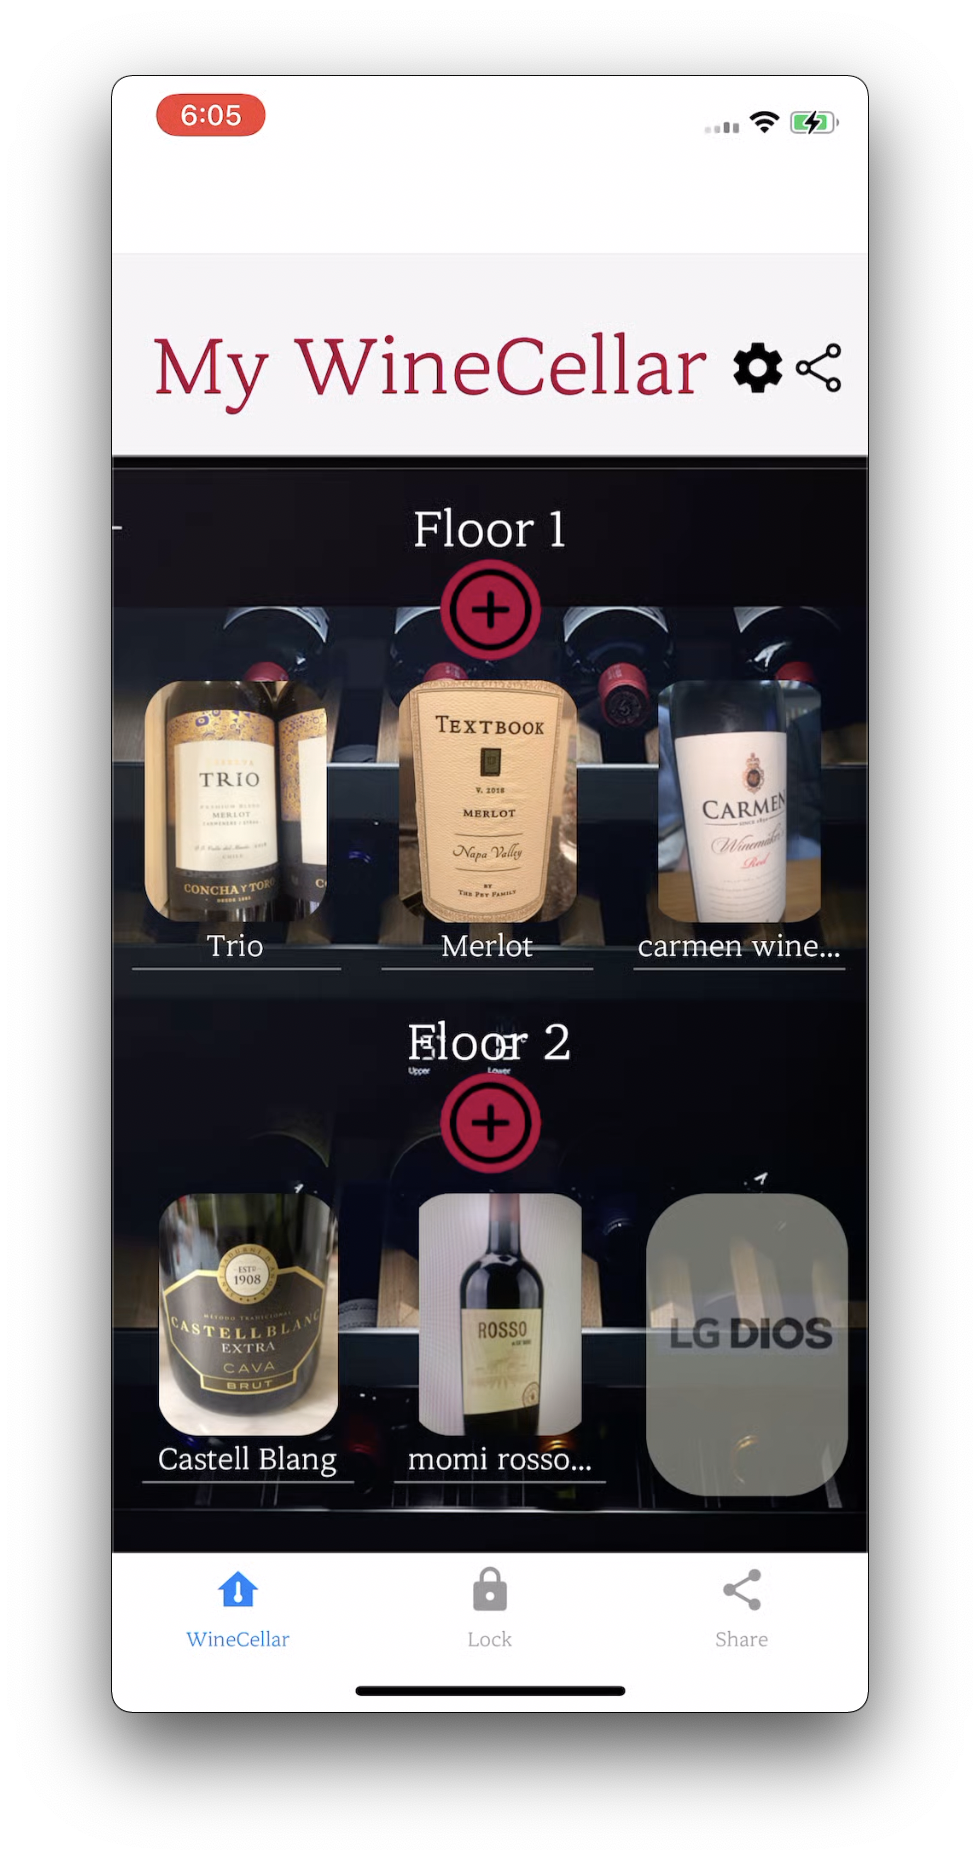
\includegraphics[width=4cm]{sharecel.png}}
                \caption{Share Wine Cellar}
            \end{figure}
            Share my Wine Cellar lets user to take screentshot of ‘My WineCellar’, which is main page.
            \item \textit{Share my Wine History}
            \begin{enumerate}
                \item Cork [Fig.IV-B.18]\\
                \begin{figure}[htb!]
                    \centerline{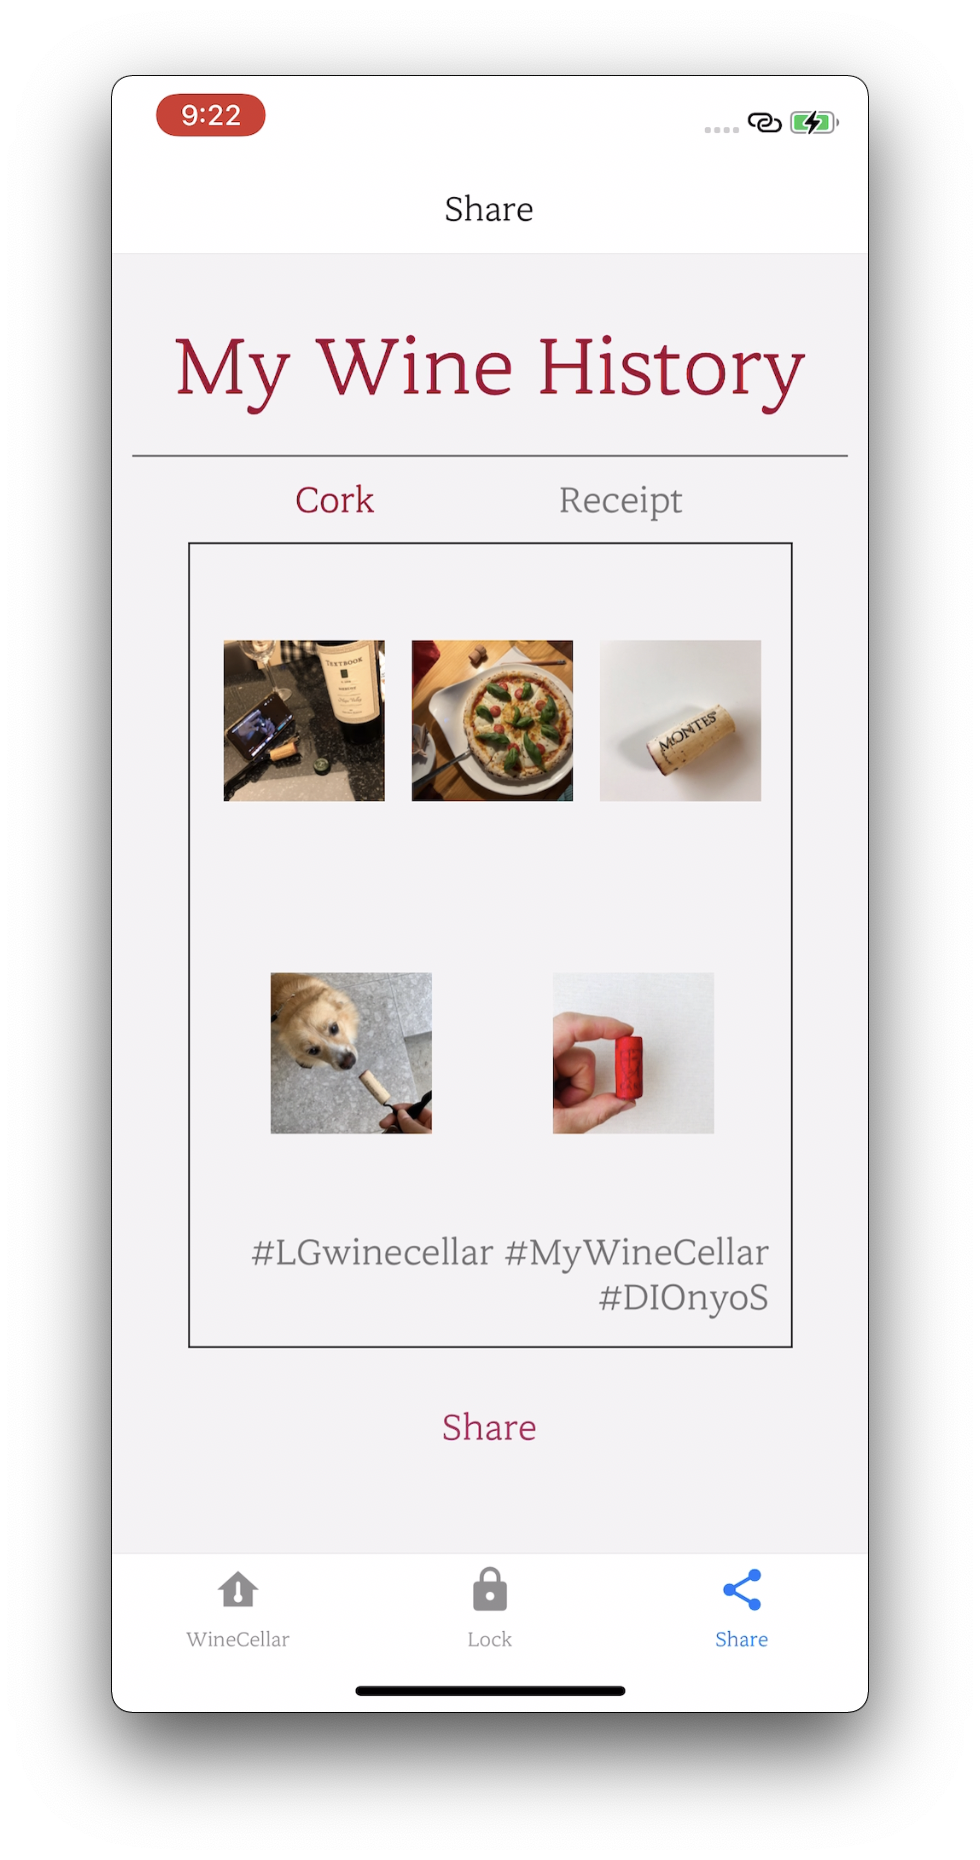
\includegraphics[width=4cm]{sharecork.png}}
                    \caption{Share Cork}
                \end{figure}
                The number of wine which user has drunk until now appears as the images of cork. And it will look like loyalty card. So, the more user drink, the more cork user can collect.
                \item Receipt [Fig.IV-B.19]\\
                \begin{figure}[htb!]
                    \centerline{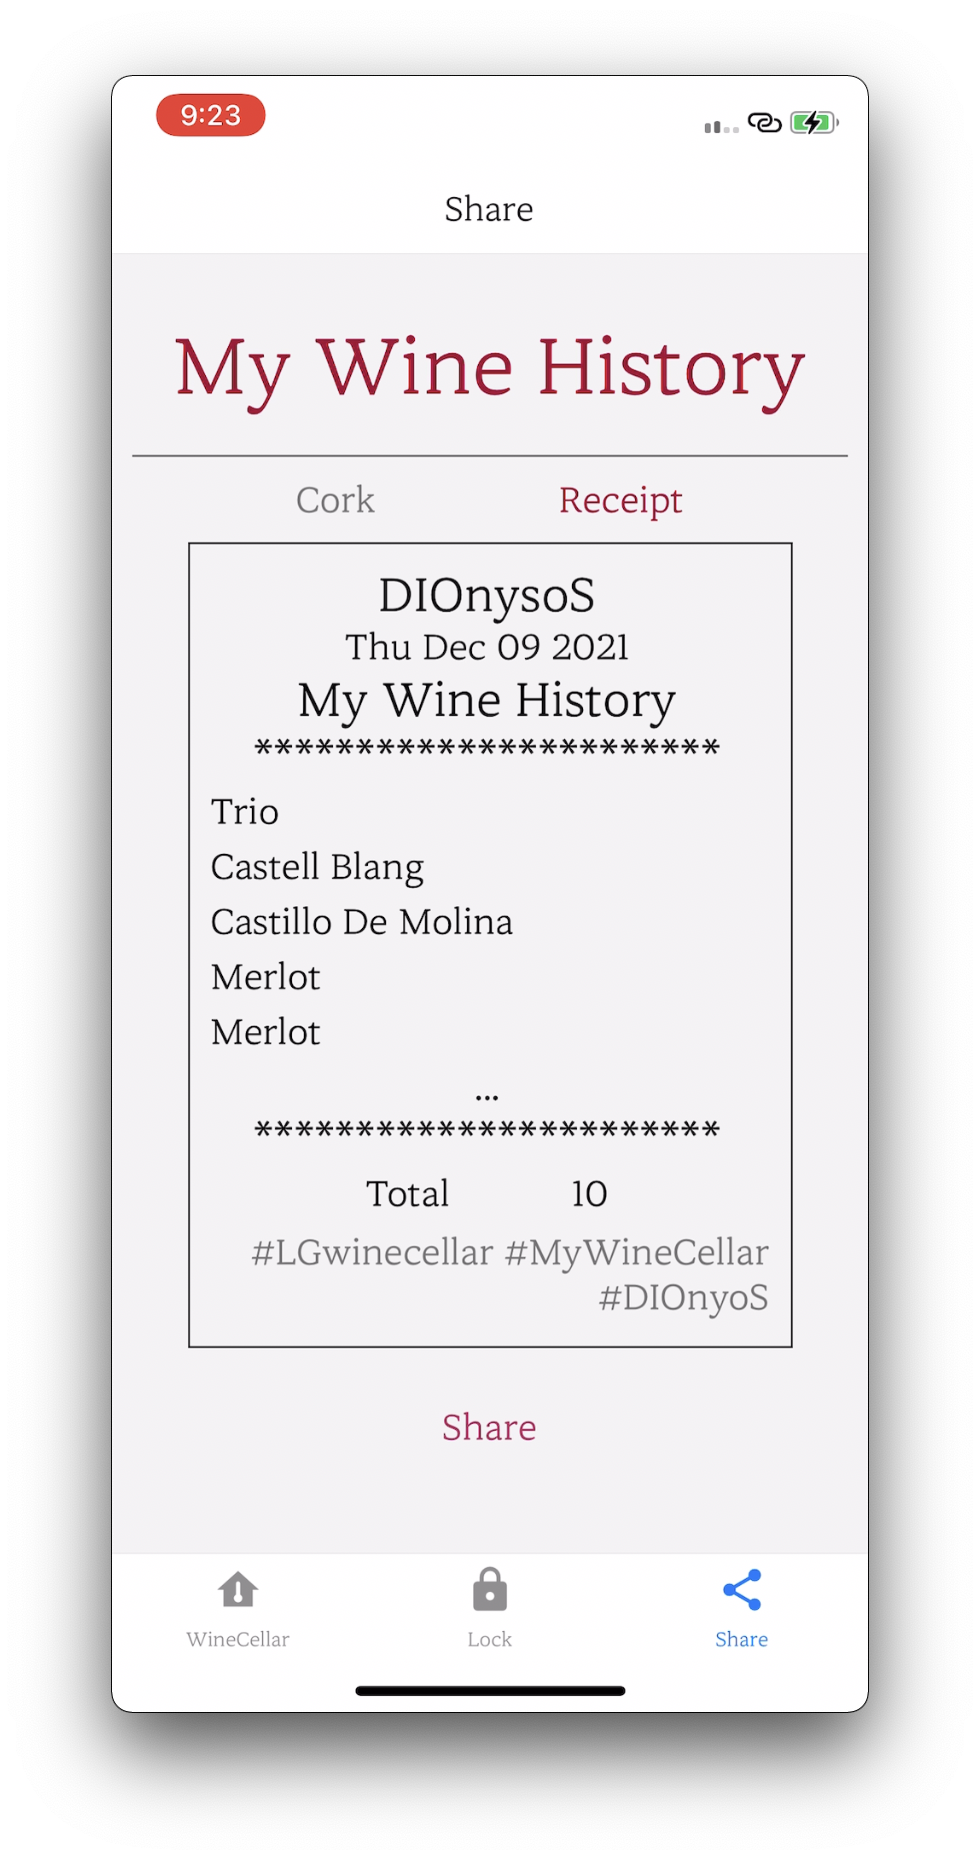
\includegraphics[width=4cm]{sharerec.png}}
                    \caption{Share Receipt}
                \end{figure}
                Wine which user has drunk until now appears as the format of receipt. Receipt is consisted of name, number and price of each wine. And total amount and price of wine will appear at the bottom of receipt.
            \end{enumerate}
            \item \textit{Make my Wine Topster [Fig.IV-B.20 $\sim$ 22]}
            \begin{enumerate}
            \begin{figure}[htb!]
                \centerline{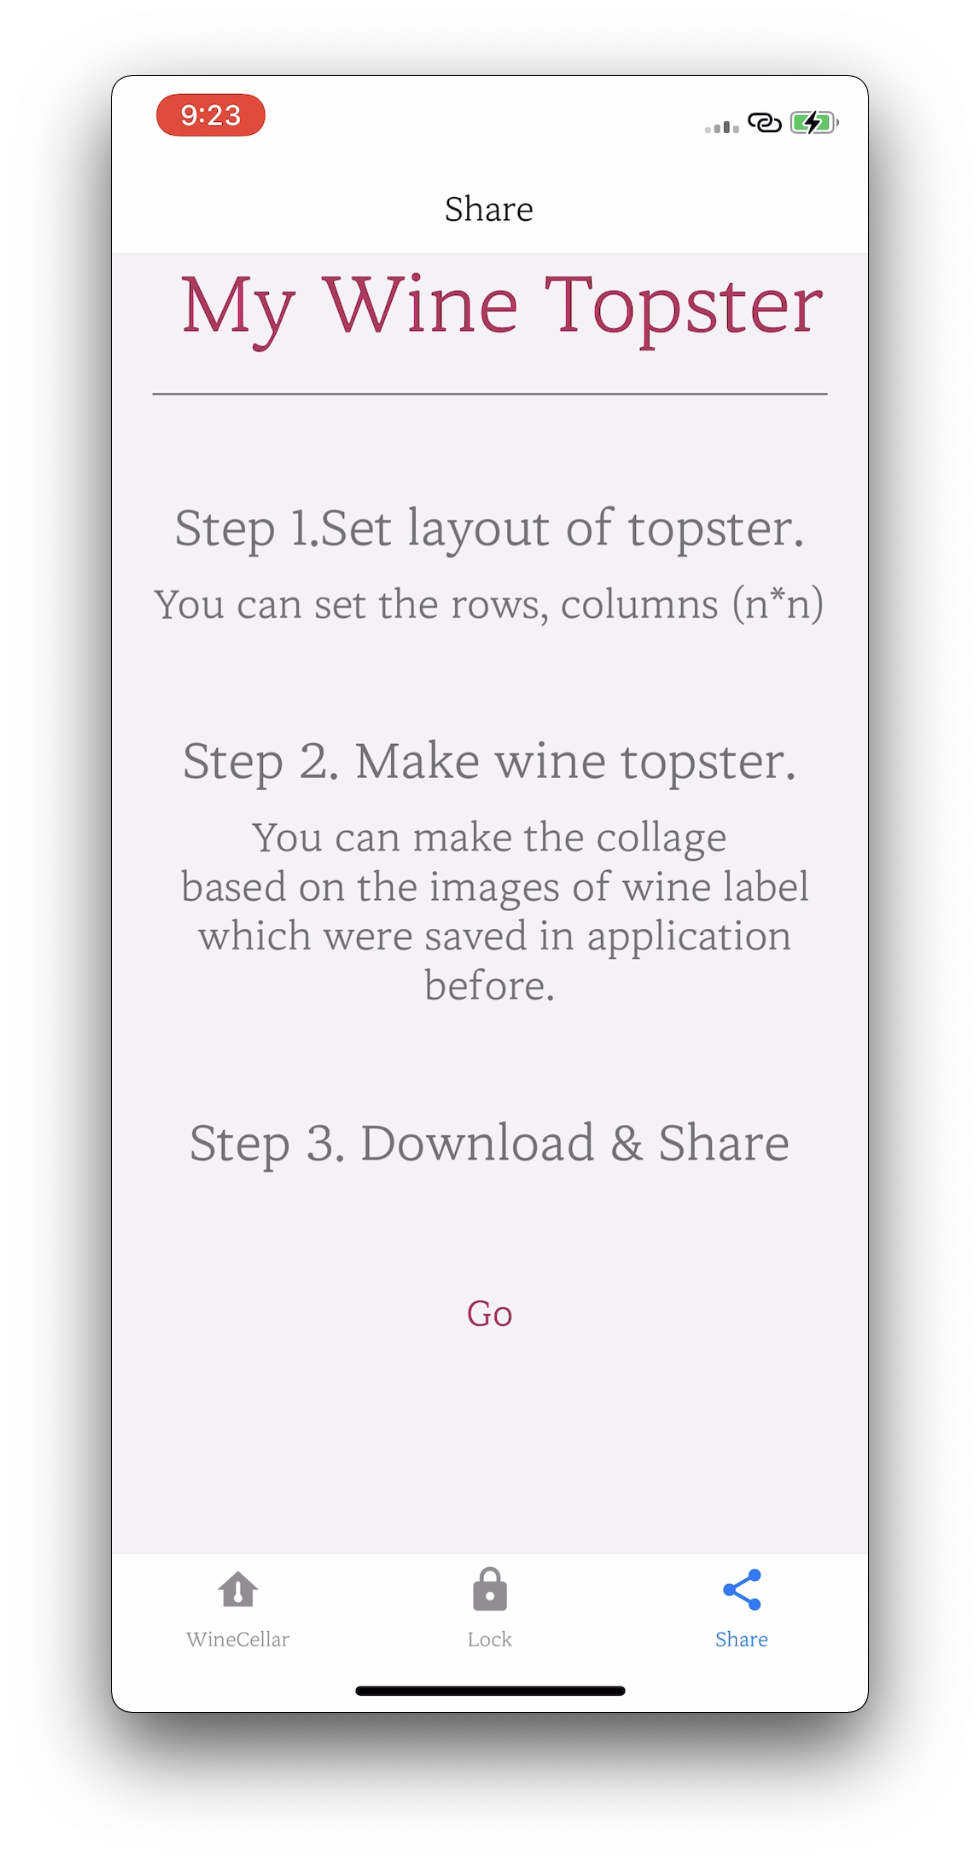
\includegraphics[width=4cm]{sharetop.png}}
                \caption{Share Topster}
            \end{figure}
                \item Description of making topster will appear. When user clicks ‘Go’ button, user can start making his own topster.
                \begin{figure}[htb!]
                    \centerline{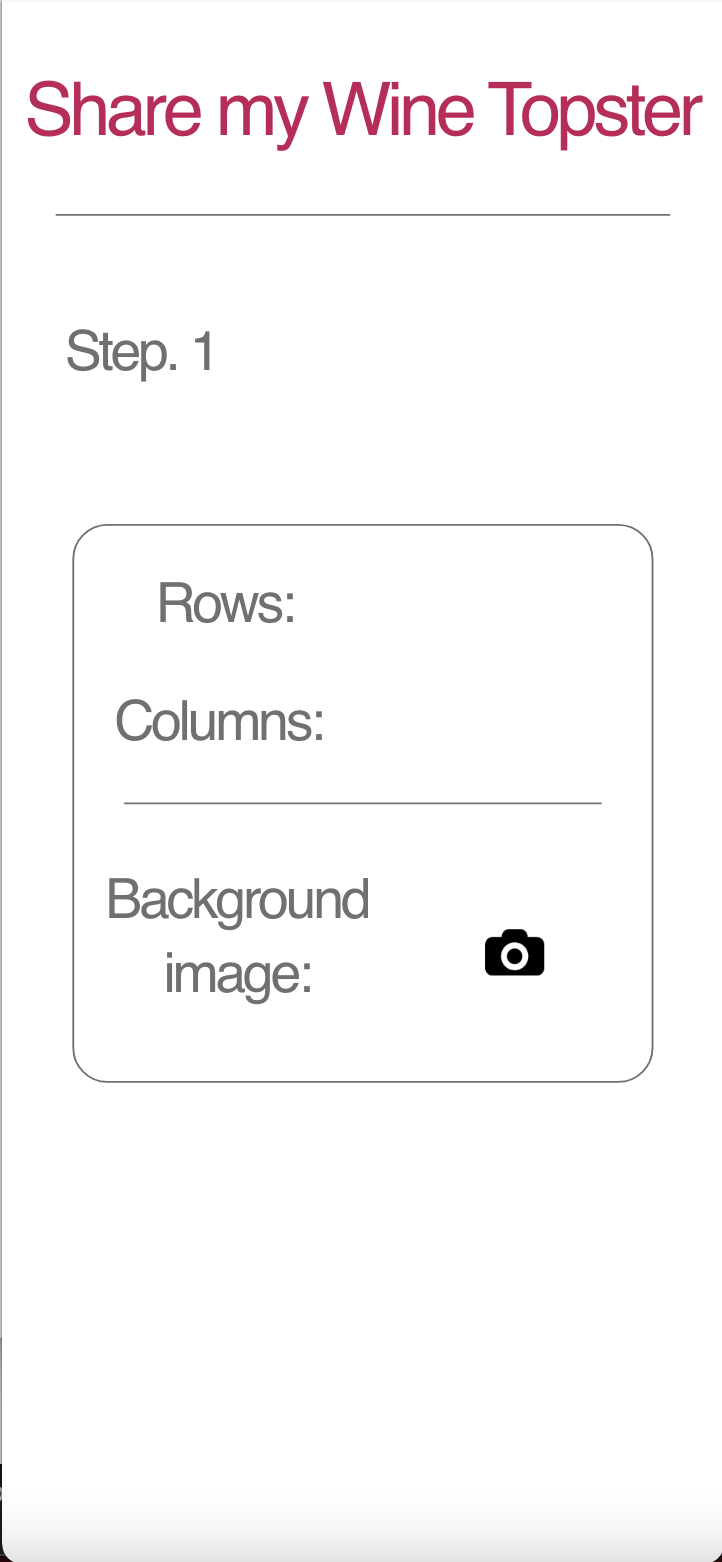
\includegraphics[width=4cm]{top1.png}}
                    \caption{Topster - I}
                \end{figure}
                \item User can set rows \& columns and background image of wine topster.
                \begin{figure}[htb!]
                    \centerline{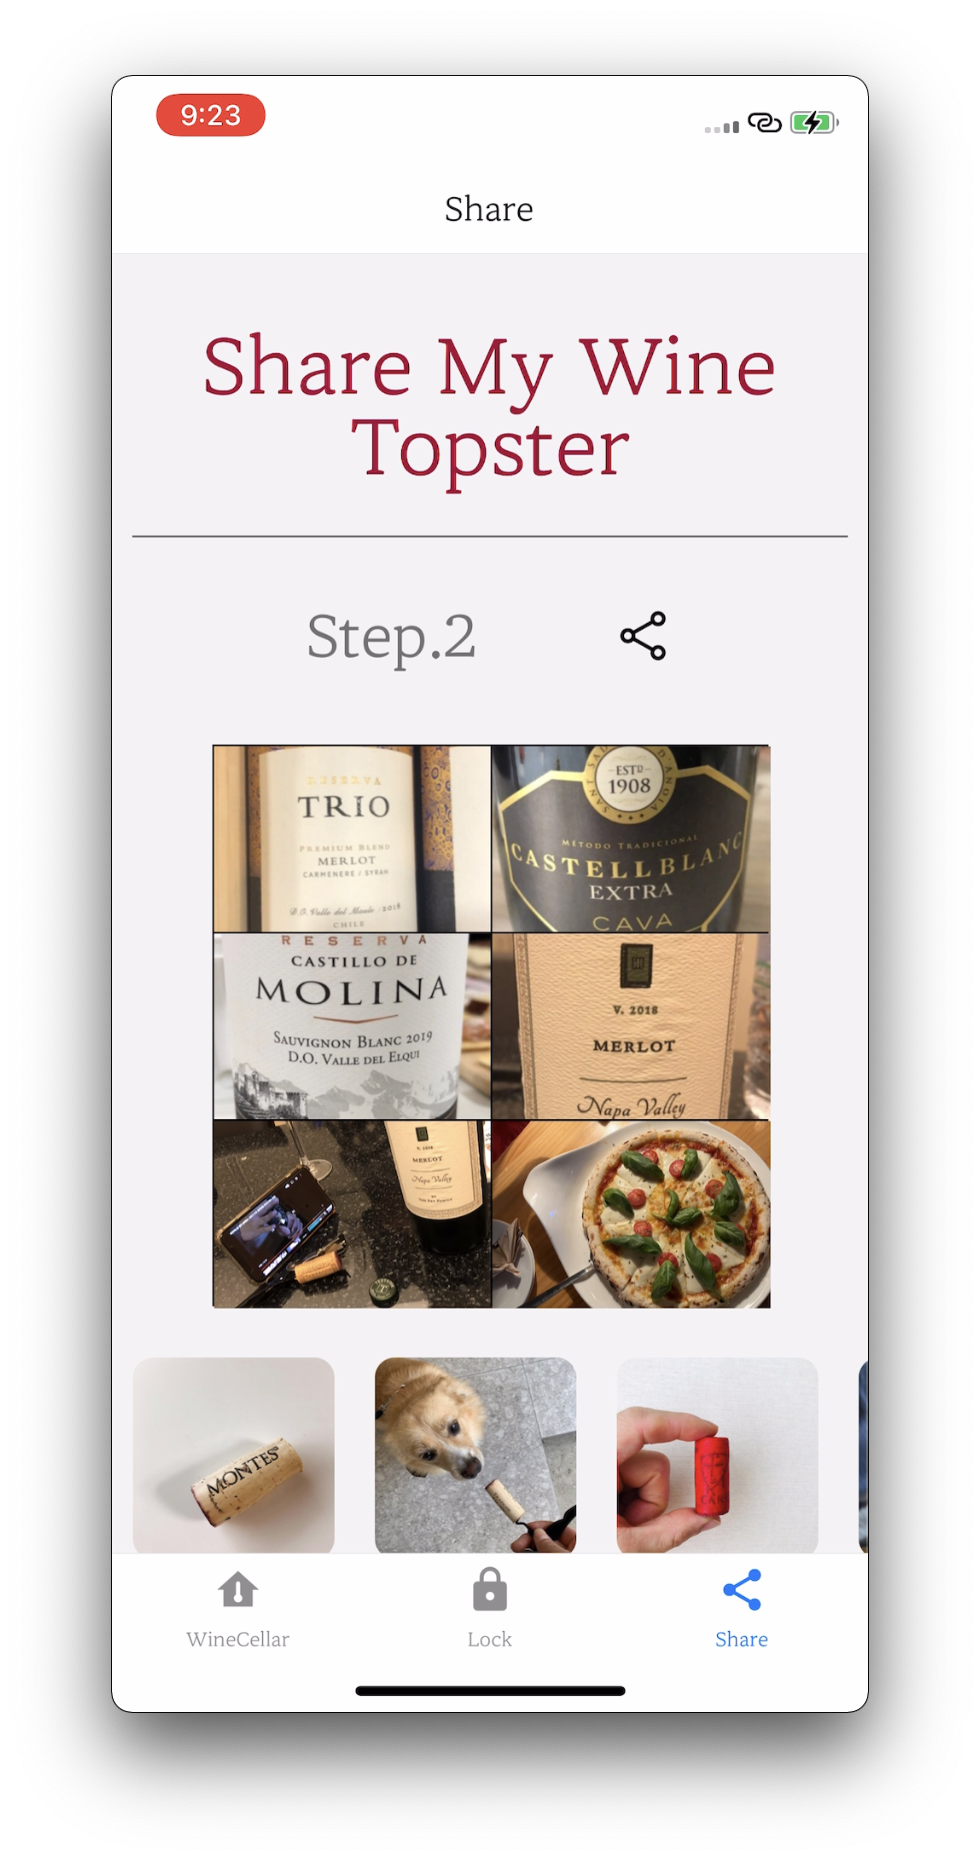
\includegraphics[width=4cm]{top2.png}}
                    \caption{Topster - II}
                \end{figure}
                \item User can make wine topster from setting. User can retrieve image of wine label from database.
            \end{enumerate}
        \end{enumerate}
    
        \item \textit{\textbf{Wine information [Fig.IV-B.23 \& 24]}}\\
        \begin{figure}[htb!]
             \centerline{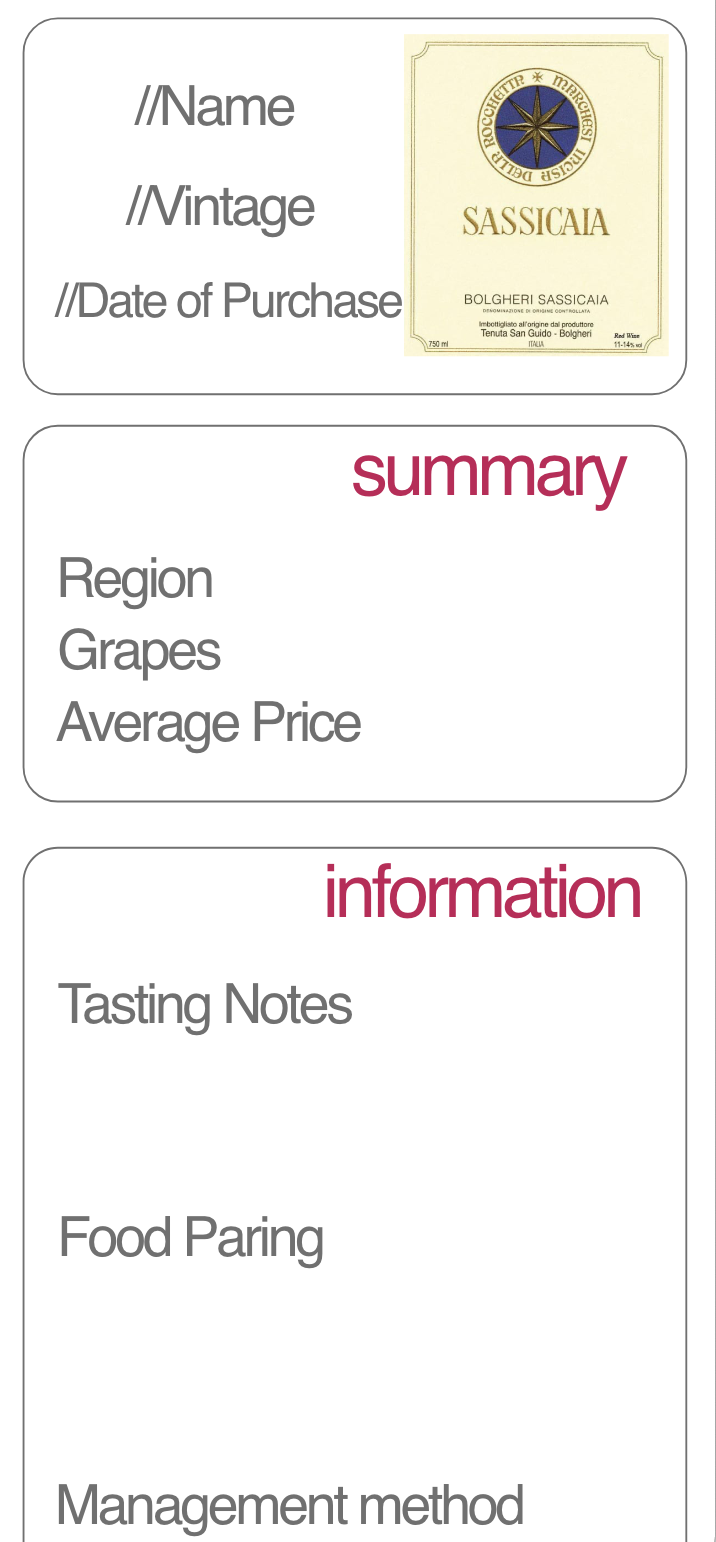
\includegraphics[width=4cm]{wineinfo.png}}
             \caption{Wine Information - I}
             \centerline{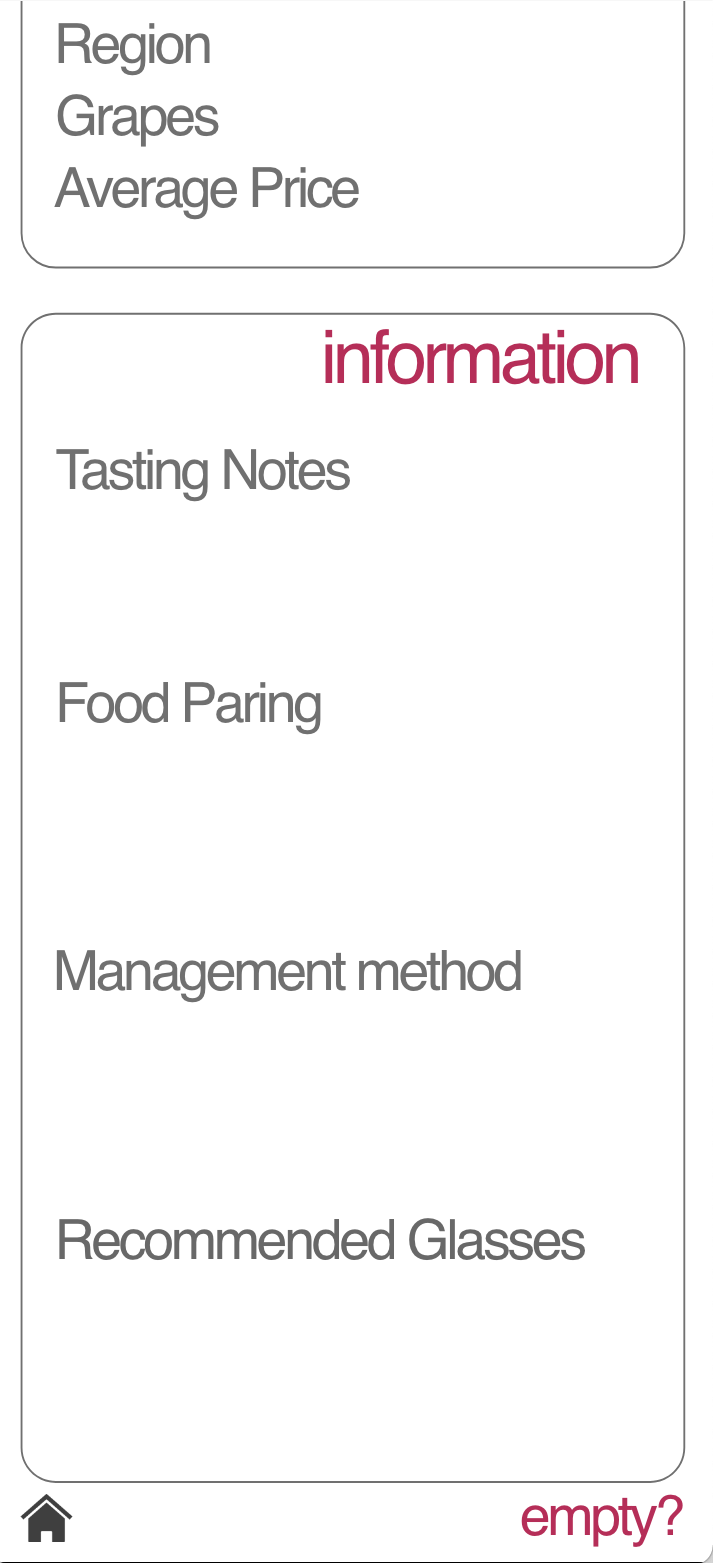
\includegraphics[width=4cm]{wineinfo2.png}}
             \caption{Wine Information - II}
         \end{figure}
        All information appears in each container tag. Photo of label, name, wine and date of purchase of wine appear in upper tag. And summary of wine, such as region, grapes and average price of wine appear in middle tag. And information of wine, such as tasting notes, food pairing, management and recommendation glasses appear in lower tag.
    \end{enumerate}
    
    \item \textit{Settings [Fig.IV-B 25]}\\
    \begin{figure}[htb!]
        \centerline{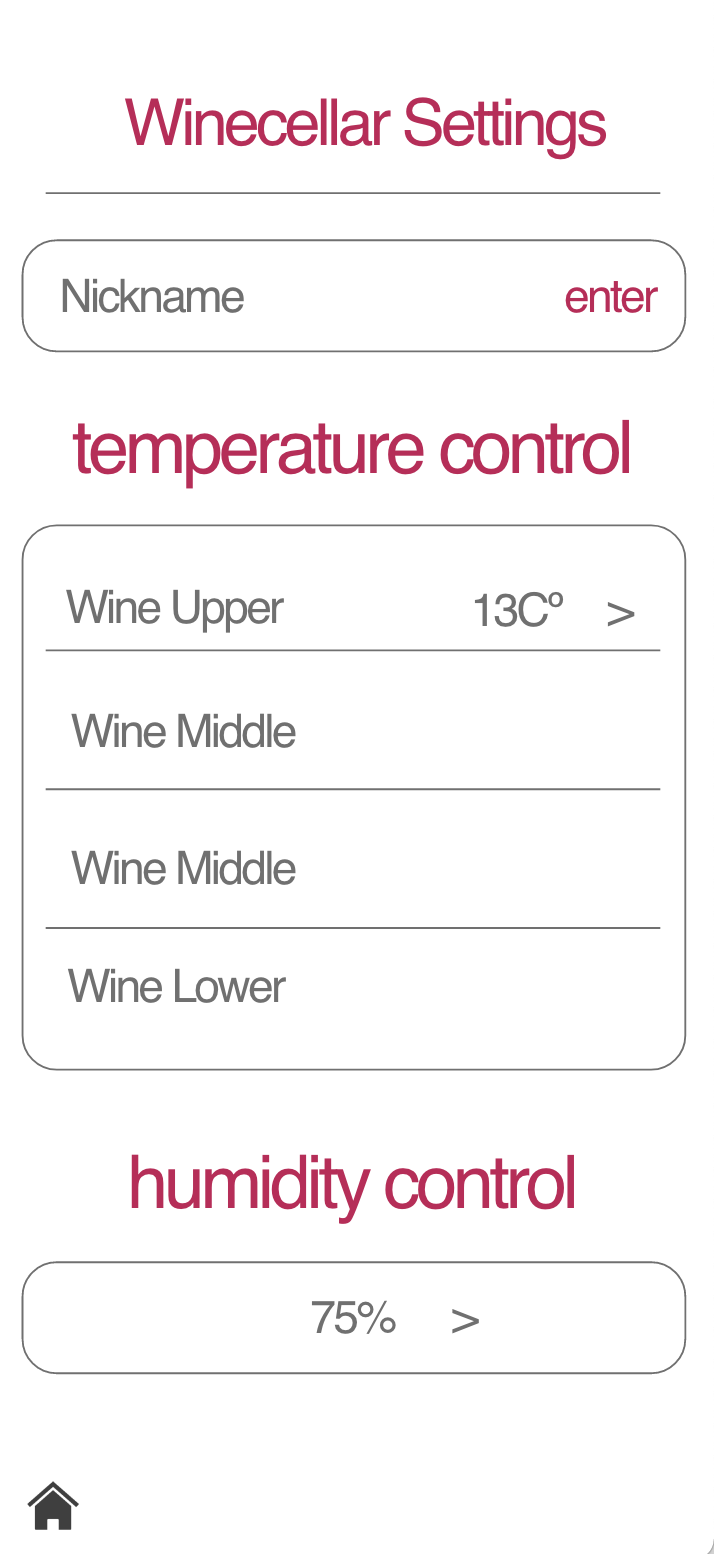
\includegraphics[width=4cm]{setting.png}}
        \caption{Settings}
    \end{figure}
    Settings icon locates next to My Wine Cellar(main page). If user pushes settings icon, user can control wine cellar.
    \begin{enumerate}
        \item \textit{Nickname}\\
        The default name of wine cellar is ‘My Wine cellar–1’. User can change it and generate own nickname. Nickname allows user who has many wine cellars to distinguish one from many wine cellar.\\
        \item \textit{Temperature control}\\
        A there is difference in appropriate temperature of wine, user can control temperature of each floor of wine cellar.
        \item \textit{Humidity control}\\
        User can control humidity of wine cellar.
        \item \textit{Image of wine label}\\
        When user clicks the image of wine label in main page, user goes to wine information page directly.
    \end{enumerate}
\end{enumerate}

\section{Architecture design and implementation}
\subsection{Overall Architecture}
\indent For our DIOnyoS application, we have several modules for the whole architecture.
First, we used React-Native for client side. It allows the application to perform several functions and implement designs. Using the application, users can register wines in winecellars and easily lock the winecellars. Also, they can share the informations of wine cellars in their social media.\\
\indent Second, we used Amazon AWS EC2, S3 for deployment, Spring framework for whole back-end section to receive and serve data to front-end section as REST API, and Node.js for running React-Native framework. Entire API server except acquiring wine image file is running on Amazon Web Services EC2 instance, and API server for acquiring wine image file is running on Amazon Web Services S3 instance. Below figure shows overall architecture of the service.These modules are interacting each other in the application. 

\centerline{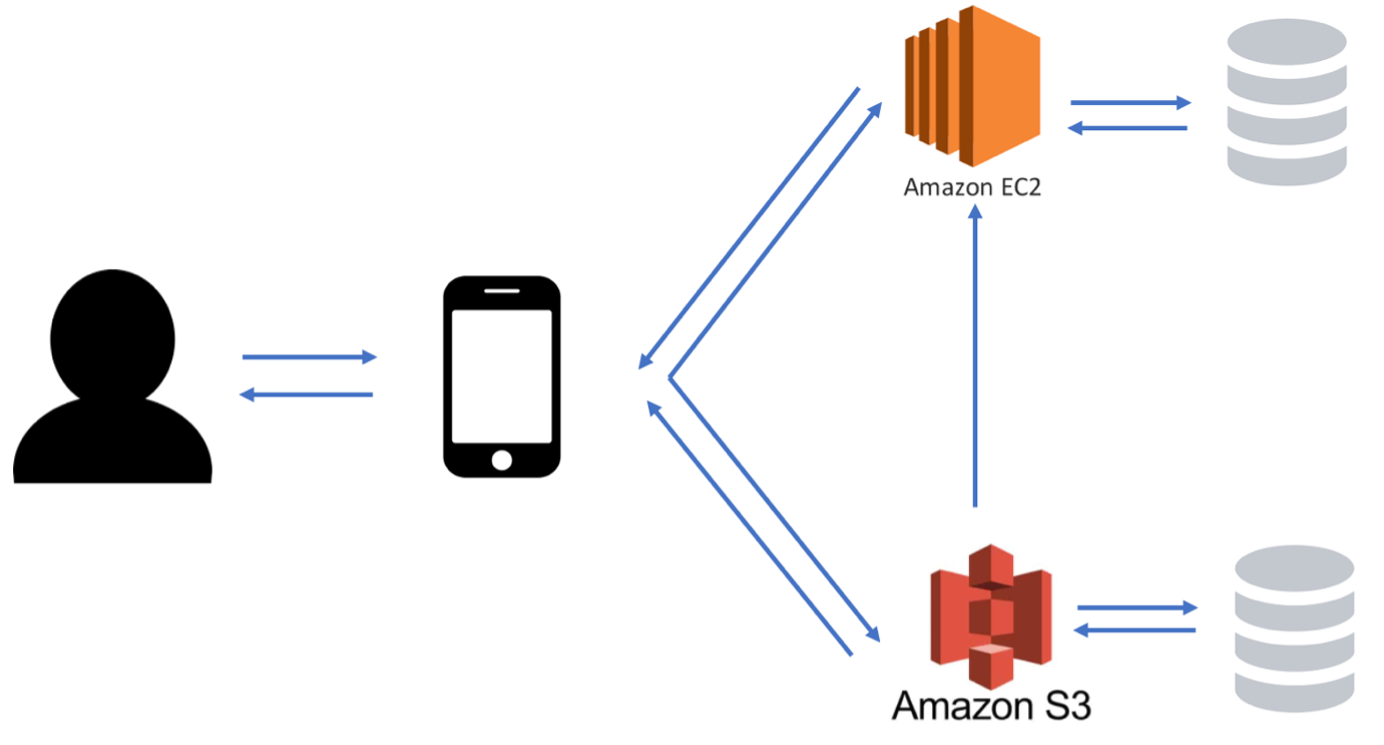
\includegraphics[width=7cm, height=4cm]{overallarch.png}}

\subsection{Database Design}
\centerline{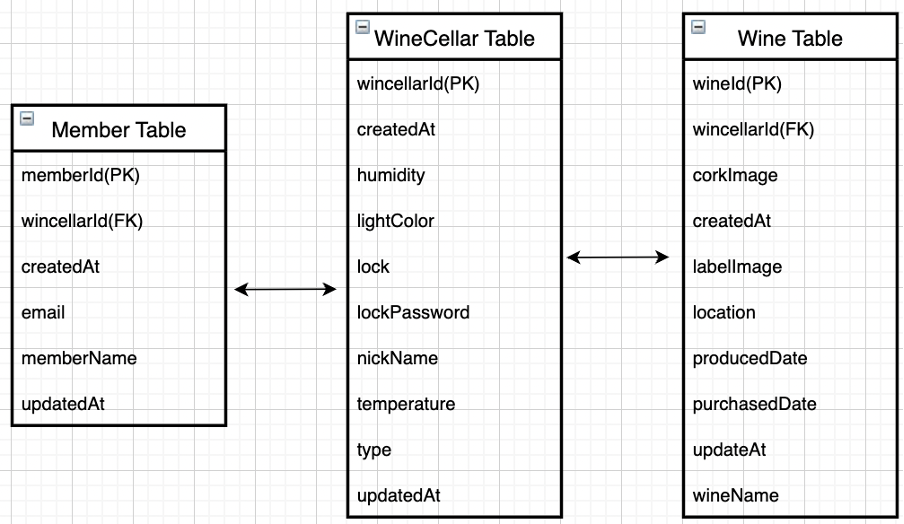
\includegraphics[width=7cm, height=4cm]{database.png}}
\begin{enumerate}
    \item \textbf{Member Table}
     \begin{enumerate}
        \item memberId(PK)\\
        identification of user
        \item createdAt\\
        date that user account created
        \item email\\
        user email
        \item memberName\\
        name of user
        \item updatedAt\\
        the date when user lastly modified their information
    \end{enumerate}
    \item \textbf{WineCellar Table}
      \begin{enumerate}
        \item     winecellarId(PK)\\
        identification of wine cellar
        \item createdAt\\
        date that wine cellar registered to database
        \item humidity\\
        the information of humidity that applied at wine cellar
        \item lightColor\\
        the information of color that currently applied to wine cellar
        \item lock\\
        status of wine cellar whether locked or not
        \item lockPassword\\
        the password to lock/unlock wine cellar
        \item nickName\\
        unique Name of wine cellar that decided by user
        \item temperature\\
        the information of temperature that currently applied to wine cellar
        \item type\\
        the type of wine cellar
        \item updatedAt\\
        the date when user lastly modified information of their wine cellar
    \end{enumerate}
    \item \textbf{Wine Table}
     \begin{enumerate}
        \item wineId(PK)\\
        identification of wine
        \item winecellarId(FK)\\
        identification of wine cellar(wine cellar that storing wine)
        \item corkImage\\
        cork image of wine took by user
        \item createAt\\
        the date that wine registered to wine cellar
        \item labelImage\\
        label image of wine
        \item location\\
        the location of wine where it stored in wine cellar
        \item producedDate\\
        the date wine produced by manufacturer
        \item purchasedDate\\
        the date wine purchased by user
        \item updateAt\\ the date when user lastly modified information of their wine
        \item wineName\\ the name of wine
    \end{enumerate}
\end{enumerate}

\subsection{Directory organization}
We are using 3 big modules which follow the overall architecture. First one is React Native, second one is Spring and the last one is Maria DB. Also, we have additional directory for LaTeX. 
    \subsubsection{Server}
    \begin{enumerate}
        \item Server/gradle/wrapper/ \\
        This directory is a collection of services that define what logic to deal with when building the application.
        \item Server/src/main/java/com/dionysos/winecellar/config \\
        This directory is a collection of files to facilitate server request processing. When user initialize the application, then WebConfig.java runs automatically to prepare user’s authentication requests.
        \item Server/src/main/java/com/dionysos/winecellar/domain/auth\\
        This directory is a collection of directories or files to handle user’s authentication requests. This directory is focused on handling authentication or confirmation of user’s token.
        \item Server/src/main/java/com/dionysos/winecellar/domain/member\\
        This directory is a collection of files to handle user request about member(user). ‘Config’ directory discern which requests are sent from client. After analyzation, ‘Service’ directory handles that request by logics that written in files in ‘Service’ directory. If SQL query requires, then files in ‘Dao’ directory create SQL query and send to database.
        \item Server/src/main/java/com/dionysos/winecellar/domain/wine\\
        This directory is a collection of files to handle user requests about wine. First, files from ‘Api’ directory receives the requests from user, and then discern which requests are sent from user. After that, files in ‘Service’ directory handles analyzed requests according to a set routine. If SQL query requires, then files in ‘Dao’ directory create SQL query and send to database. Files in ‘Dto’ create and maintain data objects.
        \item Server/src/main/java/com/dionysos/winecellar/domain/winecellar\\
        This directory is a collection of files to handle user requests about winecellar. First, files from ‘Api’ directory receives the requests from user, and then discern which requests are sent from user. After that, files in ‘Service’ directory handles analyzed requests according to a set routine. If SQL query requires, then files in ‘Dao’ directory create SQL query and send to database. Files in ‘Dto’ create and maintain data objects.
    \end{enumerate}
    \subsubsection{Client}
    \begin{enumerate}
        \item Welcome
        \begin{enumerate}
            \item Welcome\\
            This is the loading page of our application. When user clicks the image of wine glass, user can go to Kakao account-log in page. After log in, user encounters two red buttons, which is consisted of wine cellar registration and go to my winecellar. By using Welcome navigator, user can link to each page.  
            \item WelcomeNavigator 
             This is a navigation which enables transition among WelcomeScreen, LoginScreen, SelectScreen and Registration. 
        \end{enumerate}
        \item Log in Page
        \begin{enumerate}
            \item login\\
             This is the first page which user can log in. When user clicks ‘Log in with kakao’, user can log in by entering the username and password of his Kakao account. At the same time, the information of user is saved in the database.  
        \end{enumerate}
        \item Registration
        \begin{enumerate}
            \item Registration\\ 
            This is the wine cellar registration page. The input data of wine cellar registration is the serial number of wine cellar. There are two cases in the wine cellar registration process. If user enters the serial number which is in the database, the serial number and the model name of the wine cellar is shown. Else if, ‘The serial number doesn’t exit’ message alerts and it lets user to enter the serial number again. After wine cellar registration, user can connect the physical wine cellar and wine cellar in application. 
            \item RegistrationNavigator\\
            This is a navigation which enables transition between SelectScreen and Registration.
        \end{enumerate}
        \item My Wine Cellar
        \begin{enumerate}
            \item My winecellar\\
            When user clicks the setting image, user goes to WineCellarSetting page. 
            When user clicks the share image, user can share the image of wine cellar in Instagram. And ‘\#LGwinecellar, \#MyWineCellar, \#DIOnyoS’ hashtags are uploaded together in Instagram posting.
            \item WineCellarSetting\\
            There are three parts in wine cellar setting page. First part is  nickname setting page. User can freely make the nickname of wine cellar. Second part is temperature control page. User can set the temperature of physical wine cellar by our application. Third part is Humidity control page. User can set the humidity of physical wine cellar by our application.
            \item WineTab\\
            It is tab which locates in the bottom of page. By clicking wine tab, user can move to wine cellar, lock main, wine registration, wine recommendation and share navigator. 
            \item WineCellarNavigator\\
            This is a navigation which enables transition between WineCellar and WineCellarSetting.
        \end{enumerate}
        \item Lock
        \begin{enumerate}
            \item lock info\\
             This is a page for setting wine cellar password, which is for locking wine cellar. The password should be 6-digit password. When user saves the password, message which notifies that password is saved pops up.
            \item cellarlock\\
            This is a page which user can lock full floor or lock floor-by-floor. Locking full floor is done by clicking red button. And locking floor-by-floor is done by clicking each lock button. 
            \item locknavigator\\
            This is a navigation which enables transition among lock info, cellarlock and locknavigation.
        \end{enumerate}
        \item Share
        \begin{enumerate}
            \item sharehome\\
            This is a page which is consisted of three buttons. The first button is to link users to SharemyWineCellar. The second button is to link users to SharemyWineHistory. The third button is to link users to MakemyWineTopsterMain. 
            \item MyWineTopster\\
            This is a first page for explaining steps of making wine topster. When user reads all the direction and explanation, user clicks the go button, which links to MyWine.
            \item MyWineTopsterFirst\\
            This is a page for making wine topster. User can set the rows and columns of wine topster. Also, he can select background image from ‘Photos’ in his device. 
            \item MyWineTopsterNavigator\\
            This is a navigation which enables transition among sharehome, MyWineTopster and MyWineTopsterFirst.
        \end{enumerate}
    \end{enumerate}

There are two tables which show directory, file name and module name. 
\begin{table}[htbp!]
\caption{Server Directory}
    \begin{center}
        \begin{tabular}{ | m{3cm} | m{2cm}| m{1.5cm} | } 
          \hline
         \textbf{Directory}& \textbf{File name} & \textbf{Module name} \\
        \hline
          \textbf{Server/gradle/wrapper} & gradle-wrapper.jar
        gradle-wrapper.properites
         & gradle\\
          \hline
          \textbf{Server/src/main/java/com/
          dionysos/winecellar/config} & WebConfig.java
         & Spring \\ 
          \hline
          \textbf{Server/src/main/java/com/
          dionysos/winecellar/domain/auth} & Auth-
          Controller.java
        AuthResponseDto.java
        LoginDto.java
        
         & Spring\\
          \hline
         \textbf{Server/src/main/java/com/
         dionysos/winecellar/domain/member/}& LoginMember-
         Id.java
        MemberRepository.java
        Member.java
        MemberService.java
        …
        
        & Spring,
        Lombok
         \\
        \hline
          \textbf{/Server/src/main/java/com/
          dionysos/winecellar/domain/wine/} & Wine
          Controller.java
        WineRepository.java
        WineService.java
        Wine.java
        
         & RSpring,
        Lombok
         \\
          \hline
          \textbf{Server/src/main/java/com/
          dionysos/winecellar/domain/winecellar/} & Winecellar-
          Controller.java
        WinecellarRepository.java
        Winecellar.java
        WineDto.java
        …
        
         & Spring,
        Lombok
        \\
          \hline
        \end{tabular}
    \end{center}
\end{table}

\begin{table}[htbp!]
    \caption{Client Directory}
    \begin{center}
        \begin{tabular}{ | m{3cm} | m{2cm}| m{1.5cm} | } 
          \hline
         \textbf{Directory}& \textbf{File name} & \textbf{Module name} \\
        \hline
          \textbf{/src/screens/welcome} & Welcome.js
        WelcomeNavigator.js
         & React Native \\
          \hline
          \textbf{/src/screens/welcome/login} & Login.js
        SocialWebview.js
        SocialWebviewModal.js
         & React Native Axios  \\ 
          \hline
          \textbf{/src/screens/winecellar} & WineCellar.js
        WineCellarNavigator.js
        WineCellarSetting.js
        WineTab.js
         & React Native\\
          \hline
         \textbf{/src/screens/registration}& Registration.js
        RegistrationNavigator.js
        & React Native \\
        \hline
          \textbf{/src/screens/share} & ShareHome.js
        ShareNavigator.js
        ShareWineCellar.js
        InstagramShare.js
        MyWineTopsterNavigator.js
        MyWineTopsterMain.js
        MyWineTopsterFirst.js
        MyWineTopsterSecond.js
        MyWineTopsterThird.js
         & React Native \\
          \hline
          \textbf{/src/screens/lock} & LockMain.js
        LockNavigator.js
        LockInfo.js
        CellarLock.js  LockGate.js
         & React Native\\
          \hline
            \textbf{/src/screens/share} & ShareHome.js
        ShareNavigator.js
        ShareWineCellar.js
        InstagramShare.js
        MyWineTopsterNavigator.js
        MyWineTopsterMain.js
        MyWineTopsterFirst.js
        MyWineTopsterSecond.js
        MyWineTopsterThird.js
         & React Native \\
          \hline
          \textbf{/src/context} & WinecellarContext.js
         & React \\ 
          \hline
          \textbf{/src/api} & winecellarApi.js
         & React Native\\
          \hline
        \end{tabular}
    \end{center}
\end{table}

\subsection{Module 1}
\begin{enumerate}
    \item React Native\\
    We use React Native to develop a wine cellar management application for the Apple device, such as IPhone and IPad. It acts as a connection between the user and the server. It also receives the user’s input value, passes it to the backend and shows the stored value of database. 
    \item Axios\\
    We use Axios module for handling request and response from REST API, such as acquiring information of one's wine cellar and sending the password of wine cellar to enable/disable cellar lock function. Axios is Promise based HTTP client for the browser and Node.js. It is used to request data from API server.
    \item React\\
    React Native is based on React. 
    React is a free and open-source front-end JavaScript library for building user interfaces based on UI components. 
\end{enumerate}
    
\section{Use cases}
\subsection{Frontend UI}
\begin{enumerate}
    \item WineCellar Main Page
    \begin{enumerate}
        \item My WineCellar Page\\
        This is a main page of DIOnyoS when the user succeeds in logging in and registers a wine seller. My WineCellar Page shows statement of the physical LG winecellar. Depending on the winecellar model, the number of floors varies. The page shows the images of wine label saved in the application. The title container has two icons, which are Setting and Share. By pressing Setting icon, user goes to the My WineCellar setting page. And By pressing Share icon, user can share the image of winecellar in the Instagram with the hashtag '\#LGwinecellar \#MyWineCellar \#DIOnyoS'.
        \begin{enumerate}
            \item Wine Register
            \item Wine Information (Detail)
            
            - Empty\\
            % + Wine Information 안에 Empty 추가
        \end{enumerate}
        \item WineCellar Tab Bar (Bottom-Tab)\\
        At the bottom of the page, there are tab navigation bar which is consisted of three icons: WineCellar, Lock and Share. 
        \begin{enumerate}
            \item WineCellar\\
            It works like 'Home' button in the DIOnysoS. Whenever the user presses this button, the user goes to the 'My WineCeller Page' which is the main page of DIOnysoS.
            \item Lock\\
            Lock page is the one of main functions of the application. Users can use this function to prevent their wine celler from being opened their doors without passwords.
            \item Share\\
            Users can share the wine they have drunk whenever they want. Users can share photos of corks or labels of finished wine or only share wine history page without photos.
        \end{enumerate}
    \end{enumerate}
    \item Lock Page
    \begin{enumerate}
        \item Password: Setting\\
        % 사진들 일단 주석
        \begin{comment}
            \begin{figure}[ht]
                \centering
                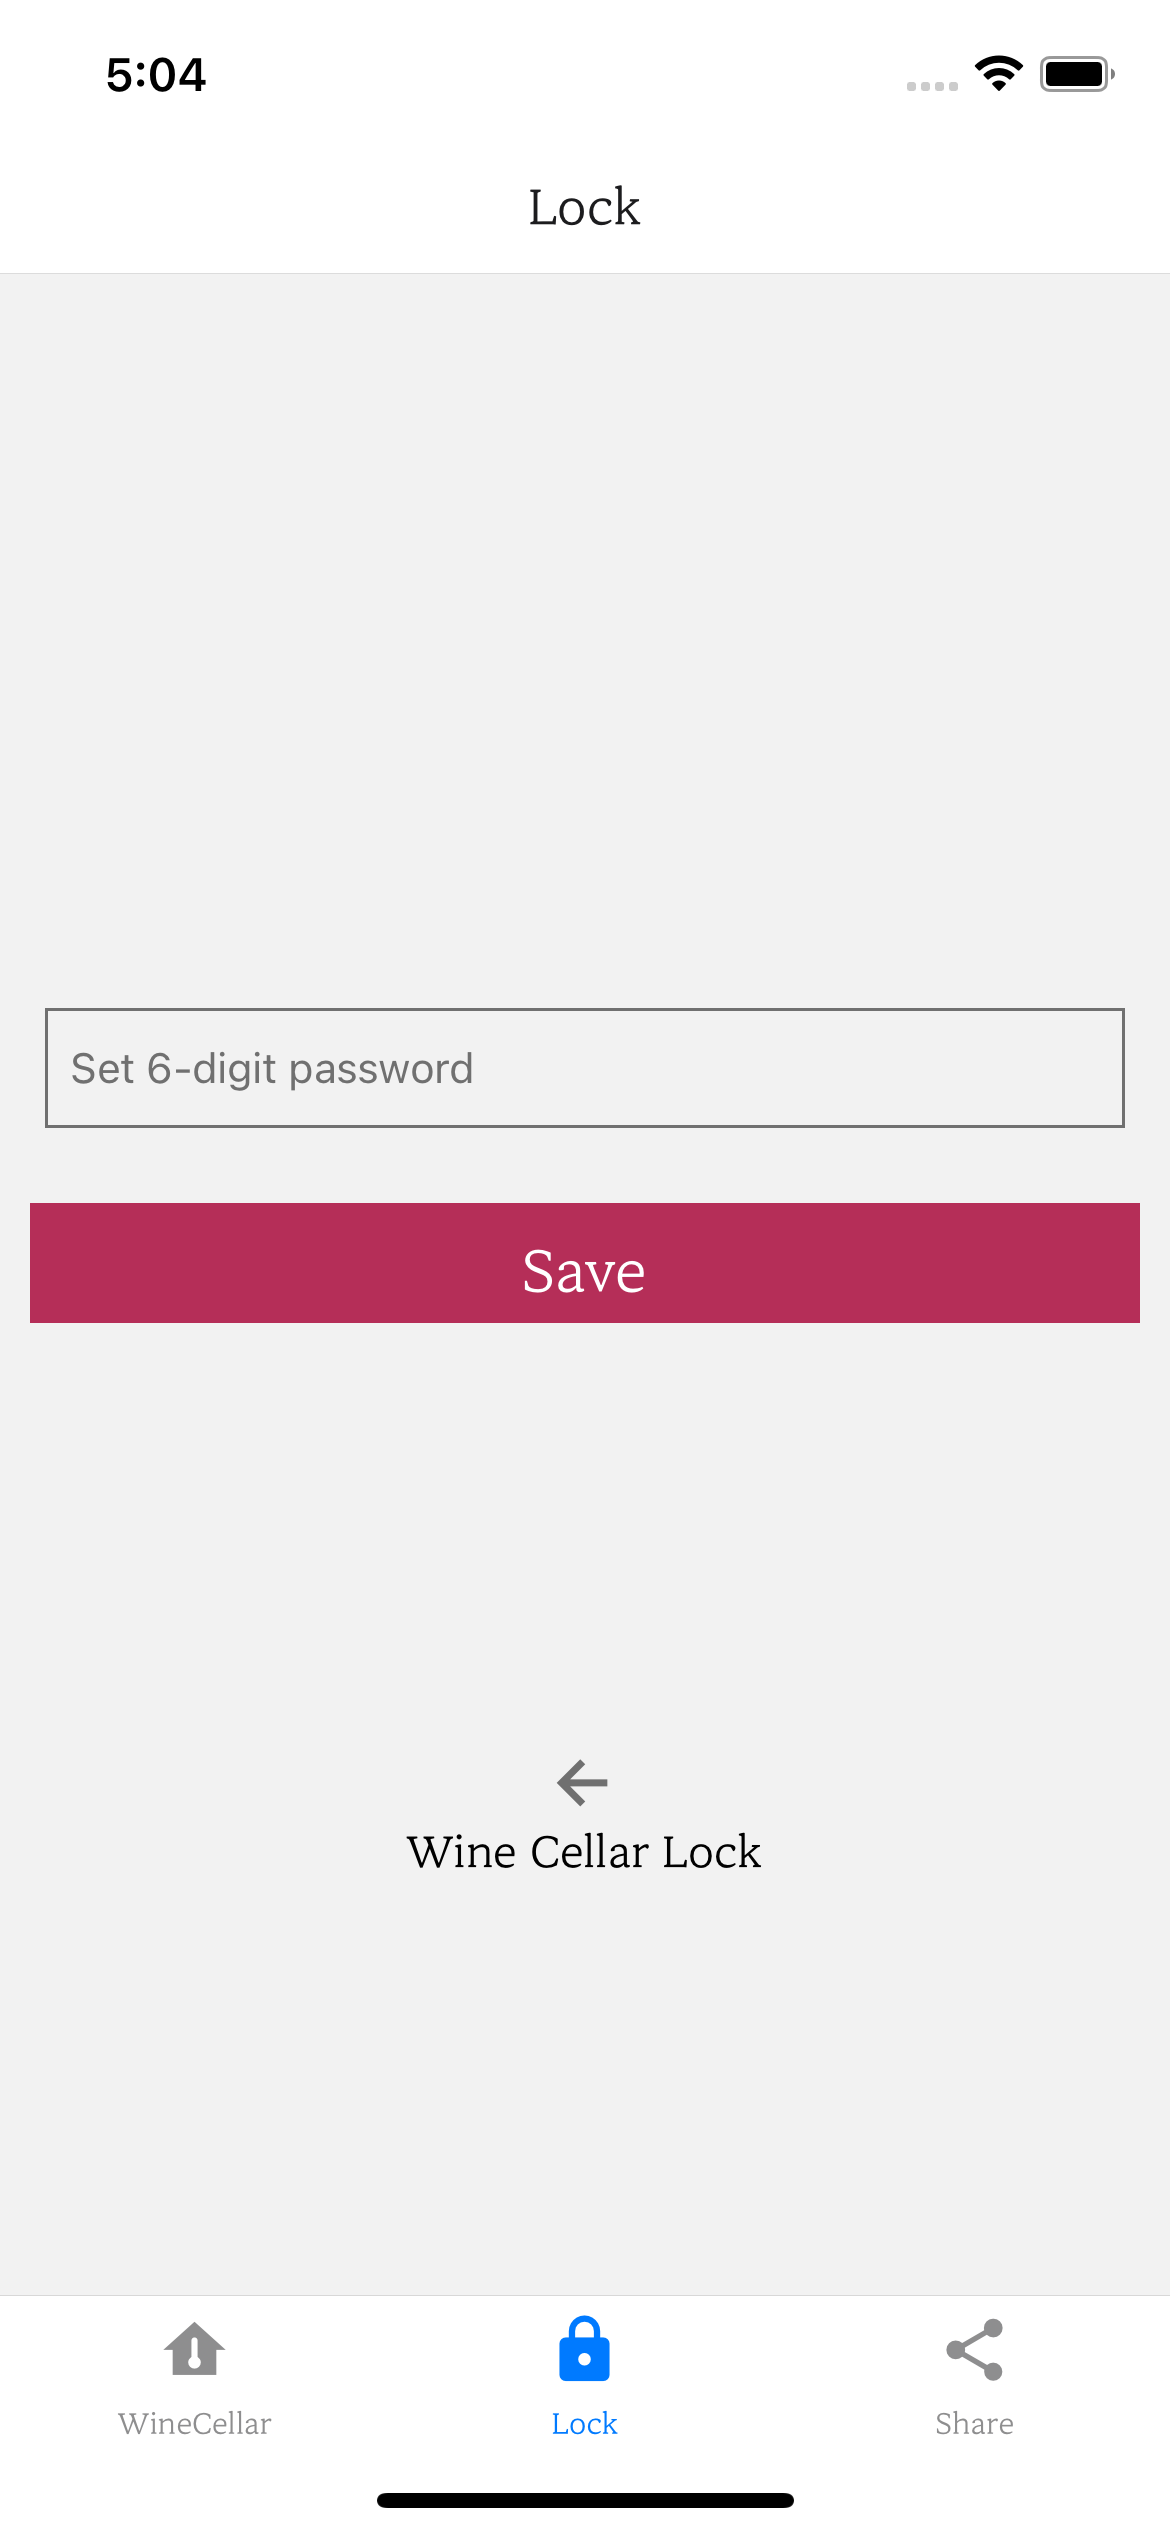
\includegraphics[width=5cm]{2. WineCellarPasswdSetting.png}
                \caption{Password Setting}
            \end{figure}
            \begin{figure}[ht]
                \centering
                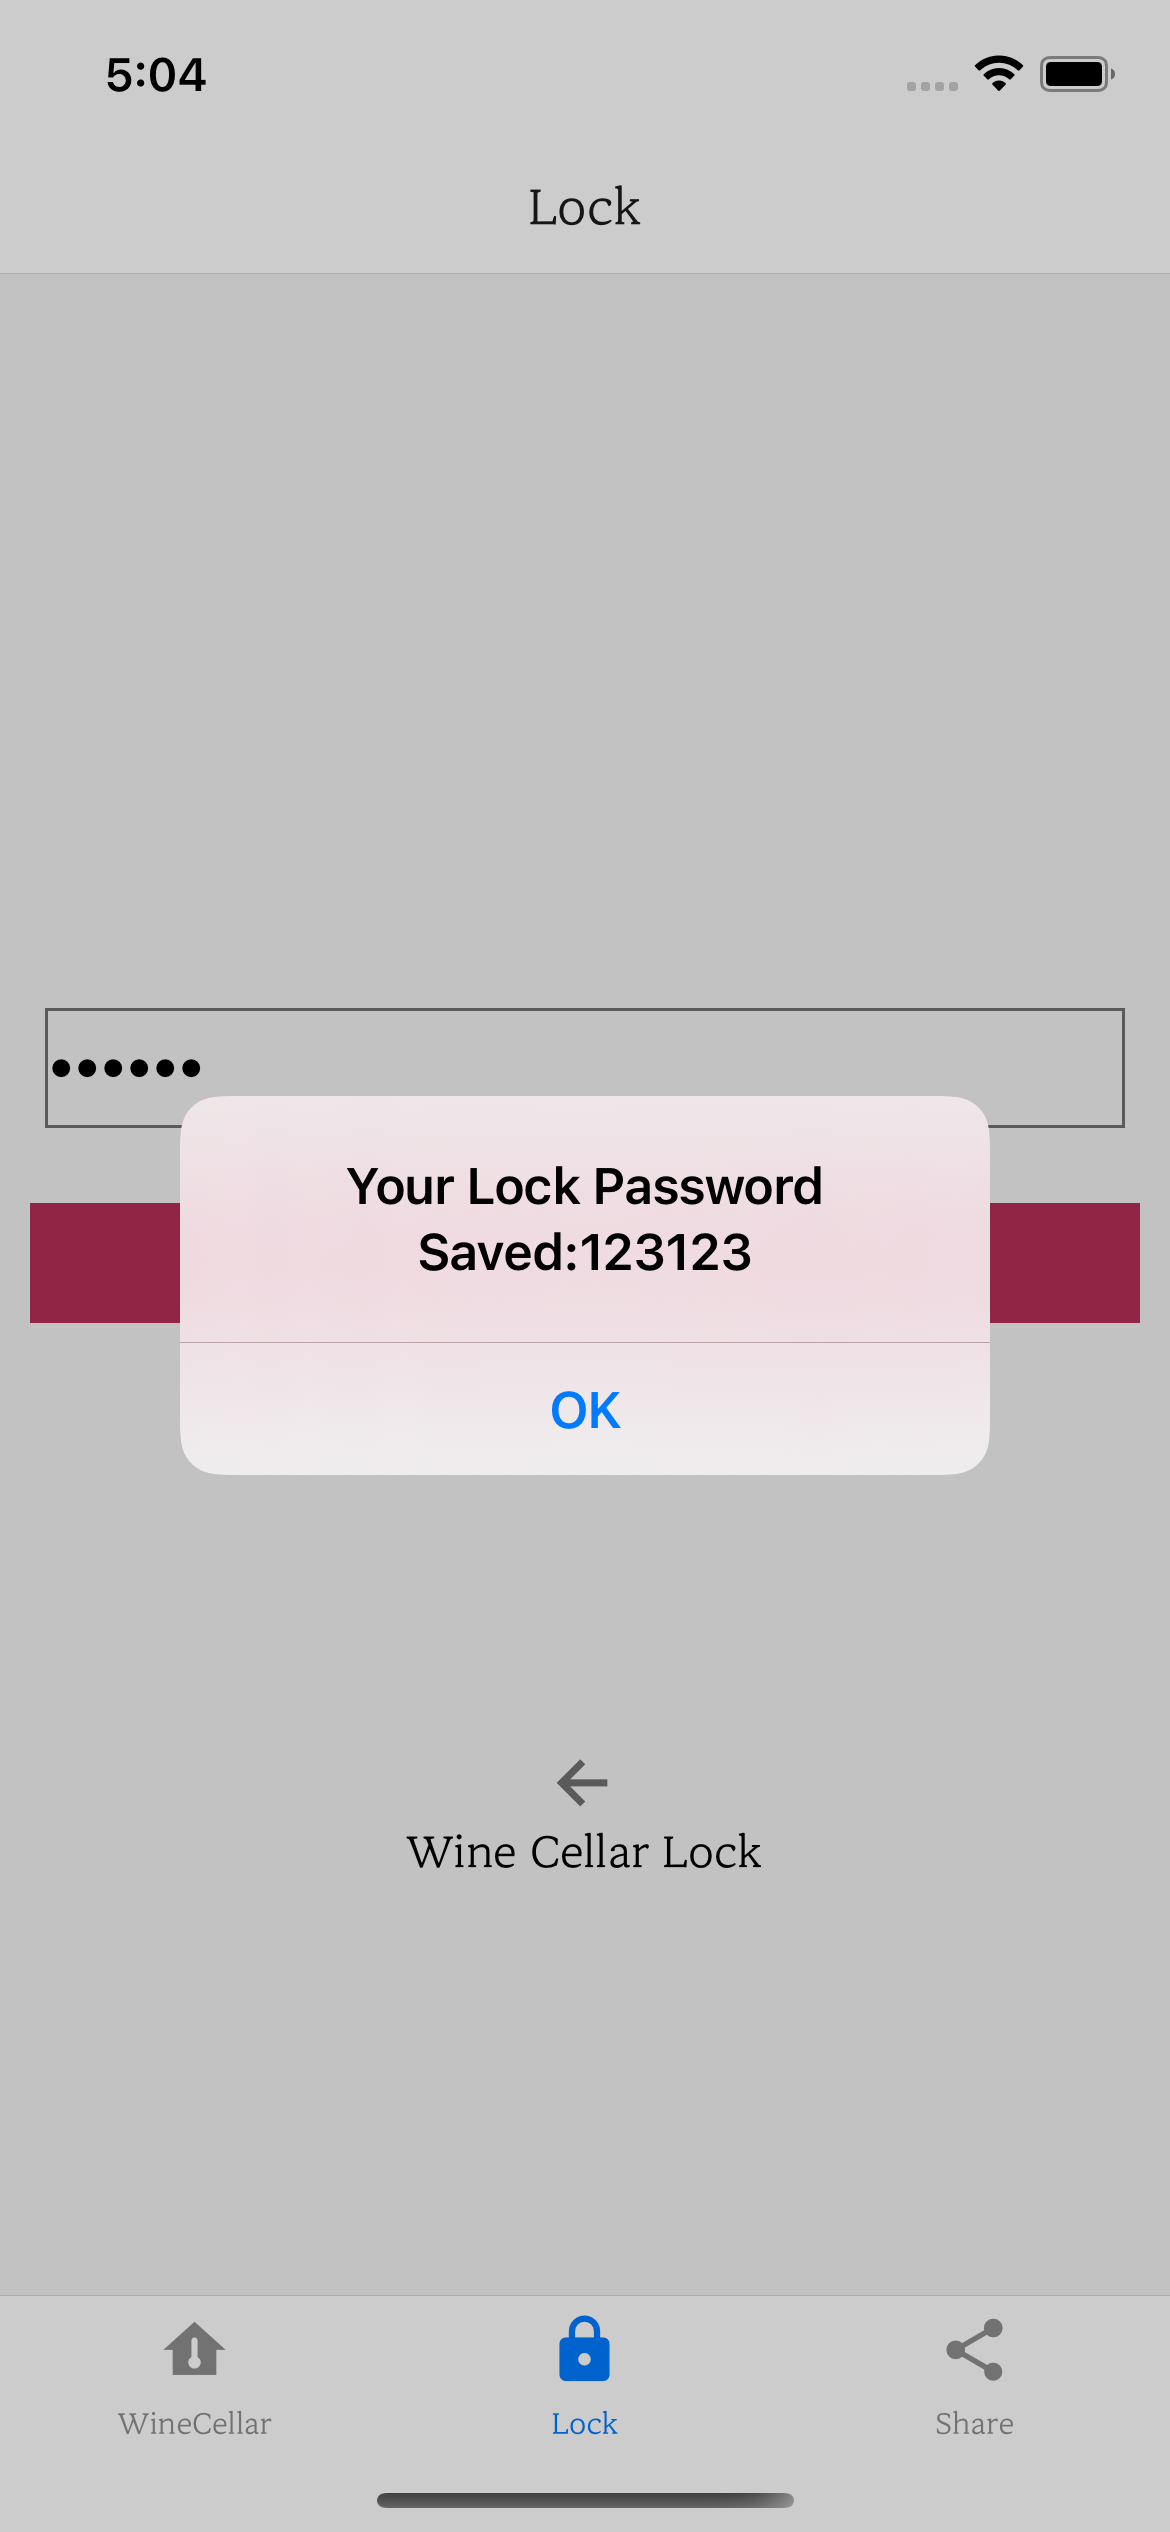
\includegraphics[width=5cm]{3. Winecellar AfterSetPasswd.png}
                \caption{Password Setting}
            \end{figure}
            \begin{figure}[ht]
                \centering
                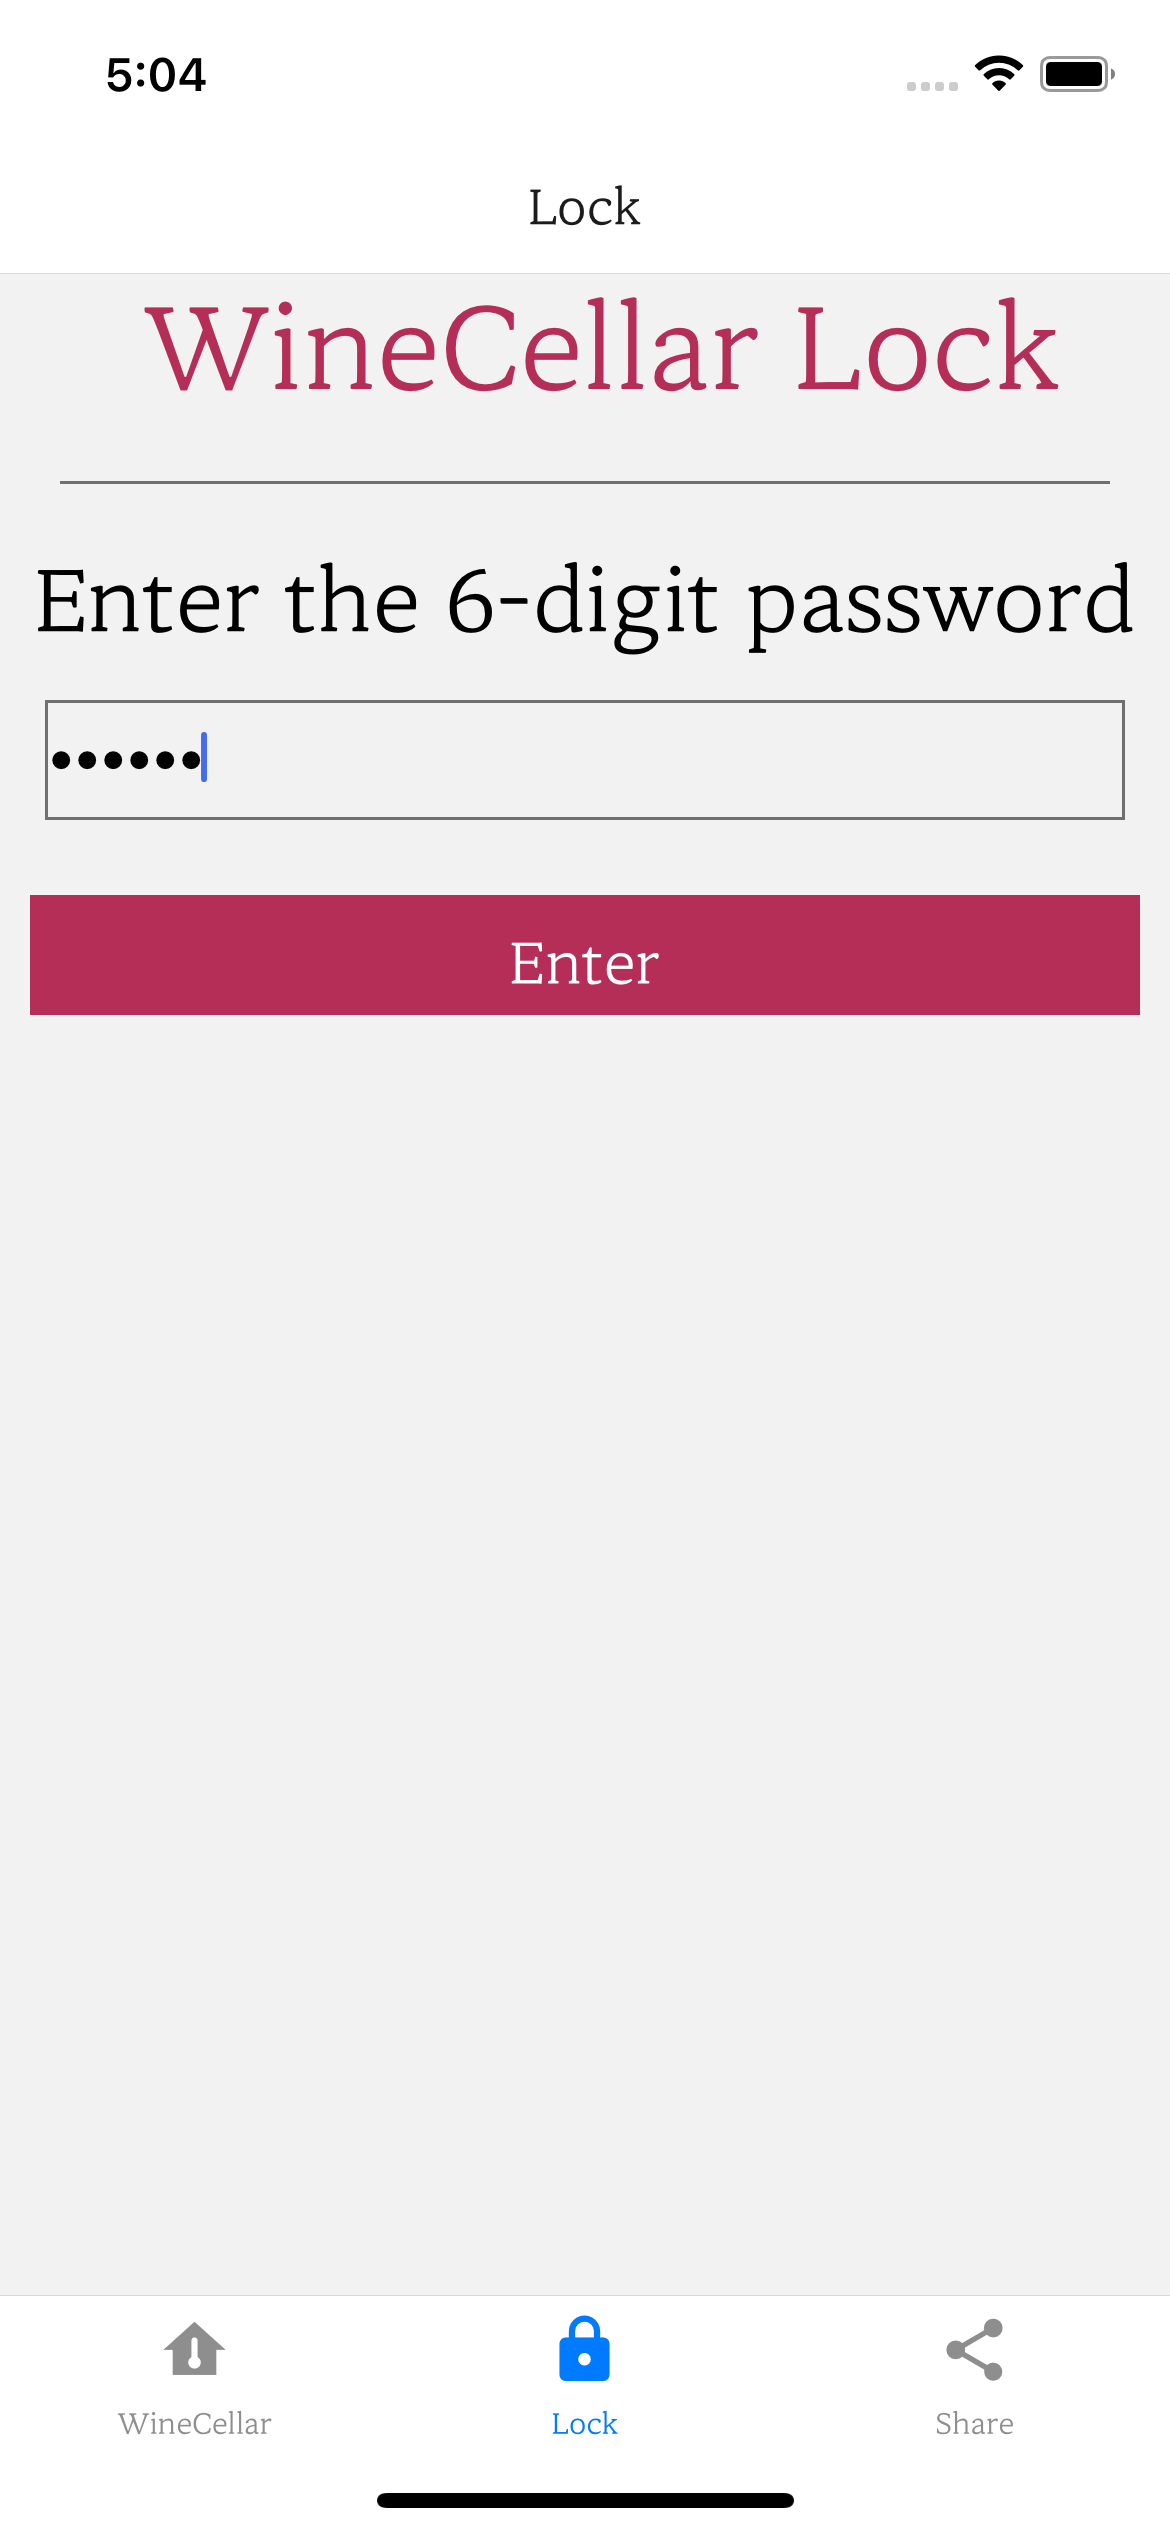
\includegraphics[width=5cm]{4. Passwd Confirmation.png}
                \caption{Password Setting}
            \end{figure}
            \begin{figure}[ht]
                \centering
                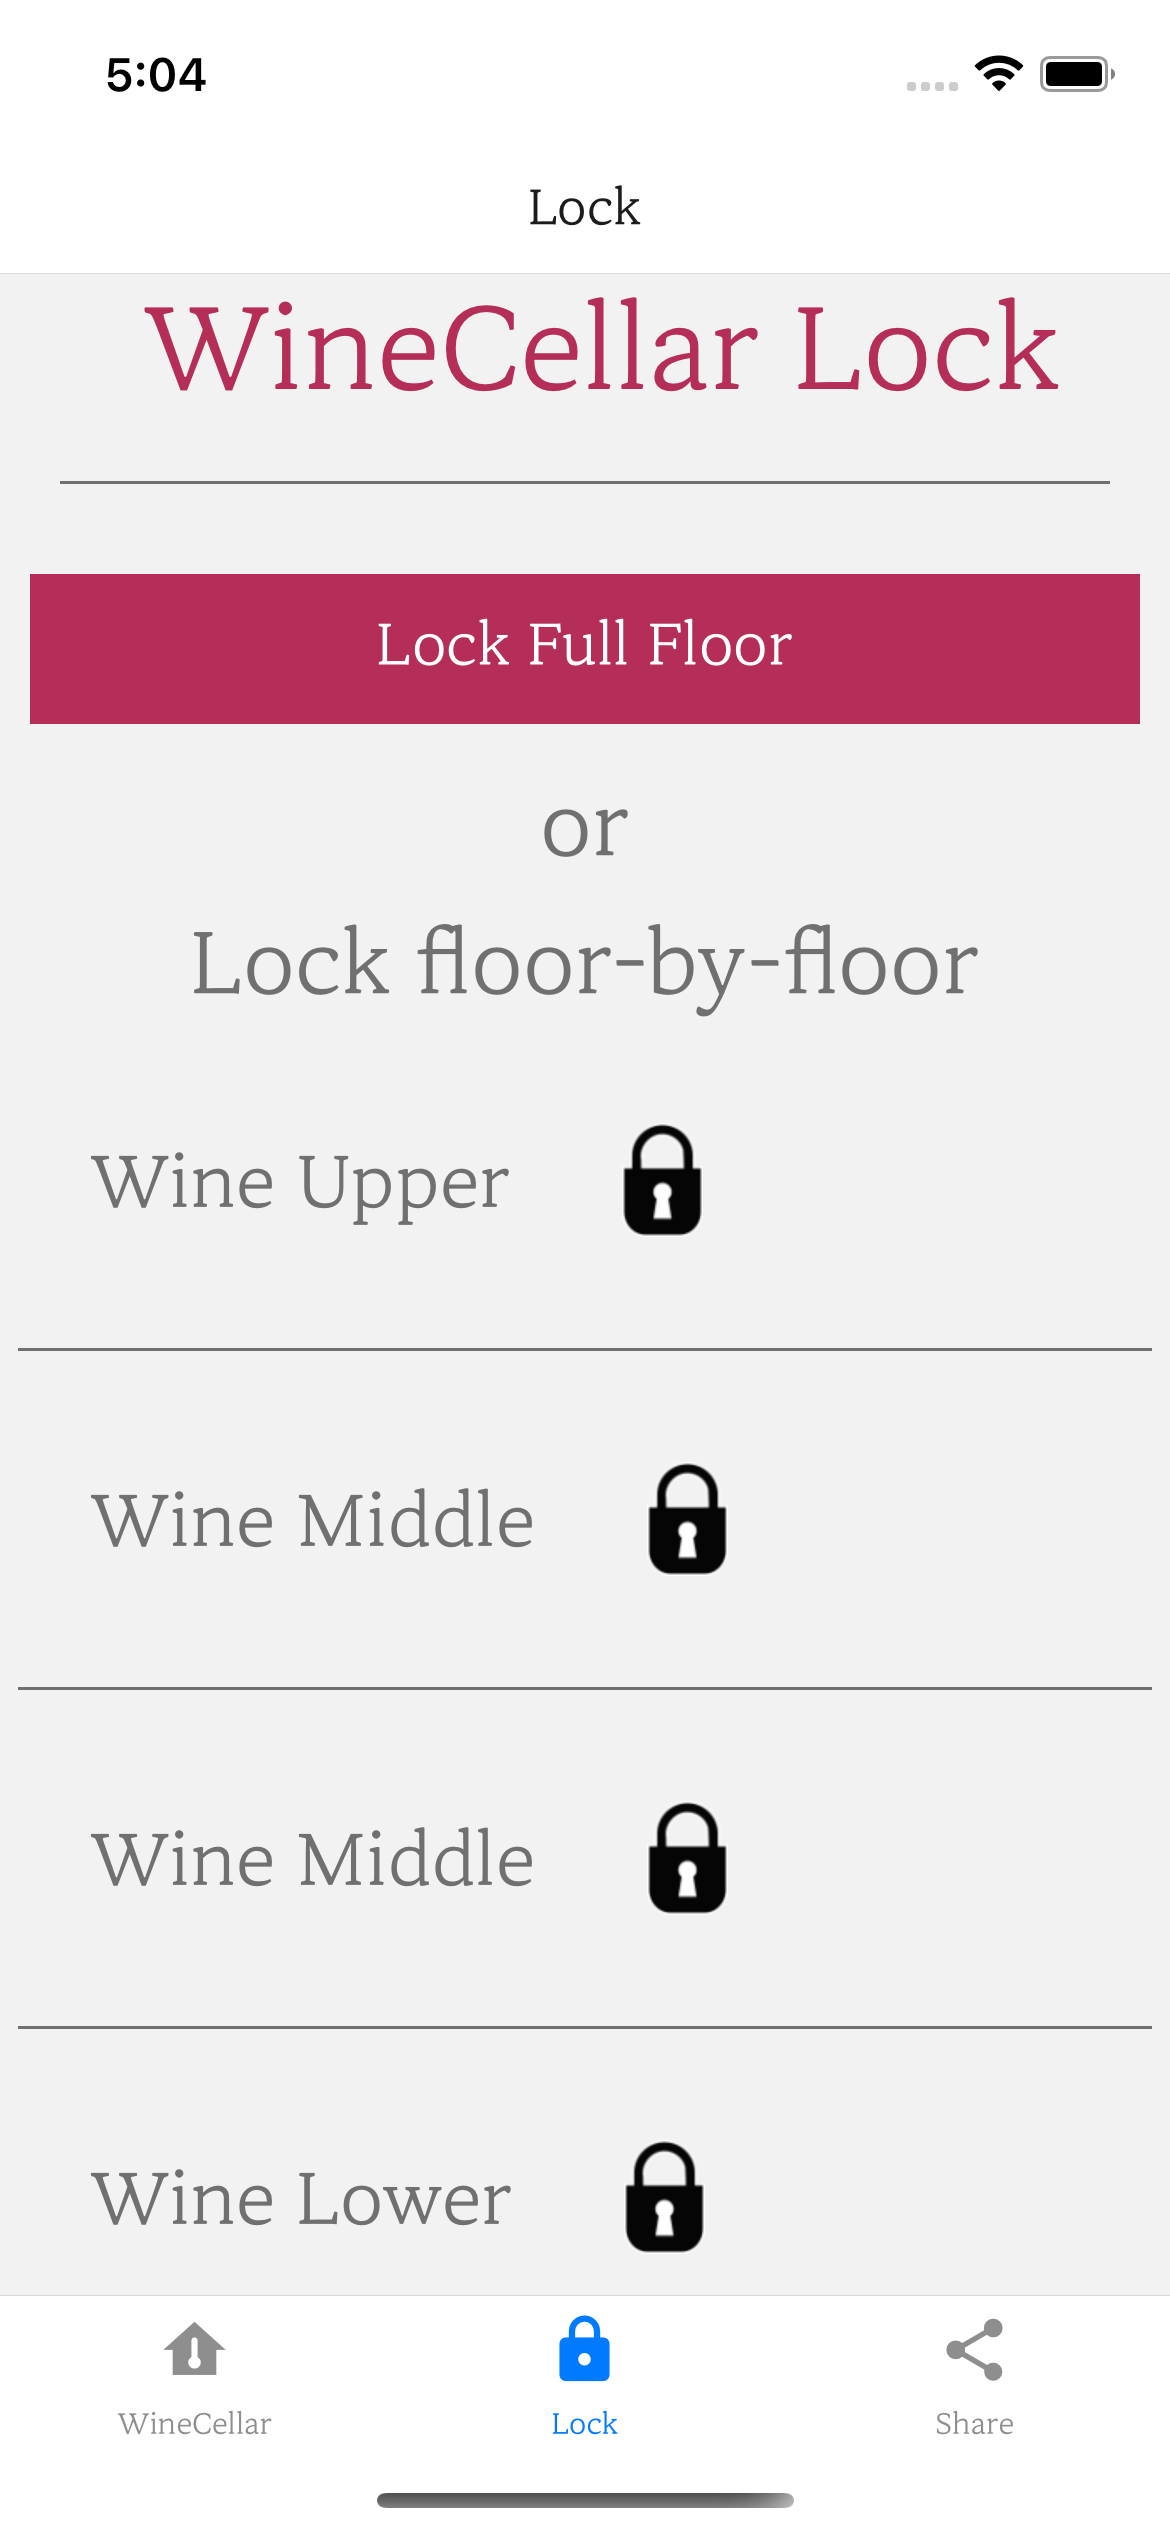
\includegraphics[width=5cm]{5. ViewingCellarTrytoLock.png}
                \caption{Password Setting}
            \end{figure}
            \begin{figure}[ht]
                \centering
                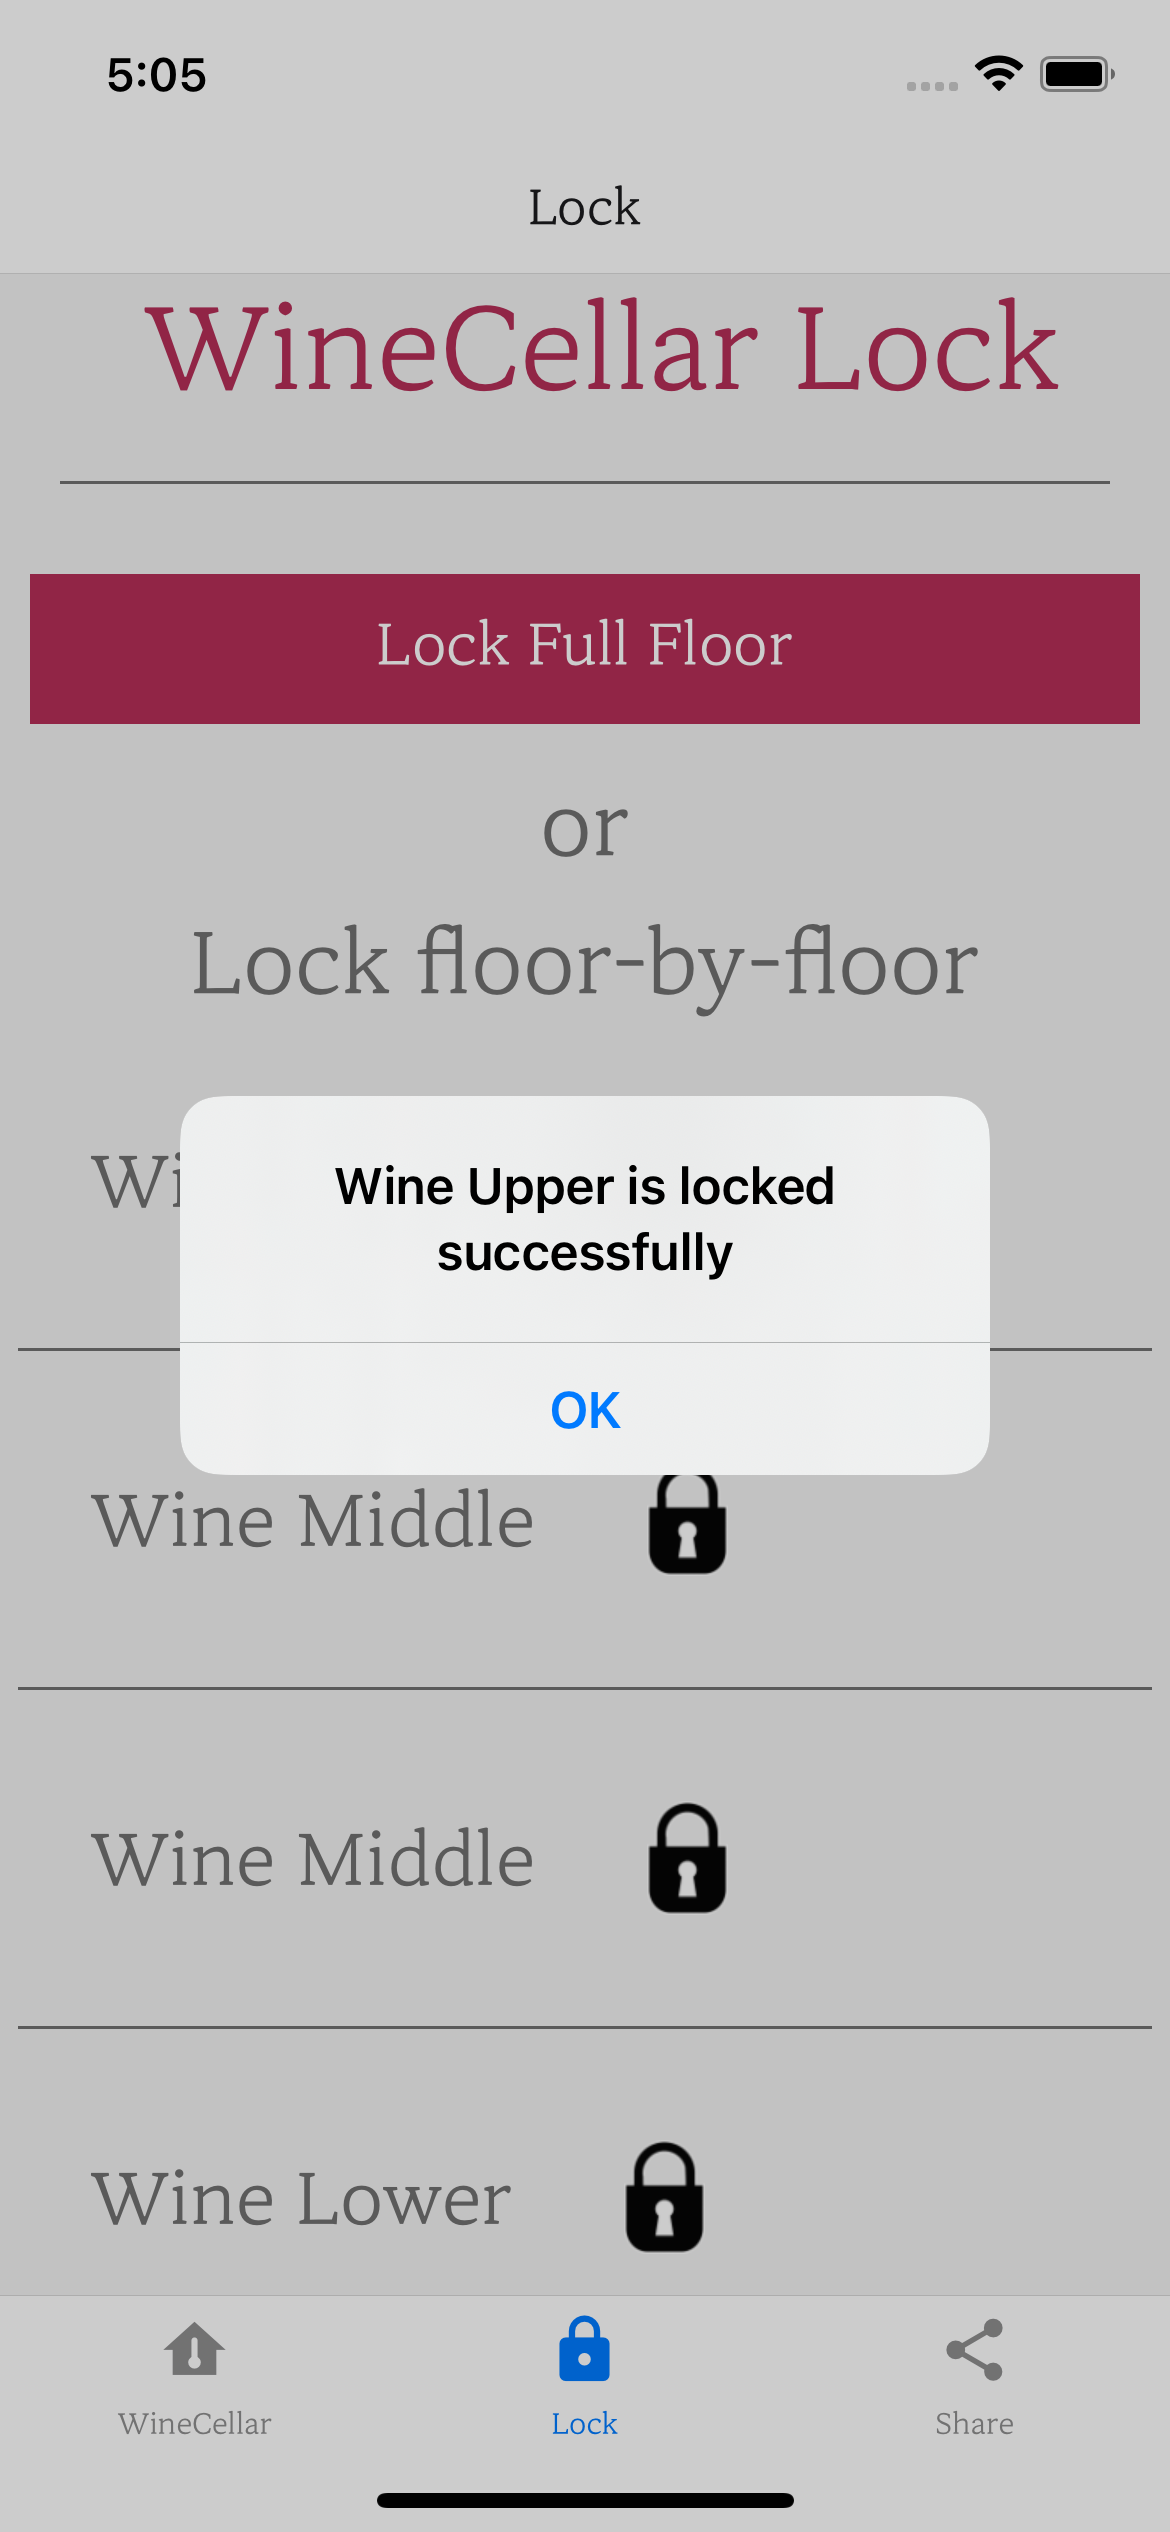
\includegraphics[width=5cm]{6.PartiallyLoced.png}
                \caption{Password Setting}
            \end{figure}
        \end{comment}
        Before entering Lock Page, user must set 6-digit password of the wine cellar. The password is encrypted and saved in the server's database. 
        \item Password: Saved\\
        %\centerline{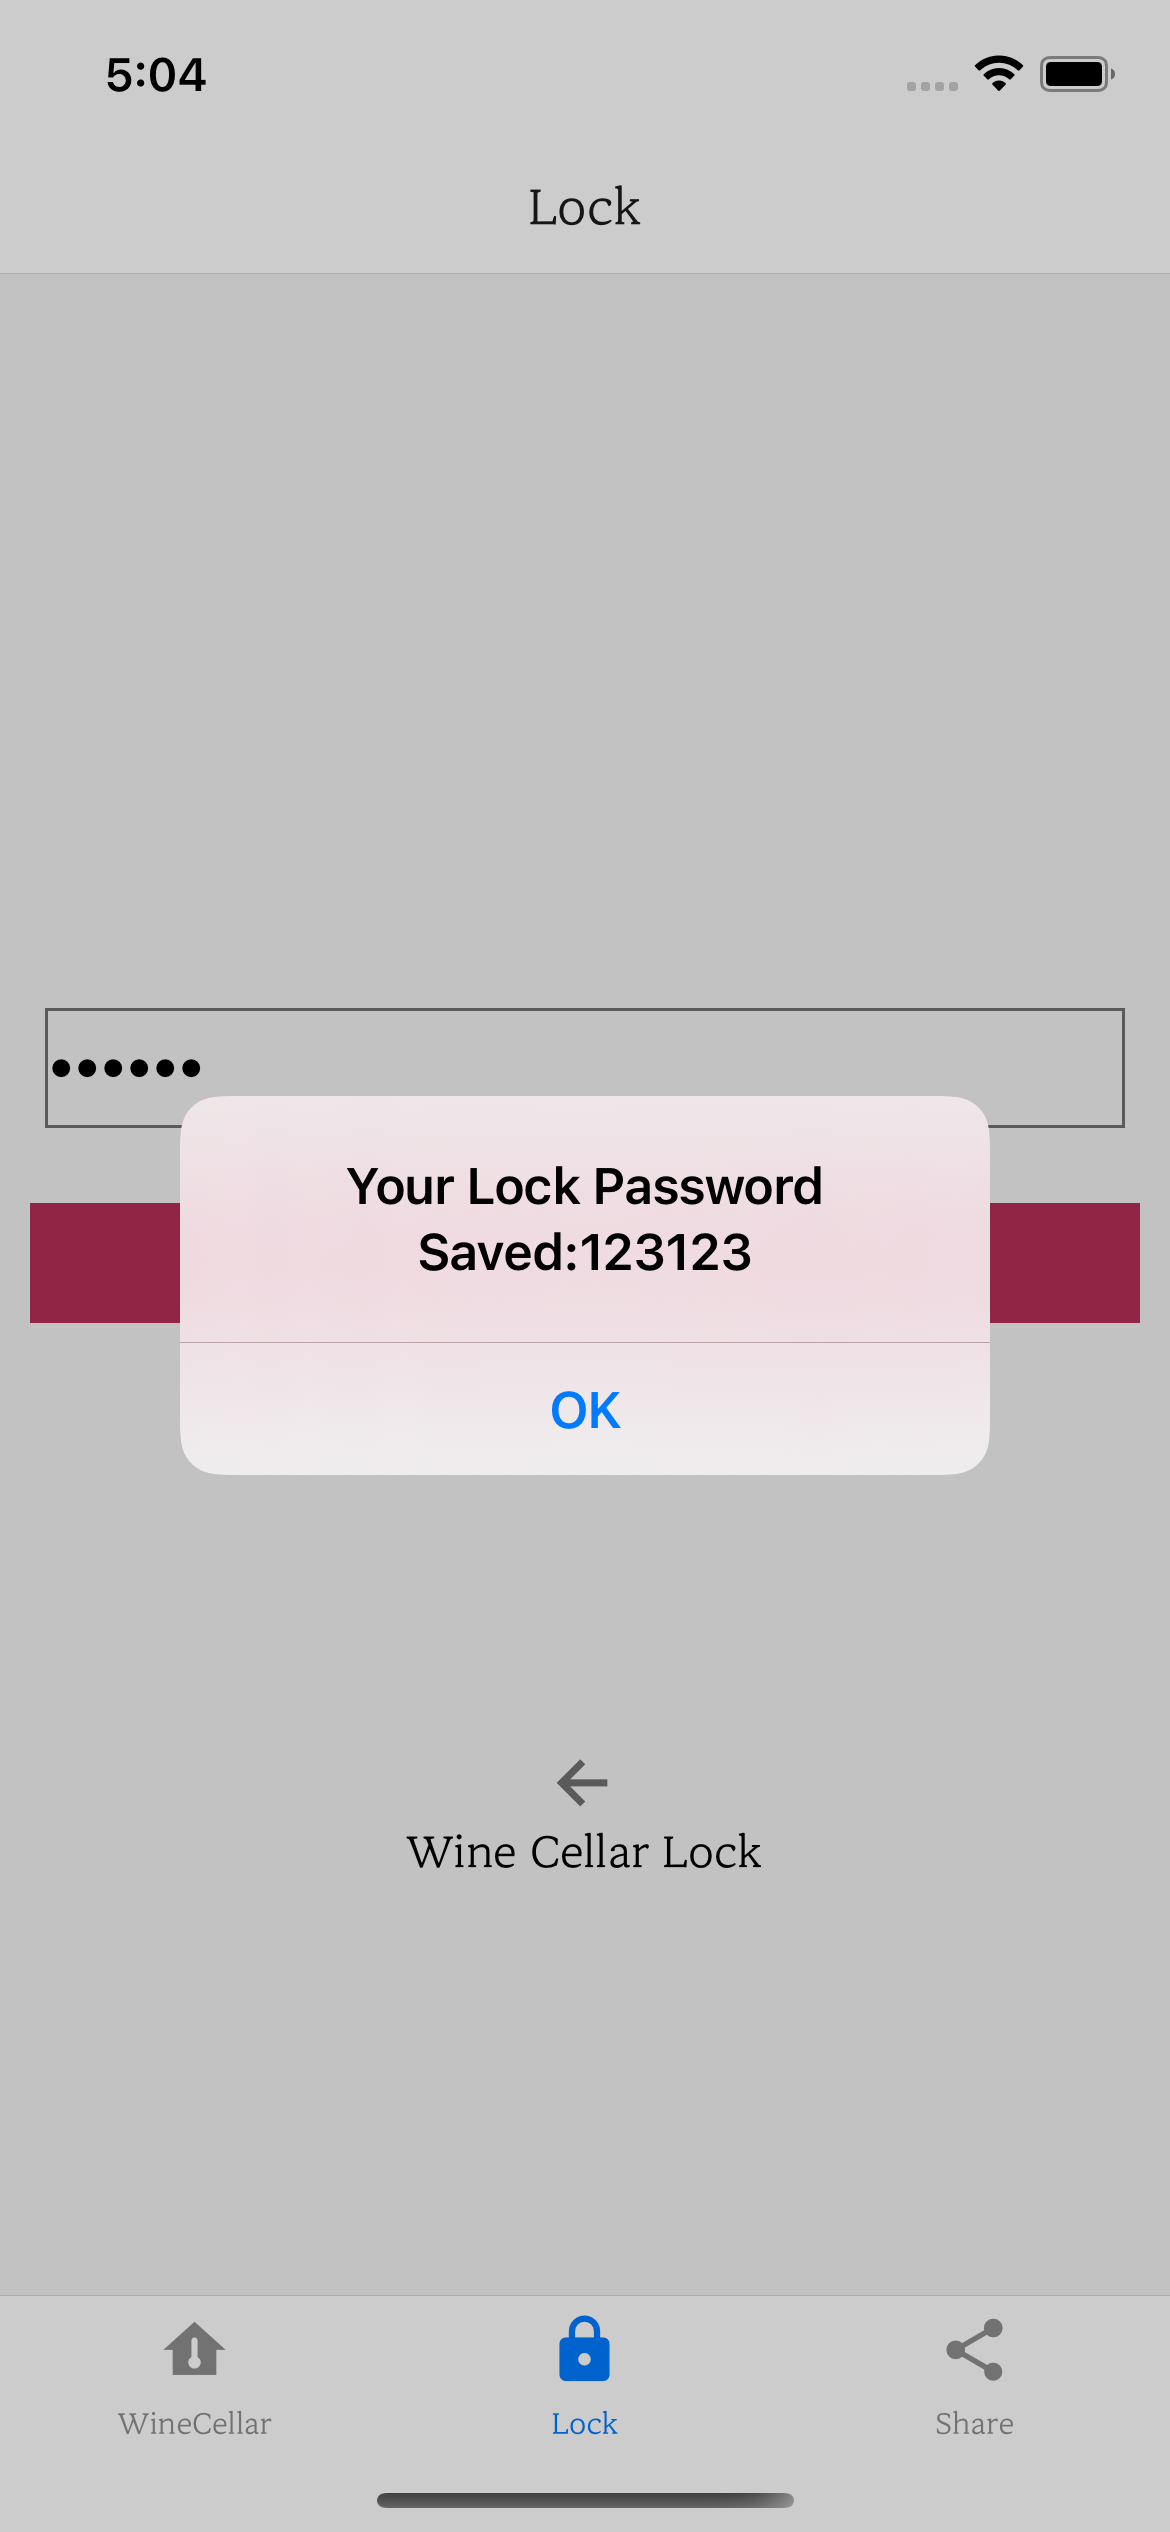
\includegraphics[width=5cm]{3. Winecellar AfterSetPasswd.png}}
        After pressing Save button, pop-up window appears with user's password. 
        \item Wine Cellar Main Page: Enter Password\\
        %\centerline{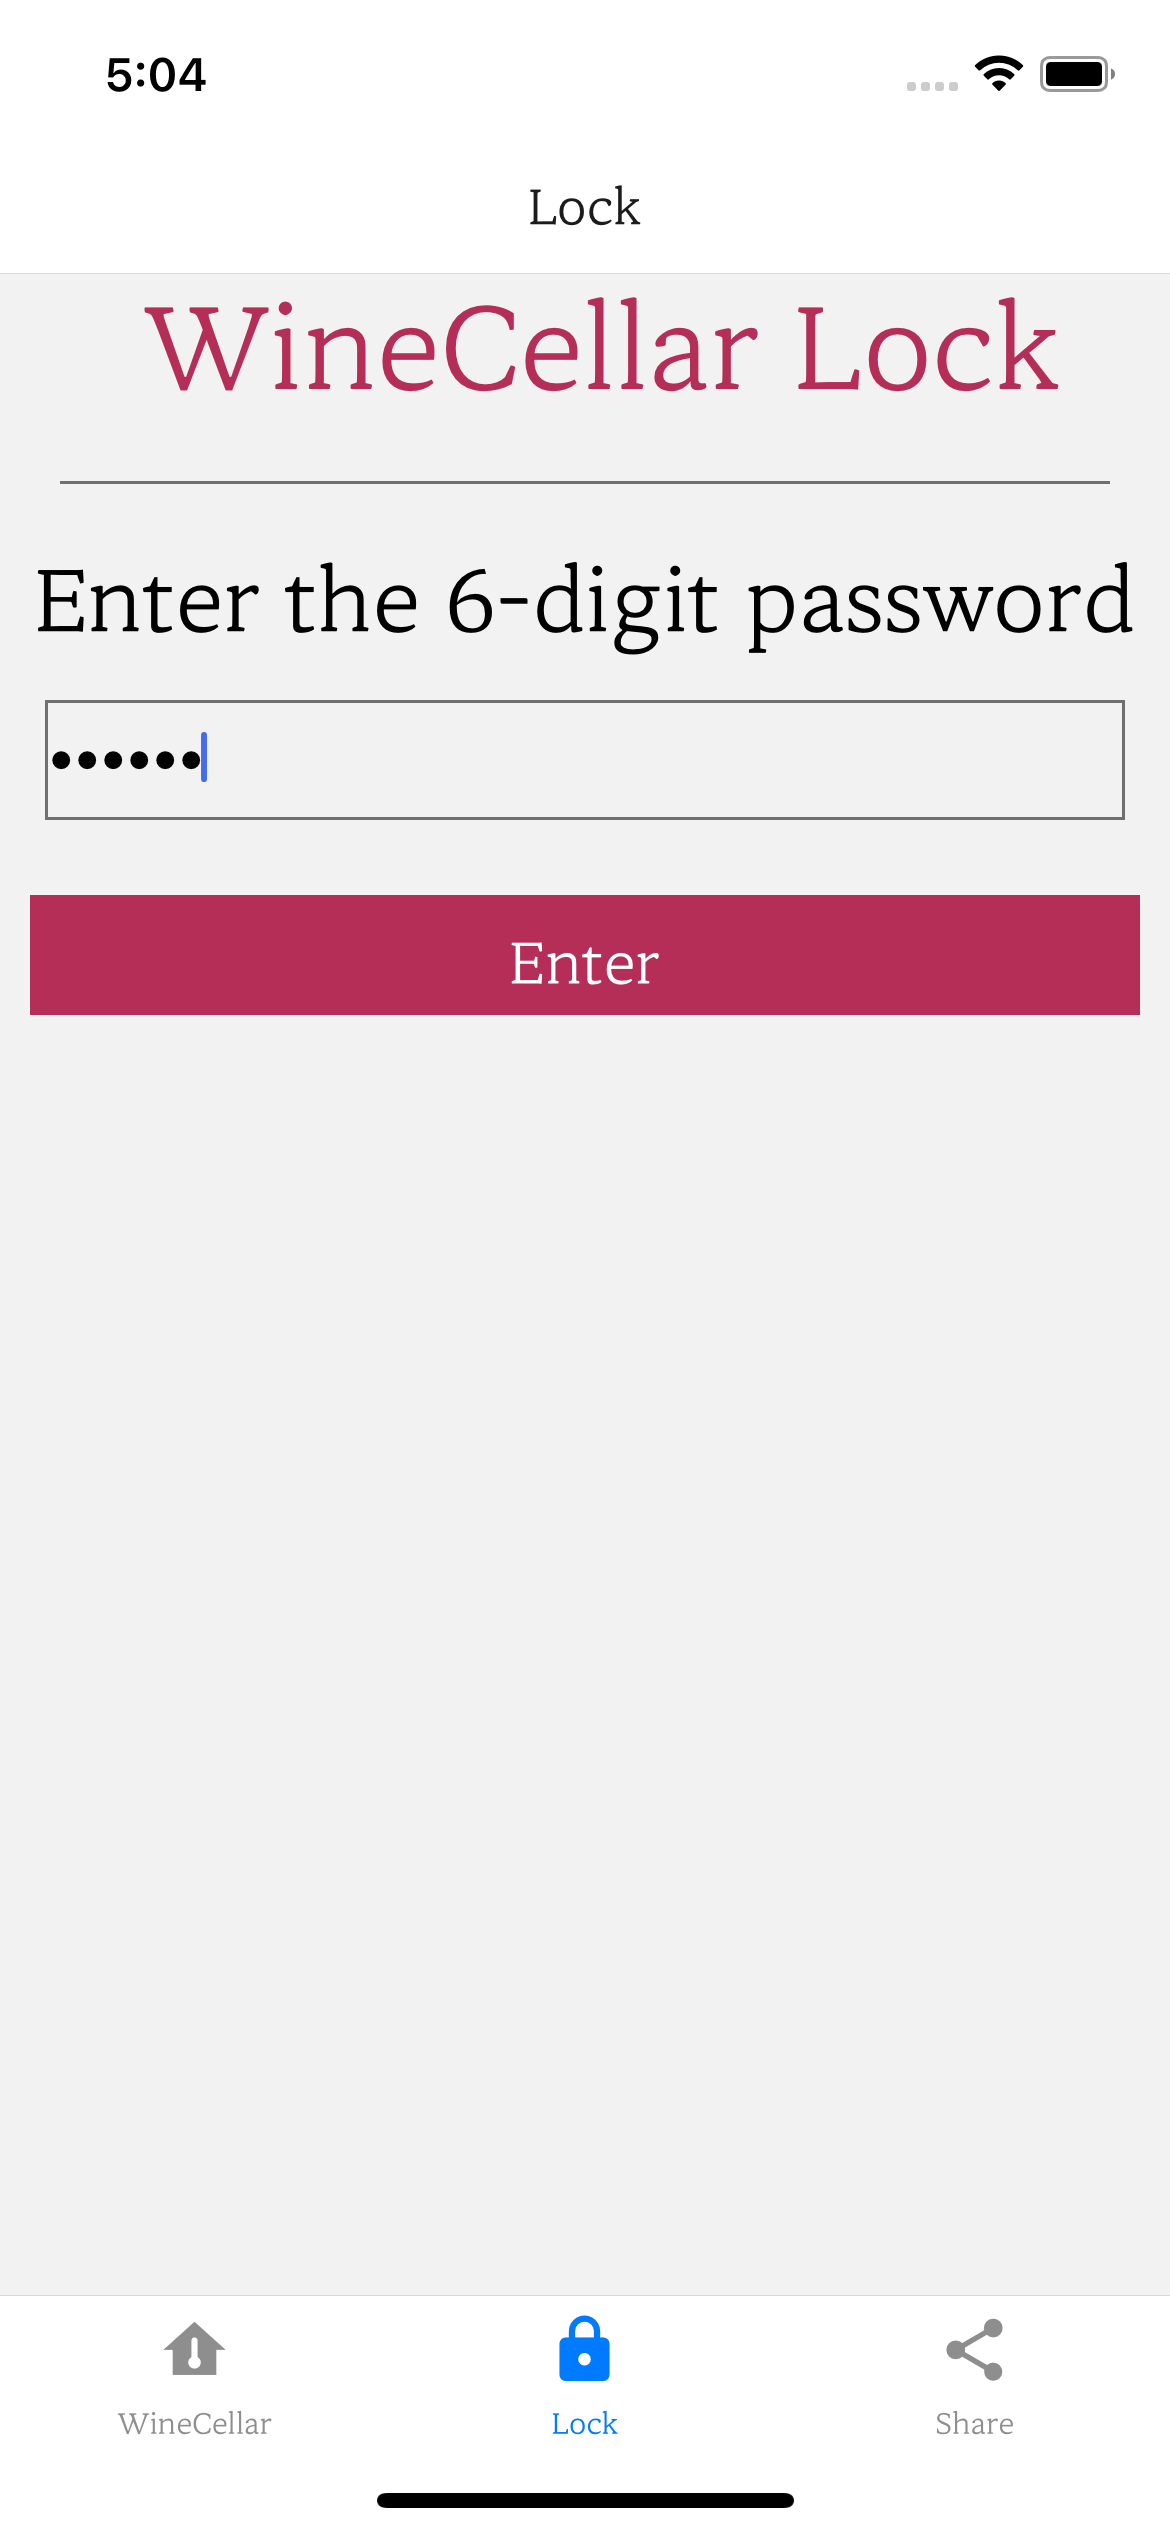
\includegraphics[width=5cm]{4. Passwd Confirmation.png}}
        After setting the password, user goes to the 'Wine Cellar Main Page : Enter Password'.
        %\centerline{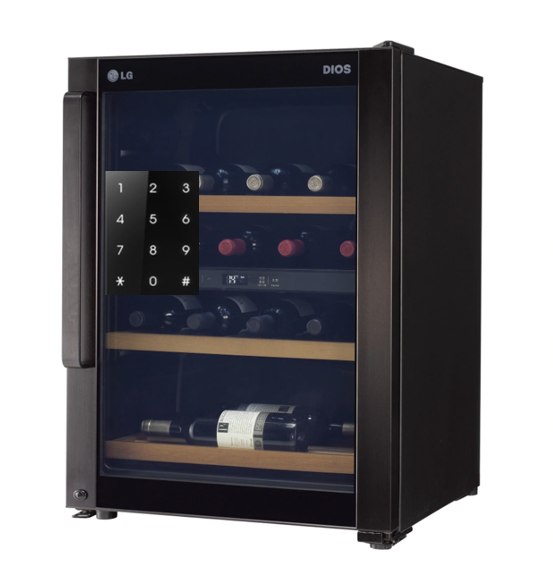
\includegraphics[width=5cm]{physicalwinecellar.png}}
        The same password applies in the physical winecellar which has transparent digital lock. 
        \item WineCellar Lock: Main Page\\
        %\centerline{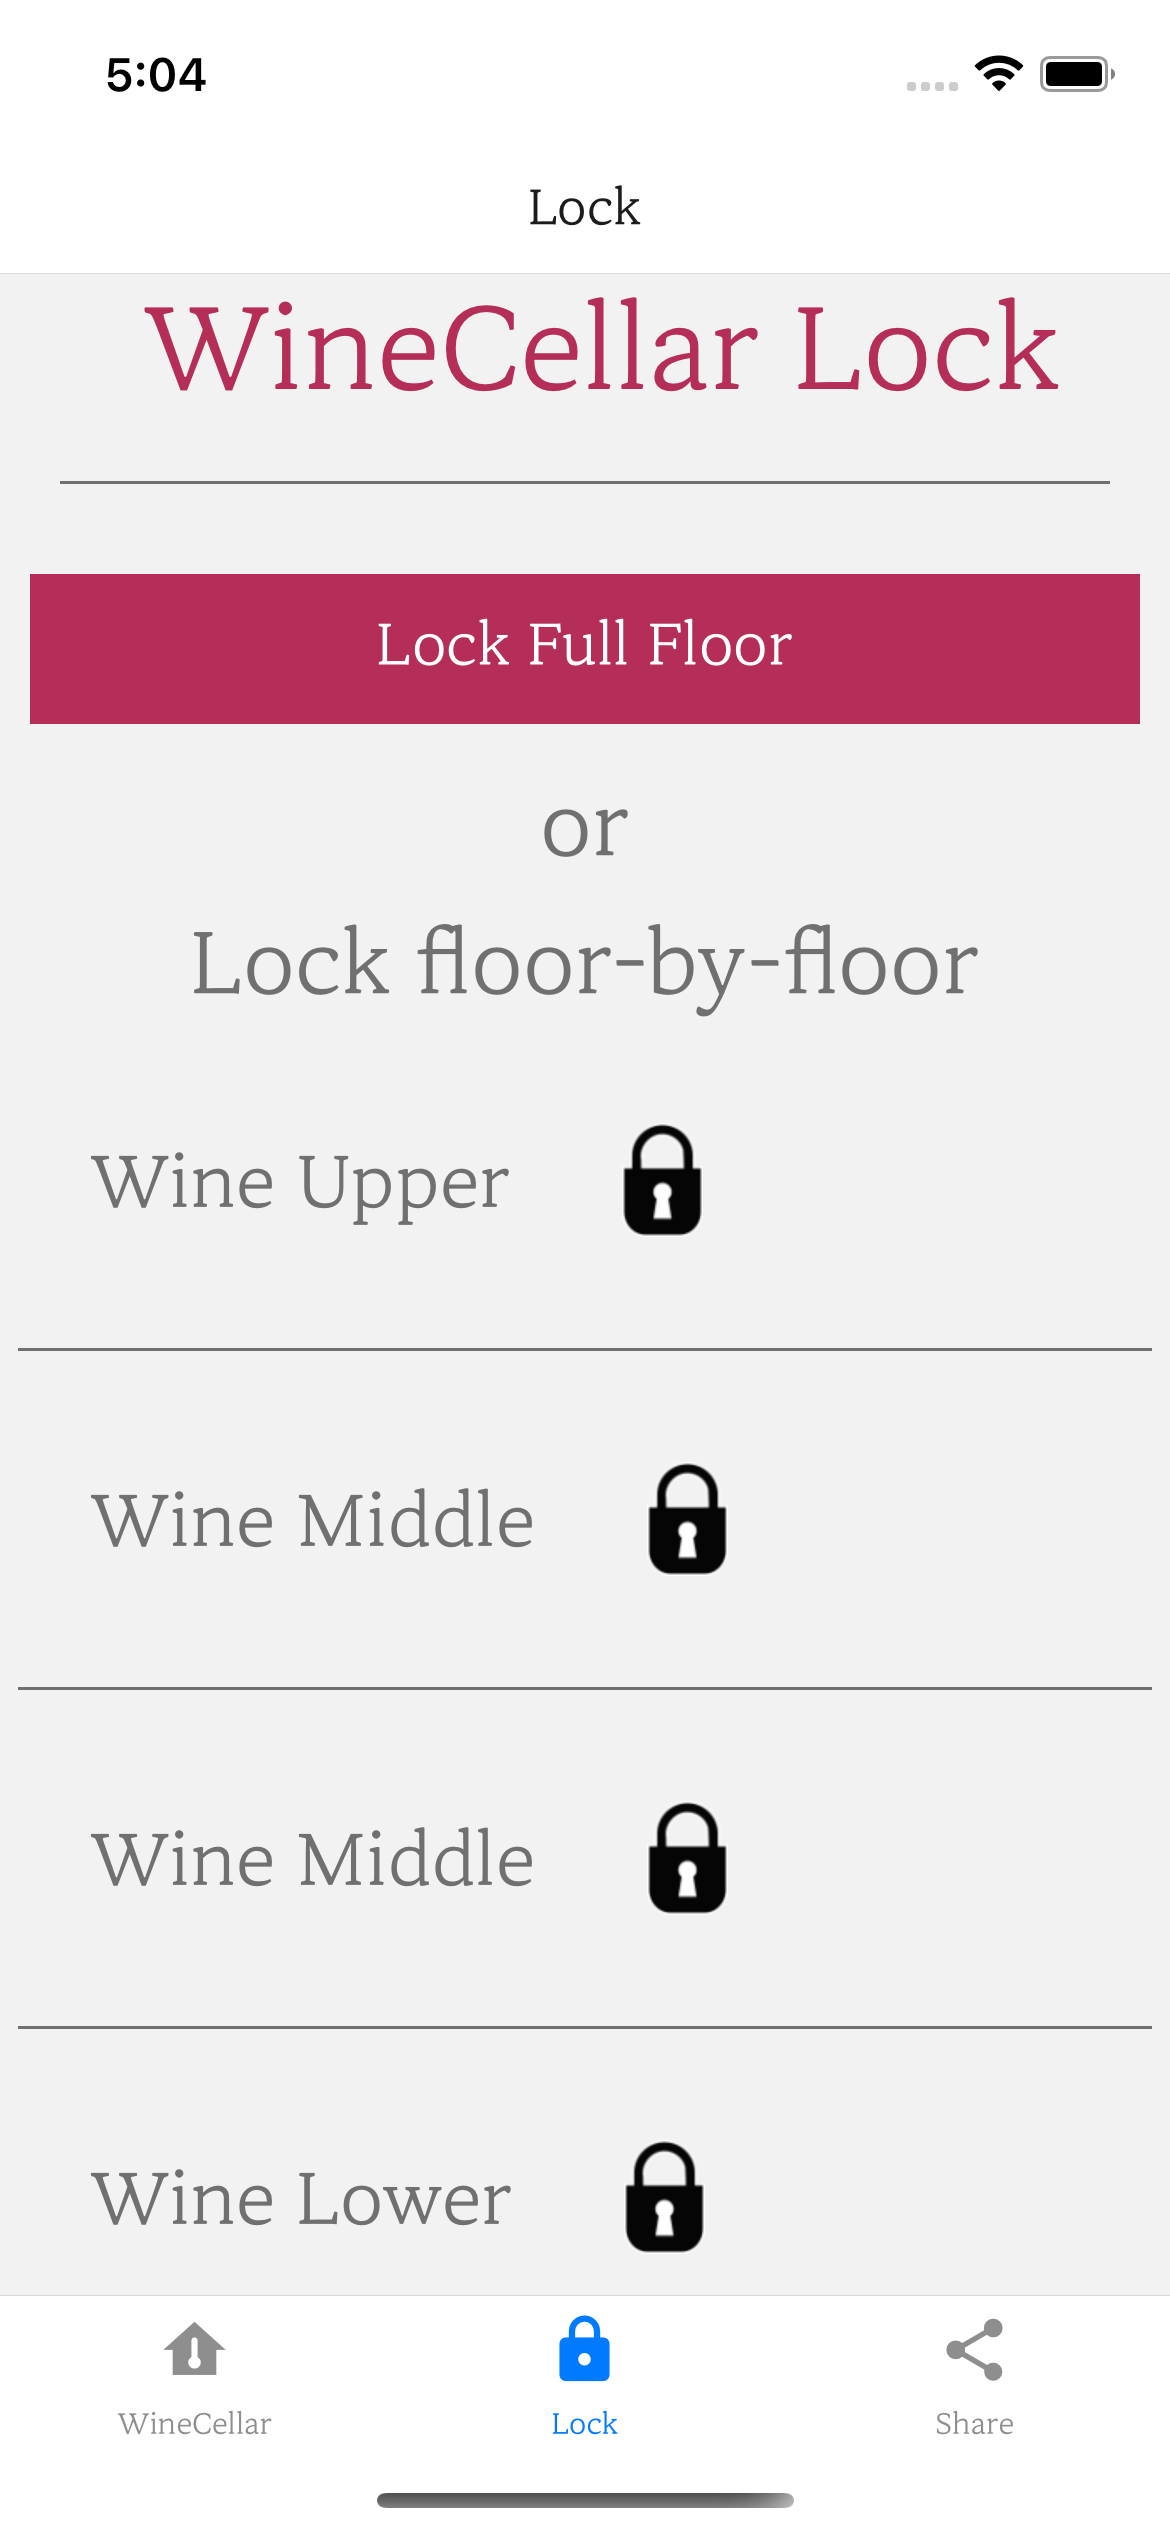
\includegraphics[width=5cm]{5. ViewingCellarTrytoLock.png}}
        First, user can lock the full floor of the wine cellar by pressing the red button. Second, they can lock the floor-by-floor by pressing each lock icon.  
        \item Successful Lock\\
        %\centerline{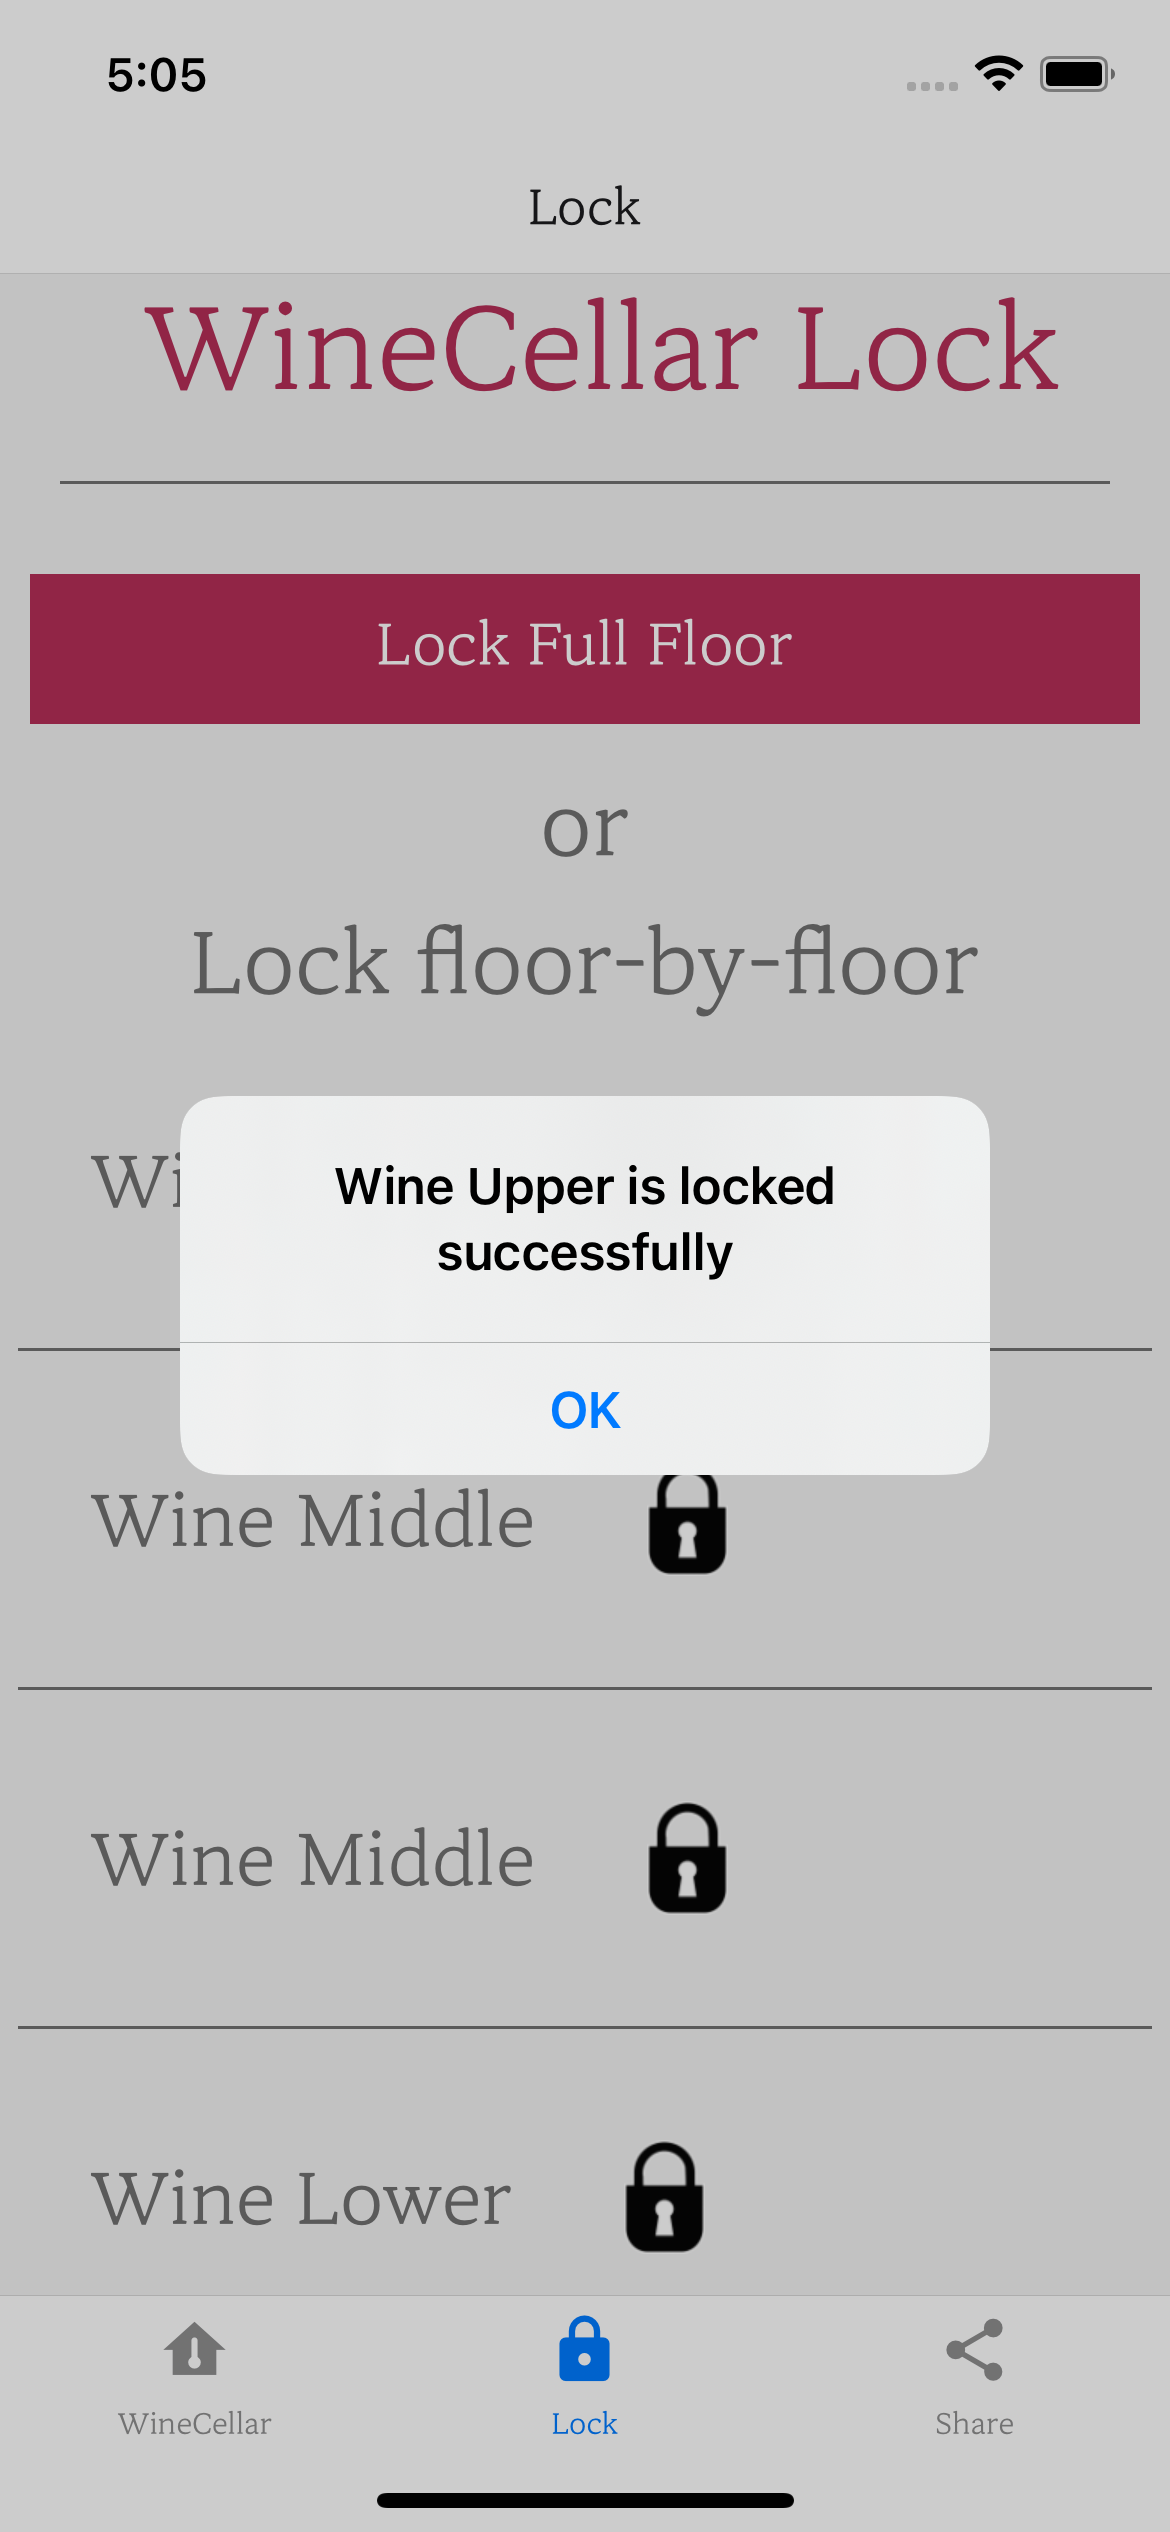
\includegraphics[width=5cm]{6.PartiallyLoced.png}}
        When lock is successful, pop-up window appears. 
    \end{enumerate}
    \item Share Page
    \begin{enumerate}
        \item Share My WineCellar
        \item Share My Wine History
        \item Make My Wine Topster
    \end{enumerate}
\end{enumerate}

\end{document}